%%%%%%%%%%%%%%%%%%%%%%%%%%%%%%%%%%%%%%%%%
% Masters/Doctoral Thesis 
% LaTeX Template
% Version 1.43 (17/5/14)
%
% This template has been downloaded from:
% http://www.LaTeXTemplates.com
%
% Original authors:
% Steven Gunn 
% http://users.ecs.soton.ac.uk/srg/softwaretools/document/templates/
% and
% Sunil Patel
% http://www.sunilpatel.co.uk/thesis-template/
%
% License:
% CC BY-NC-SA 3.0 (http://creativecommons.org/licenses/by-nc-sa/3.0/)
%
% Note:
% Make sure to edit document variables in the Thesis.cls file
%
%%%%%%%%%%%%%%%%%%%%%%%%%%%%%%%%%%%%%%%%%

%----------------------------------------------------------------------------------------
%	PACKAGES AND OTHER DOCUMENT CONFIGURATIONS
%----------------------------------------------------------------------------------------

\documentclass[11pt, twoside]{Thesis} % The default font size and one-sided printing (no margin offsets)

\graphicspath{{Pictures/}} % Specifies the directory where pictures are stored
%Para instalar dependencias en fedora
% sudo dnf install 'tex(titling.sty)'

\usepackage[spanish]{babel}
\usepackage{hyperref}
\usepackage{bmpsize}
\usepackage{multirow}
\usepackage{array}
\usepackage{tabularx}
\renewcommand\tabularxcolumn[1]{m{#1}}% for vertical centering text in X column

%\usepackage{xcolor}
\usepackage[table]{xcolor}
\usepackage{colortbl}


\usepackage{booktabs}% http://ctan.org/pkg/booktabs
\newcommand{\tabitem}{~~\llap{\textbullet}~~}

\usepackage{float}
\usepackage{url}
\usepackage[square, numbers, comma, sort&compress]{natbib} % Use the natbib reference package - read up on this to edit the reference style; if you want text (e.g. Smith et al., 2012) for the in-text references (instead of numbers), remove 'numbers'
\usepackage{bera}% optional: for a nice monospaced font
\usepackage{listings}
%\usepackage{svg} 
\usepackage{multicol}
\usepackage{float}

\newenvironment{Figure}
{\par\medskip\noindent\minipage{\linewidth}}
{\endminipage\par\medskip}
	
\newcommand{\steveCabecera}[1]{
	\fancyhead{}
	\fancyhead[LE,RO]{\footnotesize \thepage}
	\fancyhead[LO,RE]{\footnotesize #1}
}

\usepackage{caption}
\hypersetup{urlcolor=black, colorlinks=true} % Colors hyperlinks in blue - change to black if annoying
	\title{\ttitle} % Defines the thesis title - don't touch this

\begin{document}

\frontmatter % Use roman page numbering style (i, ii, iii, iv...) for the pre-content pages

\setstretch{1} % Line spacing of 1.3

% Define the page headers using the FancyHdr package and set up for one-sided printing
\fancyhead{} % Clears all page headers and footers
\rhead{\thepage} % Sets the right side header to show the page number
\lhead{} % Clears the left side page header

\pagestyle{fancy} % Finally, use the "fancy" page style to implement the FancyHdr headers

\newcommand{\HRule}{\rule{\linewidth}{0.5mm}} % New command to make the lines in the title page

% PDF meta-data
\hypersetup{pdftitle={\ttitle}}
\hypersetup{pdfsubject=\subjectname}
\hypersetup{pdfauthor=\authornames}
\hypersetup{pdfkeywords=\keywordnames}

%----------------------------------------------------------------------------------------
%	TITLE PAGE
%----------------------------------------------------------------------------------------

\begin{titlepage}
\begin{center}
\textsc{\LARGE \univname}\\[1.5cm] % University name


\begin{figure}[htbp]
	\centering
		\includegraphics[width=0.4\textwidth]{Figures/logo.png}
		\rule{35em}{0.5pt}
\end{figure}


\textsc{\Large Proyecto Integrador de Ingeniería en Computación}\\[0.5cm] % Thesis type

\HRule \\[0.4cm] % Horizontal line
{\huge \bfseries \ttitle}\\[0.4cm] % Thesis title
\HRule \\[1cm] % Horizontal line
 
\begin{minipage}[t]{0.4\textwidth}
\begin{flushleft} \large
\emph{Autor:}\\
{\authornames}\\ % Author name - remove the \href bracket to remove the link
\emph{Matrícula:}35.104.714
\end{flushleft}
\end{minipage}
\begin{minipage}[t]{0.4\textwidth}
\begin{flushright} \large
\emph{Director Docente:} 
\\{Mg.Ing. Miguel \textsc{Solinas} }\\ % Supervisor name - remove the \href bracket to remove the link  
\end{flushright}
\end{minipage}

\facname\\\groupname\\~\\ % Research group name and department name
 
{\large \today}\\ % Date
%\includegraphics{Logo} % University/department logo - uncomment to place it
\vfill
\end{center}
\end{titlepage}

\clearpage % Start a new page

%----------------------------------------------------------------------------------------
%	ABSTRACT PAGE
%----------------------------------------------------------------------------------------
\newpage

%----------------------------------------------------------------------------------------
%	LIST OF CONTENTS/FIGURES/TABLES PAGES
%----------------------------------------------------------------------------------------

\pagestyle{fancy} % The page style headers have been "empty" all this time, now use the "fancy" headers as defined before to bring them back

\lhead{\emph{Contenido}} % Set the left side page header to "Contents"
\tableofcontents % Write out the Table of Contents

\lhead{\emph{Lista de Figuras}} % Set the left side page header to "List of Figures"
\listoffigures % Write out the List of Figures
\listoftables
%\lhead{\emph{Lista de Tablas}} % Set the left side page header to "List of Tables"
%\listoftables % Write out the List of Tables

%----------------------------------------------------------------------------------------
%	ABBREVIATIONS
%----------------------------------------------------------------------------------------

\clearpage % Start a new page

\setstretch{1.2} % Set the line spacing to 1.5, this makes the following tables easier to read

%\lhead{\emph{Abreviaturas}} % Set the left side page header to "Abbreviations"
%\listofsymbols{ll} % Include a list of Abbreviations (a table of two columns)
%{
%\textbf{IEEE} & \textbf{I}nstitute of \textbf{E}lectrical and \textbf{E}lectronics \textbf{E}ngineers\\
%\textbf{SO} & \textbf{S}istema \textbf{O}perativo  \\
%\textbf{KDS} & \textbf{K}inetis \textbf{D}esign \textbf{S}tudio \\
%%\textbf{Acronym} & \textbf{W}hat (it) \textbf{S}tands \textbf{F}or \\
%}


%----------------------------------------------------------------------------------------
%	THESIS CONTENT - CHAPTERS
%----------------------------------------------------------------------------------------

\mainmatter % Begin numeric (1,2,3...) page numbering

\pagestyle{fancy} % Return the page headers back to the "fancy" style

% Include the chapters of the thesis as separate files from the Chapters folder
% Uncomment the lines as you write the chapters

% Chapter Template

\chapter{Introducción} % Main chapter title

\label{Chapter1} % Change X to a consecutive number; for referencing this chapter elsewhere, use \ref{ChapterX}

\steveCabecera{Capítulo 1. \emph{Introducción}} % Change X to a consecutive number; this is for the header on each page - perhaps a shortened title

El presente informe documenta el proyecto integrador del alumno que suscribe para la carrera Ingeniería en Computación de la FCEFyN de la UNC. Se trata de una aplicación para teléfonos android codificada enteramente en Java aplicando el paradigma de programación reactiva sobre Clean Architecture. Este proyecto se desarrolló como parte de un producto IoT destinado al control de accesos físicos a inmuebles.

Este informe contempla la etapa análisis de requerimientos y de diseño del producto en su conjunto ya que fue necesaria la coordinación de los integrantes del equipo para iniciar el desarrollo. Una vez establecidos los protocolos empleados y las interfaces de comunicación entre los componentes, el procesos de desarrollo del software de la aplicación se realizó de manera independiente.

Desde el punto de vista académico la mayor contribución de este proyecto se centra en la ingeniería de software involucrada en adaptar la solución a los lineamientos de un patrón de arquitectura estricto como lo es Clean Architecture. Al mismo tiempo, con el ánimo de ofrecer una implementación moderna y siguiendo la recomendación de exponentes de la industria, se asumió el reto de aplicar el paradigma de programación reactivo de manera transversal en el proyecto.

Al finalizar el proyecto se obtuvo la primera versión del producto que pudo ser evaluada con usuarios reales.
%el diseño del sistema completo, en conjunto con el responsable del sistema embebido (módulo electrónico). 

\section{Motivación}
%La motivación del producto en su conjunto nace de la necesidad de ofrecer un upgrade a los sistemas tradicionales de control de accesos ofrecidos en el mercado. Tras demostrarse 
Como se mencionó anteriormente el presente proyecto forma parte de un producto IoT destinado al control de accesos físicos a inmuebles.
A su vez este producto forma parte del plan de negocios de un emprendimiento que fue admitido en la incubadora de empresas de la UNC.

La idea del proyecto nació luego de que se reportaran en los medios una sucesión de entraderas a domicilios en varios puntos de la ciudad de Córdoba. La mayoría de estos actos criminales se fueron perpetrados con el uso de inhibidores de señal que interferían con los controles remotos RF de portones automatizados. Otro caso llamativo se llevaba a cabo mediante la clonación de llaves RFID en las cerraduras magnéticas de las puertas de ingreso en edificios de departamentos. Se detectó, entonces, la necesidad de contar con una alternativa moderna a los sistemas de control tradicionales ofrecidos actualmente en el mercado.

\section{Objetivos}
Los objetivos del proyecto se desprenden de la propuesta de valor del producto. El general está asociado a la visión del emprendimiento.
Y los particulares relacionados a el proceso de desarrollo del producto en sí.
\subsection{General}
Diseñar, implementar y validar una aplicación para teléfonos android que permita la configuración, el control y el monitoreo de sistemas de acceso físicos a inmuebles. 

\subsection{Objetivos Particulares}

\begin{itemize}
	\item Relevar documentación sobre cerramientos eléctricos.
	\item Conseguir una descripción sistémica de los mismos y encontrar una propuesta de adaptación para la solución propuesta.
	\item Definir los casos de uso y requerimientos para los desarrollos de software.
	\item Diseñar la solución en conjunto. Definir protocolos de comunicación y establecer al interfaz de comunicación entre los componentes.
	\item Investigar y documentar el patrón de arquitectura de software elegido.
	\item Investigar sobre el paradigma de programación reactiva y su utilización empleando Java.
	\item Implementar el diseño especificado.
	\item Validar dicha implementación con pruebas automáticas.
\end{itemize}

\section{Metodología de Trabajo}
%Se utilizará un panel tipo kanban para el registro del progreso de tareas de desarrollo. Las tareas serán marcadas con  
Todo la codificación se realizará utilizando el sistema de gestión de versiones git en un repositorio privado alojado remotamente en bitbucket. Al ser un proyecto con un único programador la resolución de tareas se realizará en ramas auxiliares con origen en \textbf{develop}. Una vez terminado el trabajo en una rama auxiliar se procederá a hacer un rebase con develop y a la correspondiente re-escritura de commits para facilitar la lectura a futuro. La rama master contendrá solo las cambios cuyos ejecutables fueron distribuidos a través de la play store de android.


% Chapter Template

\chapter{Marco Teórico} % Main chapter title

\label{Chapter2} % Change X to a consecutive number; for referencing this chapter elsewhere, use \ref{ChapterX}

%\fancyhead{}
%\fancyhead[LE,RO]{\thepage}
%\fancyhead[LO,RE]{Capítulo 2. \emph{Marco Teórico}} % Change X to a consecutive number;
\steveCabecera{Capítulo 2. \emph{Marco Teórico}}
%\rhead{Capítulo 2. \emph{Marco Teórico}} % Change X to a consecutive number; this is for the header on each page - perhaps a shortened title

\section{Cerramientos Eléctricos}
Cuando hablamos de cerramientos eléctricos se hacer referencia a todos los dispositivos
de funcionamiento electromecánico destinados a ofrecer la función de cerradura para aperturas de instalaciones domiciliarias, comerciales e industriales.
Se listan a continuación ejemplos de estos dispositivos.
\begin{itemize}
	\item Cerraduras por electro-imán.
	\item Cerraduras de perno.
	\item Portones automatizados.
	\item Barreras automáticas.
	\item Pasadores eléctricos.
	\item Traba-pestillo eléctrico.
	\item Pestillo eléctrico para cajones o guarda equipajes.
	\item Puertas de Ascensor con control de acceso.
\end{itemize}


\subsection{Principio de Funcionamiento}
Aunque todos los cerramientos eléctricos comparten la misma funcionalidad existe una variedad acotada de principios de funcionamiento, diseño industrial o factor de forma entre los cuales podemos mencionar:
\begin{itemize}
	\item Solenoide y Perno
	\item Solenoide y Clavija
	\item Electro-imán
	\item Motor Eléctrico
\end{itemize}

\subsubsection{Solenoide y Perno}
Un solenoide es enrollado alrededor de un eje cilíndrico dieléctrico hueco que a su vez envuelve un perno también cilíndrico pero metálico. Este solenoide está conectado en un circuito de corriente continua. Cuando se alimenta dicho circuito el campo magnético inducido en el núcleo del solenoide genera corrientes de Foucault sobre el perno que es desplazado por la fuerza del campo magnético, generando así la acción de traba o bloqueo sobre el herraje de la abertura. 
Este tipo de principio de funcionamiento es el que emplean dispositivos tales como los pestillos eléctricos y las cerraduras de perno que se muestran en la figura ~\ref{fig:sol+perno}.

\begin{figure}[htbp]
	\centering
	\includegraphics[width=0.5\textwidth]{Pictures/sol+perno.png}
	\rule{35em}{1pt}
	\caption[Cerramientos de perno]{Se muestran ejemplos de cerramientos eléctricos que funcionan con solenoide y perno. }
	\label{fig:sol+perno}
\end{figure}

\subsubsection{Solenoide y Clavija}
De una forma similar a la descripta para el caso del perno, un solenoide se utiliza para formar un pequeño electroimán en el interior del dispositivo. La fuerza inducida deforma de manera elástica una clavija o chapa metálica delgada en forma de ele. Esta deformación libera el mecanismo que bloquea el movimiento del pestillo. Este es el caso del traba-pestillo eléctrico o del pasador eléctrico cuyos ejemplos se muestran en la figura ~\ref{fig:sol+clav}.

\begin{figure}[htbp]
	\centering
	\includegraphics[width=0.35\textwidth]{Pictures/sol+clav.png}
	\rule{35em}{1pt}
	\caption[Cerramientos de perno]{Se muestran ejemplos de cerramientos eléctricos que funcionan con solenoide y clavija. }
	\label{fig:sol+clav}
\end{figure}

\subsubsection{Electroimán}
En esta forma de funcionamiento se construye un electro-imán de dimensiones considerables capaz de ejercer una fuerza de atracción magnética cercana a los 300 kgF sobre una chapa metálica que también se incluye como parte del cerramiento. Por lo general incluyen en su circuito una etapa de compensación de factor de potencia para remanencia cero.
Este es el caso de la cerradura por electro-imán que se muestra en la figura ~\ref{fig:cerr-mag}.

\begin{figure}[htbp]
	\centering
	\includegraphics[width=0.4\textwidth]{Pictures/magnet.png}
	\rule{35em}{1pt}
	\caption[Cerradura Electroimán]{Se muestran un ejemplo de cerradura eléctrica que funcionan por electro-imán. }
	\label{fig:cerr-mag}
\end{figure}

\subsubsection{Motor Eléctrico}
Para el caso de grandes portones de garaje o acceso vehicular se utilizan motores de corriente alterna o brushless de corriente continua con su respectivos controladores. Estos motores interactúan mecánicamente con otras interfaces mecánicas instaladas en las aperturas para posibilitar la tarea de apertura o cierre. Adicionalmente es necesario la incorporación de sensores que indiquen el estado del sistema y aseguran su correcto funcionamiento.
Todos los tipos de automatización de portones así como los sistemas de apertura con cortinas metálicas comparten el mismo principio de funcionamiento y utilizan motores similares al que se muestra en la figura ~\ref{fig:motorport}.

\begin{figure}[htbp]
	\centering
	\includegraphics[width=0.4\textwidth]{Pictures/motor.png}
	\rule{35em}{1pt}
	\caption[Motor Portones Automatizados]{Motor empleado en sistemas de automatización de portones de garaje o accesos vehiculares. }
	\label{fig:motorport}
\end{figure}

\section{Controladores}
\label{section:controladores}
Todos los cerramientos eléctricos mencionados anteriormente no funcionan por si mismos sino que requieren de un dispositivo controlador.
Algunos ejemplos se muestran en la figura ~\ref{fig:controladoresacceso}.\\
\begin{figure}[htbp]
	\centering
	\includegraphics[width=0.8\textwidth]{Pictures/controladoresacceso.png}
	\rule{35em}{1pt}
	\caption[Controladores de Acceso]{Algunos ejemplos de controladores de cerramientos eléctricos.}
	\label{fig:controladoresacceso}
\end{figure}
Estos controladores son circuitos electrónicos que se encargan de generar las señales de activación y/o control de los cerramientos eléctricos. El usuario podrá actuar sobre el cerramiento eléctrico a través de diversos modos de accionamiento, se mencionan los más habituales:
\begin{itemize}
	\item Portero telefónico
	\item Contraseña por teclado
	\item Lector biométrico
	\item Llave electrónica
	\item Botón externo
\end{itemize}

Para dar soporte a una o múltiples formas de accionamiento el controlador ofrece una interfaz de configuración y los componentes necesarios para su operación.
En el caso de los cerramientos a motor es necesario incluir sensores de apertura y funcionamiento.

\subsection{Sensores}
Por lo general solo son empleados por los controladores para cerramientos a motor. Existen vario tipos de sensores para estos controladores se mencionan los más utilizados:
\begin{itemize}
	\item Sensores de Fin de Carrera
	\item Encoder Digital
\end{itemize}
. 
\subsubsection{Sensores de Fin de Carrera}
\label{section:fincarrera}
Se utiliza el plural para este caso de sensado porque se utilizan de a pares. Se trata de un par de sensores binarios que indican apertura o cierre total del cerramiento.
Suelen venir en dos presentaciones con modo de funcionamiento distinto.\\
\textbf{Por proximidad magnética:} En este caso cada uno de los sensores está compuesto por un imán permanente y un switch encapsulado como se muestra en la figura ~\ref{fig:fincarrera}(a). Este encapsulado contiene en su interior un filamento de material ferromagnético flexible que al aproximarse lo suficiente al imán se desplaza y cierra el circuito.\\
\textbf{Por choque mecánico:} Estos sensores son switches mecánicos muy sensibles que se instalan en los límites del marco de la abertura y al mínimo contacto con la parte móvil cierran sus circuitos. En la figura ~\ref{fig:fincarrera}(b) se muestran ejemplos de estos dispositivos.

\begin{figure}[htbp]
	\centering
	\includegraphics[width=0.6\textwidth]{Pictures/fincarrera.png}
	\rule{35em}{1pt}
	\caption[Sensores de fin de carrera]{Ejemplos de sensores de fin de carrera.(a) Sensores por proximidad magnética, (b) Sensores por choque mecánico. }
	\label{fig:fincarrera}
\end{figure}

\subsubsection{Encoder Rotativo}
Un encoder es un sensor de movimiento mecánico que genera señales digitales en respuesta al movimiento y puede proveer  información sobre la posición, la velocidad y la dirección del movimiento. En particular el econder rotativo responde al movimiento de rotación de un eje. Por lo general los controladores de cerramientos eléctricos a motor utilizan encoders rotativos incrementales que generan un tren de pulsos que se puede utilizar para determinar la posición y la velocidad del eje del motor. En la figura ~\ref{fig:encoder00} se observa la forma del tren de pulsos que genera el encoder.

\begin{figure}[htbp]
	\centering
	\includegraphics[width=0.8\textwidth]{Pictures/encoder00.png}
	\rule{35em}{1pt}
	\caption[Encoder Rotativo]{Ilustración simplificada de un encoder rotativo con salida de onda cuadrada TTL. }
	\label{fig:encoder00}
\end{figure}


\subsection{Monitoreo y Alerta}
La mayoría de los controladores poseen interfaces que permiten la conexión local de luminarias testigo, así como bocinas de alerta. Algunos modelos incluyen un puerto serie (RJ45, RJ14) capaz de comunicarse mediante comandos estándar con los tradicionales sistemas de alarma.

\subsubsection{Monitoreo Remoto}
Al momento de iniciar el presente proyecto integrador no existían controladoras de acceso con la funcionalidad de monitoreo remoto incorporada de fábrica.
La alternativa para tener información del cerramiento eléctrico y el estado de la abertura que opera consiste en instalar un sensor de apertura y conectarlo a una central de alarma. Estos sensores son baratos y su principio de funcionamiento coincide con el descripto para los sensores de fin de carrera y que se puede consultar en la sección ~\ref{section:fincarrera}.
Las centrales de alarma suelen estar conectadas por cableado telefónico a un servicio de monitoreo que lanza las notificaciones pertinentes según se hayan configurado.
Una basta mayoría de proveedoras de servicio de monitoreo de alarmas ahora ofrecen plataformas web o aplicaciones móviles que permiten el monitoreo de las centrales en tiempo real.

\subsection{Llaves Electrónicas y Control Remoto}
\label{section:llaves_electronicas}
Actualmente la mayoría de los controladores de acceso soportan algún tipo de llave electrónica.
Una llave electrónica es un dispositivo electrónico que le permite al usuario operar el cerramiento eléctrico. Existen diversos tipos de llaves electrónicas a continuación se mencionan las más utilizadas.
\begin{itemize}
	\item Llaves RFID
	\item Control Remoto RF
\end{itemize}

\subsubsection{Llaves RFID}
RFID (Radio-frequency identification) es un sistema de almacenamiento y recuperación de datos a distancias cortas por emisión de radiofrecuencia de baja potencia. 
Una etiqueta RFID consiste en un pequeño circuito receptor y transmisor de radio. Cuando es activada por un pulso de interrogación electromagnético emitido por un dispositivo lector RFID cercano, la etiqueta transmite datos digitales de vuelta al lector, generalmente un número identificador.
Estas etiquetas o circuitos RFID son tan diminutos que pueden incluirse en objetos de tamaño reducido como llaveros y tarjetas, algunos ejemplos se muestran en la figura ~\ref{fig:llavesrfid}.
El usuario del sistema de acceso aproximará esta llave al lector RFID incluido en el controlador y se producirá el intercambio del número identificatorio. En caso de que ese dato esté registrado en el controlador el usuario podrá controlar el cerramiento eléctrico.

\begin{figure}[htbp]
	\centering
	\includegraphics[width=0.8\textwidth]{Pictures/llavesrfid.png}
	\rule{35em}{1pt}
	\caption[Llaves RFID]{Llaveros y tarjetas con etiquetas RFID. }
	\label{fig:llavesrfid}
\end{figure}

\subsubsection{Control Remoto RF}
RF es el acrónimo de Radio-Frequency y hace referencia a las tecnologías que emplean sistemas de comunicación por emisión de ondas electromagnéticas. Por lo general se utilizan anchos de bandas libres sin restricciones gubernamentales con baja potencia de transmisión.
En el caso del control remoto para por RF un código numérico identificatorio se transmite al controlador que incluye un circuito receptor comúnmente en las frecuencias que van de los 200 MHz a los 500 Mhz. El rango de acción de estos dispositivos es de aproximadamente 100 mts en línea de visión.
El controlador de acceso permite la actualización del código identificatorio en caso de que ya esté empleado al momento de la configuración. En algunas implementaciones este código es rotatorio y cambia con el uso.
En la figura ~\ref{fig:controlesrf} se muestran algunos ejemplos.

\begin{figure}[htbp]
	\centering
	\includegraphics[width=0.6\textwidth]{Pictures/controlesrf.png}
	\rule{35em}{1pt}
	\caption[Controles RF]{Controles remotos RF en diferentes presentaciones. }
	\label{fig:controlesrf}
\end{figure}

\subsubsection{Un problema de seguridad}
Tanto el empleo de llaves RFID como controles RF presentan un problema de seguridad para estos sistemas de acceso electrónico ya que conceden acceso a quien porta llave sin importar si se trata del dueño real.
En ningún caso se utilizan protocolos para la identificación del solicitante. Así mismo tampoco se emplean algoritmos de  encripción de datos por lo que el código de identificación se transmite en texto plano, por lo menos este es el caso para la mayoría de las implementaciones.\\
Por esta razón existen métodos de hacking ya documentados que involucran dos técnicas principales.\\
\textbf{Clonado por lectura RFID:} En este caso simplemente basta con tener un lector RF y acceso a la etiqueta RFID empleada por la llave a ser clonada. Una vez leído el código se crea una etiqueta con el mismo código y se obtiene acceso.\\
\textbf{Clonado por intercepción RF:}  Ésta técnica implica un ataque por sniffing del código de identificación. Teniendo en cuenta que la frecuencia y el tipo de modulación empleado por los sistemas actuales son conocidos, resulta en una tarea sencilla empleando un transeptor RF y un decodificador por software.\\
\textbf{Inhibición de Señal:} Esta técnica es quizás la mas sencilla de todas. Se utiliza para vulnerar los sistemas de acceso que emplean controles remotos RF. Implica la utilización de un transmisor que contamina con ruido el ancho de banda de operación del control remoto. De esta forma se impide la correcta comunicación con el controlador del cerramiento al momento de enviar la señal de cierre, evitando así que la abertura pueda ser cerrada.

\section{Cerramientos Electrónicos IoT}
IoT (Internet of Things) describe la red de objetos físicos que incorporan circuitos con microcontroladores, software embebido, sensores y componentes de comunicación con el propósito de intercambiar datos con otros objetos conectados y servicios en linea a través de internet.
Teniendo en cuenta que las aberturas de un edificio son objetos físicos y que los cerramientos eléctricos ofrecen un modo de accionamiento electrónico para estos objetos, es posible concebir la adaptación de los mismos para convertirlos en implementaciones IoT.
Con el ánimo de ilustrar el panorama de productos IoT orientados a la seguridad y al control de acceso se mencionan las categorías más relevantes.

\begin{itemize}
	\item Smart Alarms
	\item Smart Door Locks
	\item Smart Garage Doors
\end{itemize}

\subsection{Smart Alarms}
Estos productos proponen la instalación y configuración de una red de sensores (comúnmente inalámbricos) en el interior y alrededor del hogar o cualquier edificio en general. Algunos ejemplos de estos sensores se listan a continuación:
\begin{itemize}
	\item Sensores de Humo
	\item Sensores de gases peligrosos (CO2, CO, propano, butano, metano).
	\item Sensores de presencia IR.
	\item Sensores de apertura para puertas y ventanas.
\end{itemize} 
Estos sensores son sistemas embebidos de tamaño reducido con poca capacidad de cómputo y de muy bajo consumo eléctrico incluso en algunas versiones alimentados a baterías.
Por esta razón se emplean protocolos de comunicación acorde a las capacidades de estos dispositivos tales como \textit{zigbee} y \textit{Thread} ambos basados en la especificación IEEE 802.15.4 por lo que sus respectivos stacks de software presentan footprints de memoria adecuados para la aplicación en particular.\\
Como parte fundamental de la red se incluye un dispositivo electrónico denominado \textit{concentrador, gateway ó central} que posee al menos dos interfaces de comunicación principales, una para conectarse a la red de sensores y otra para acceder a internet. Este ''gateway'' recibe las actualizaciones de estado de los sensores y las reenvía por internet a un servicio de monitoreo mantenido por el mismo proveedor.\\
El usuario puede acceder a los datos almacenados por el servicio a través de un cliente web o aplicación móvil.
Adicionalmente estos clientes ofrecen una GUI para la configuración tanto de la central como para los sensores.
En la figura ~\ref{fig:smartalarms} se muestran ejemplos de los productos ofrecidos por los fabricantes más populares.

\begin{figure}[htbp]
	\centering
	\includegraphics[width=0.8\textwidth]{Pictures/smartalarms.png}
	\rule{35em}{1pt}
	\caption[Smart Alarms]{Familia de productos de los fabricantes mas conocidos.}
	\label{fig:smartalarms}
\end{figure}

\subsection{Smart Door Locks}
Esta categoría de productos comprenden dispositivos electromecánicos que reemplazan o se adaptan a las tradicionales cerraduras de tambor radial comúnmente utilizadas en puertas residenciales estadounidenses.
Estos dispositivos incluyen el sistema embebido capaz de conectarse a internet a través de WiFi o Bluetooth (mediante el uso de un gateway WiFi como en el caso de SESAME).
Para todos los casos se ofrece una aplicación móvil que hace de llave virtual y permite el acceso a estos cerramientos inteligentes.
Adicionalmente el usuario administrador podrá agregar y remover usuarios autorizados a operar el dispositivo.
En la figura ~\ref{fig:smartlocks} se pueden observar ejemplos reales de productos disponibles en el mercado.

\begin{figure}[htbp]
	\centering
	\includegraphics[width=0.6\textwidth]{Pictures/smartlocks.png}
	\rule{35em}{1pt}
	\caption[Smart Locks]{Modelos más comercializados de cerraduras inteligentes.}
	\label{fig:smartlocks}
\end{figure}

\subsection{Smart Garage Door}
Para el caso de los portones automatizados de garaje existen diversas implementaciones que agregan estos objetos a la familia de productos IoT.\\
La mayoría de los controladores ofrecen al menos una interfaz para conexión de un botón externo de apertura y cierre. Por esta razón diversas sturtups desarrollaron implementaciones de dispositivos a modo de accesorios compatibles con una familia de controladores. Este es el caso de ISmartGate, Nexx NXG-100 y Garadget.\\
Luego los fabricantes más importantes de controladores y motores para portones de garaje de estados unidos realizaron sus propias implementaciones y las incorporaron a sus controladores como una funcionalidad built-in. Este es el caso de la empresa Genie con su linea de productos Aladdin. Por otro lado la empresa Chamberlane optó por el enfoque de agregar la misma funcionalidad mediante el uso de accesorios que ofrecen con su línea myQ.\\
Mas recientemente, en el transcurso del año 2019 PPA, la empresa más grande de Sudamérica especializada en automatización de aberturas residenciales e industriales. Presentó un gateway IoT (SPIRIT) compatible con una amplia familia de sensores y actuadores que también fabrican. Entre ellos un módulo que permite el accionamiento y monitoreo remoto de portones automatizados.
Todas las implementaciones ofrecen una aplicación móvil que se usará para el monitoreo, control y configuración del producto.
En la figura ~\ref{fig:smartgates} se muestran ejemplos de estos productos.

\begin{figure}[htbp]
	\centering
	\includegraphics[width=0.8\textwidth]{Pictures/smartgates.png}
	\rule{35em}{1pt}
	\caption[Smart Garage Gates]{Modelos más comercializados de automatización inteligente para portones de garaje.}
	\label{fig:smartgates}
\end{figure}

\section{Conclusión}
Los cerramientos eléctricos presentan una interesante gama de dispositivos para los que pueden plantearse la extensión de funcionalidad con el objetivo de convertirlos en productos IoT. Algunas de las funcionalidades que se entienden deseables para este tipo de dispositivos son el monitoreo remoto, el control a distancia y la configuración remota.\\
Adicionalmente aparece una oportunidad de mejora al plantear los problemas de seguridad que tienen las implementaciones actuales y que podrían ser mitigados al utilizar protocolos de comunicación modernos.\\
En este capítulo se intentó mostrar el panorama actual de los cerramientos eléctricos y sus controladores tradicionales.
También se mencionaron desarrollos IoT para algunos tipos de cerramientos. Cualquiera de las alternativas actuales ofrecen una aplicación móvil para el control y la configuración de estos productos.\\
En los capítulos subsiguientes se cubrirán las etapas del proceso de desarrollo propiamente dicho.

 
% Chapter Template

\chapter{Análisis de Requerimientos} % Main chapter title

\label{Chapter3} % Change X to a consecutive number; for referencing this chapter elsewhere, use \ref{ChapterX}

\steveCabecera{Capítulo 3. \emph{Análisis de Requerimientos}} % Change X to a consecutive number; this is for the header on each page - perhaps a shortened title


El presente capítulo tiene como objetivo principal encontrar el factor común de diseño
de los sistemas de acceso que se ofrecen en el mercado con el propósito de elucidar el conjunto mínimo de funcionalidades que debería cumplir una implementación moderna e incluir 
las mejoras de la propuesta de valor. Los resultados serán formalizados en diagramas de caso de uso y la especificación de los requerimientos de software.

Finalmente, se expondrán los riesgos asociados con los requerimientos que podrían entorpecer el desarrollo del proceso de software y los posibles caminos para eludir estos obstáculos.
\\

%----------------------------------------------------------------------------------------
%	SECTION 1
%----------------------------------------------------------------------------------------
\section{Dominio}
Como se detalló en la Sección ~\ref{section:controladores} todos los cerramientos eléctricos no funcionan por sí solos sino que necesitan de un controlador. Estos controladores se comercializan en diferentes presentaciones con distintos diseños, desde simples interfaces eléctricas para un botón pulsador externo como se muestra en la Figura ~\ref{fig:controladoras_simple_compleja}(a) hasta complejas centrales de acceso electrónico como la que se muestra en la Figura ~\ref{fig:controladoras_simple_compleja}(b) que incluyen interfaces para sistemas de identificación de usuarios o soporte para llaves electrónicas como las descritas en la Sección ~\ref{section:llaves_electronicas}.
\begin{figure}[htbp]
	\centering
	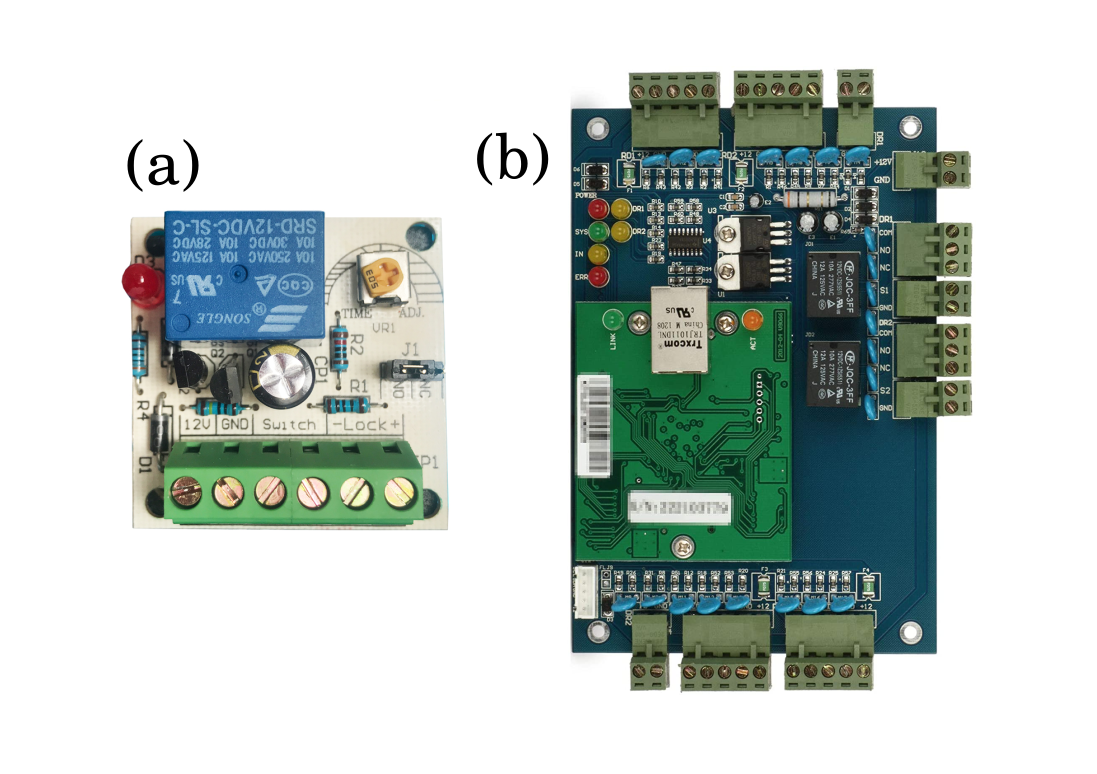
\includegraphics[width=0.7\textwidth]{Pictures/controladoras_simple_compleja.png}
	\rule{35em}{1pt}
	\caption[Controladoras Comparativa]{Controladoras de cerramientos eléctrico, a la izquierda un simple adaptador de voltaje a la derecha una central de acceso con múltiples puertos. }
	\label{fig:controladoras_simple_compleja}
\end{figure}
\subsection{Conexión con los controladores}
Del análisis y la comparación de los distintos tipos de controladores se pudo inferir el diseño general de estos sistemas así como sus componentes principales y accesorios que se listan a continuación:

\textbf{PRINCIPALES}
\begin{itemize}
	\item Etapa de Potencia y Adaptación de Voltajes 
	\item Driver Señal de Cerramiento
	\item Borneras para Cerramientos
	\item Bornera Pulsador Externo
	\item Microcontrolador y Firmware
\end{itemize}
\textbf{ACCESORIOS}
\begin{itemize}
	\item Bornera Luz Testigo Externa
	\item Bornera Barrera Infrarroja
	\item Bocina
	\item LEDs de Funcionamiento
	\item Pantalla
	\item Teclado
	\item Conmutadores Deslizantes de Configuración (DIP Switch)
	\item Jumpers de Configuración
	\item Pulsadores de Configuración
	\item Sensores Funcionamiento y Estado
	\item Módulo portero telefónico o Intercom
	\item Módulo RX RF para control remoto
	\item Lector etiquetas RFID
	\item Sensor Huella dactilar
\end{itemize}
En la Figura ~\ref{fig:controller_bdd} se puede observar un diagrama de definición por bloques del diseño generalizado para las controladoras de cerramientos eléctricos. Se resalta en violeta el componente correspondiente al pulsador físico externo.\\
\begin{figure}[htbp]
	\centering
	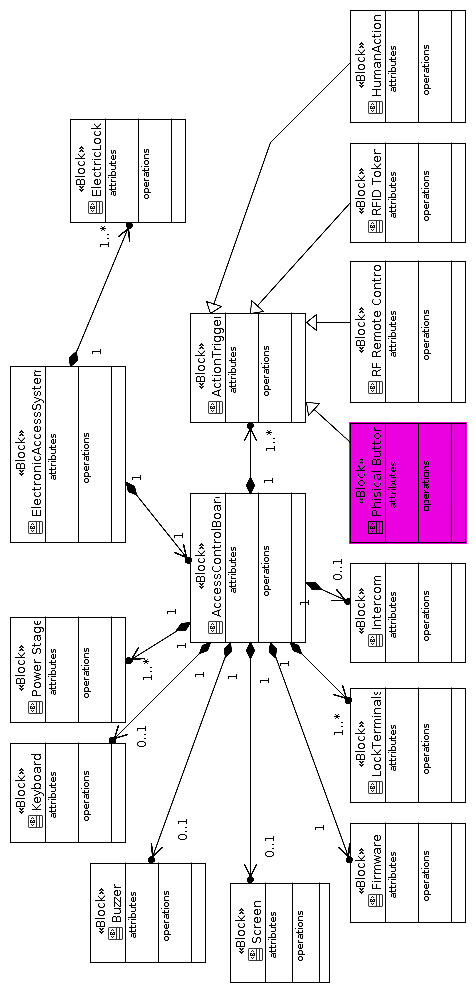
\includegraphics[width=0.6\textwidth]{Pictures/controller_bdd_baw_gimp.png}
	\rule{35em}{1pt}
	\caption[Diagrama Bloques Controlador]{Diagrama de definición por bloques para la generalización del diseño de los controladores.}
	\label{fig:controller_bdd}
\end{figure}
En el diagrama de bloques interno del controlador de la Figura ~\ref{fig:ibd_controladora} la señal de activación del pulsador es procesada por el módulo disparador de acciones que, en la mayoría de los casos, genera la señal de apertura o cierre según sea el estado del cerramiento.\\
\begin{figure}[htbp]
	\centering
	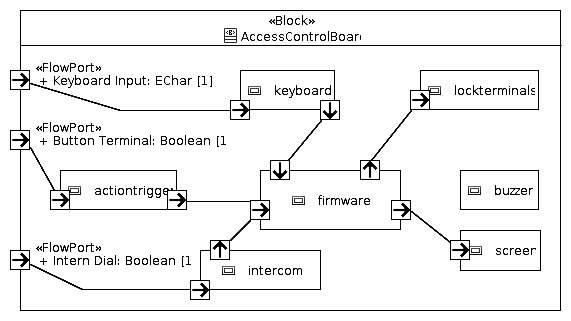
\includegraphics[width=0.8\textwidth]{Pictures/IBD_controladora_bw_gimp.png}
	\rule{35em}{1pt}
	\caption[Diagrama Bloques Internos Controlador]{Diagrama de bloques internos del diseño generalizado de un controlador de cerramientos eléctricos.}
	\label{fig:ibd_controladora}
\end{figure}
Después de realizar el análisis de los diseños se pudo evidenciar que la bornera para pulsador o botón externo es un factor común entre todos los modelos. Teniendo en cuenta esta particularidad se decidió adoptar esa interfaz de accionamiento como el modo de conexión universal de la solución a ser implementada. En la Figura ~\ref{fig:componentes_controladora+sol} se muestra un diagrama de componentes de alto nivel dónde se ilustra tal decisión.
\begin{figure}[htbp]
	\centering
	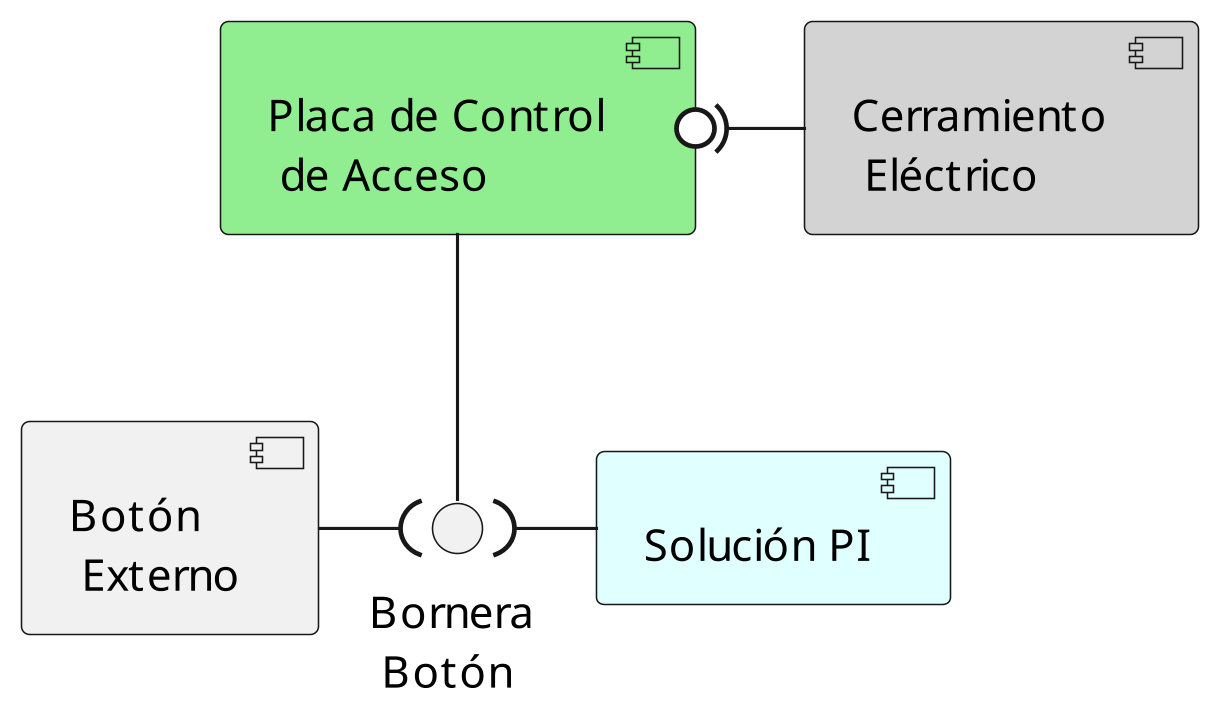
\includegraphics[width=0.6\textwidth]{Pictures/COMP_electric_locks.png}
	\rule{35em}{1pt}
	\caption[Diagrama de Componentes Conexión al Controlador]{Diagrama de componentes de alto nivel muestra la conexión propuesta para la solución de hardware.}
	\label{fig:componentes_controladora+sol}
\end{figure}
\section{Funcionalidades de un Sistema de Acceso}
Estos sistemas ofrecen la posibilidad de limitar el acceso a ciertas áreas de un inmueble mediante el control de cerramientos eléctricos utilizando llaves electrónicas u otros modos de autenticación de usuarios como sensores biométricos o el ingreso de credenciales por teclados. Para poder llevar a cabo esta tarea es primordial que estos controladores implementen una interfaz de configuración que permita entre otras operaciones:
\begin{itemize}
	\item Permitir la configuración del sistema utilizando una clave maestra.
	\item Dar de alta llaves electrónicas, nuevas credenciales biométricas o por teclado.
	\item Dar de baja llaves electrónicas, credenciales biométricas o por teclado.
	\item Resetear el sistema a sus valores de fábrica.
\end{itemize}
\section{Casos de Uso}
\label{section:casos_de_uso}
Teniendo en cuenta las funcionalidades básicas de un sistema de acceso tradicional y su adaptación a la propuesta de valor del producto se plantean los actores y casos de uso. %en la figura ~\ref{fig:USO_todos}.
Se identifican 5 actores que intervienen en el uso del producto: el \emph{Usuario} y sus 3 subtipos: \emph{Administrador, Autorizado e Invitado} y el \emph{Módulo Electrónico} que ejecutará los comandos recibidos previa autenticación y autorización.
En las figuras ~\ref{fig:uso_listado}, ~\ref{fig:uso_config}, ~\ref{fig:uso_usuarios} y ~\ref{fig:uso_rapido} se muestran los diagramas de casos de uso separados en paquetes para facilitar su lectura.
\begin{figure}[htbp]
	\centering
	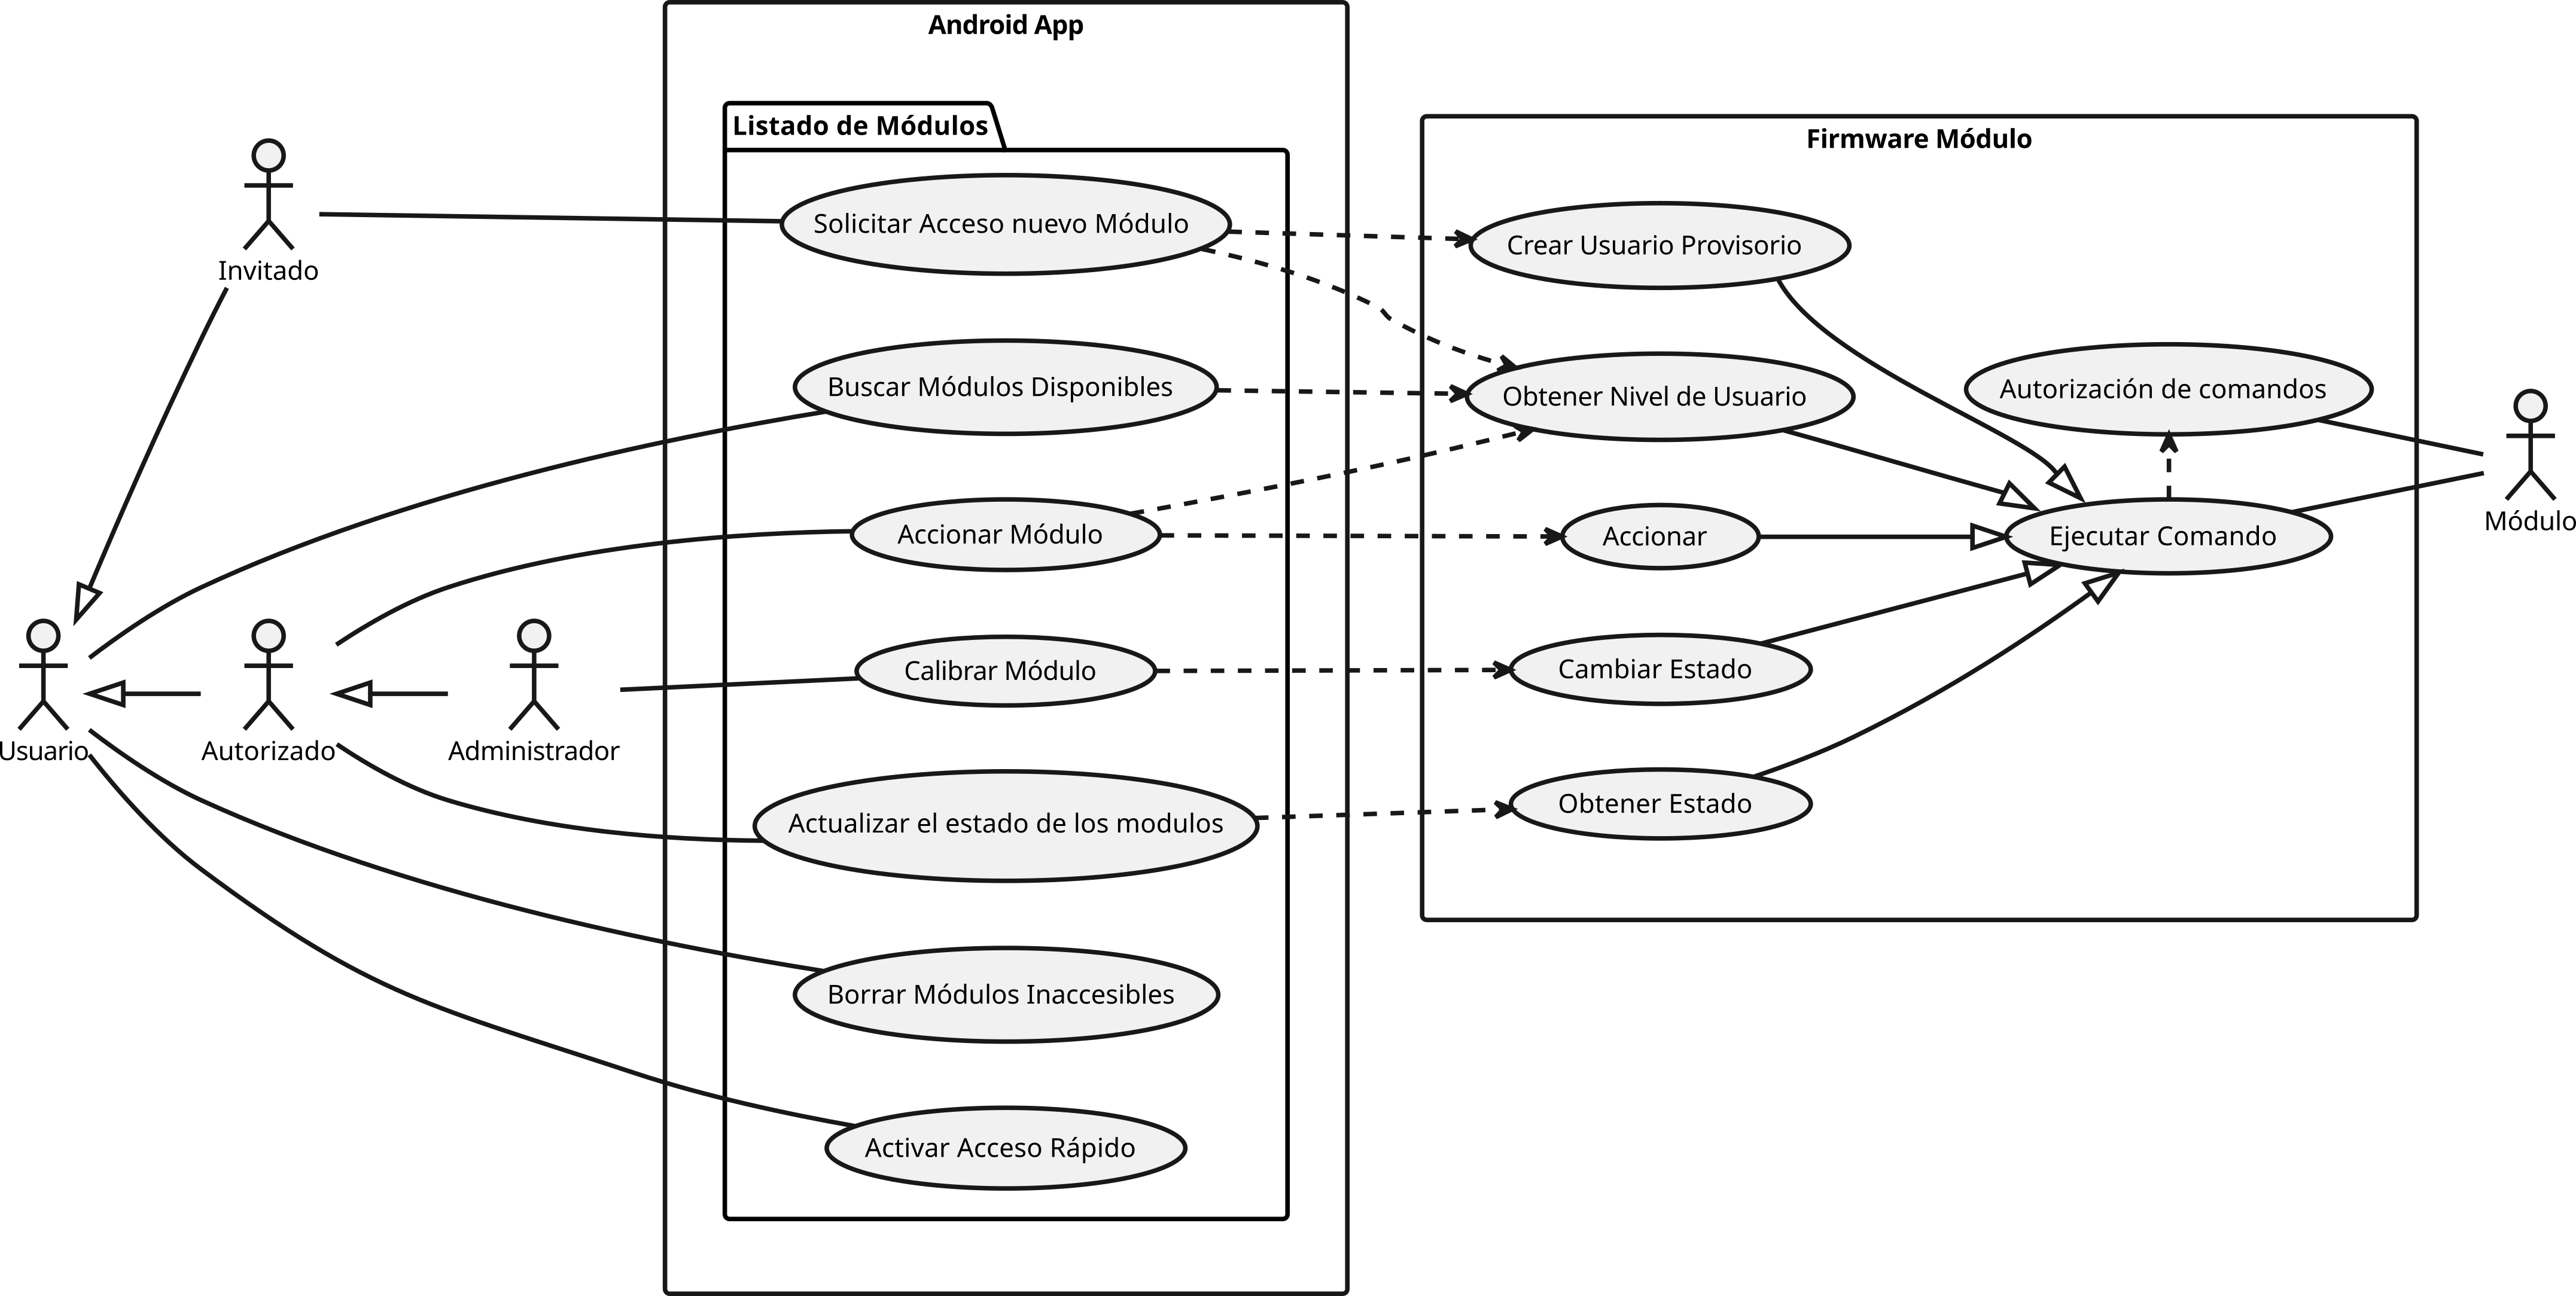
\includegraphics[width=\textwidth]{Figures/reque/USE_listado.png}
	\rule{35em}{1pt}
	\caption[Diagrama de Casos de Uso I]{Diagrama de casos de uso relacionados con el descubrimiento y control de módulos.}
	\label{fig:uso_listado}
\end{figure}

\begin{figure}[htbp]
	\centering
	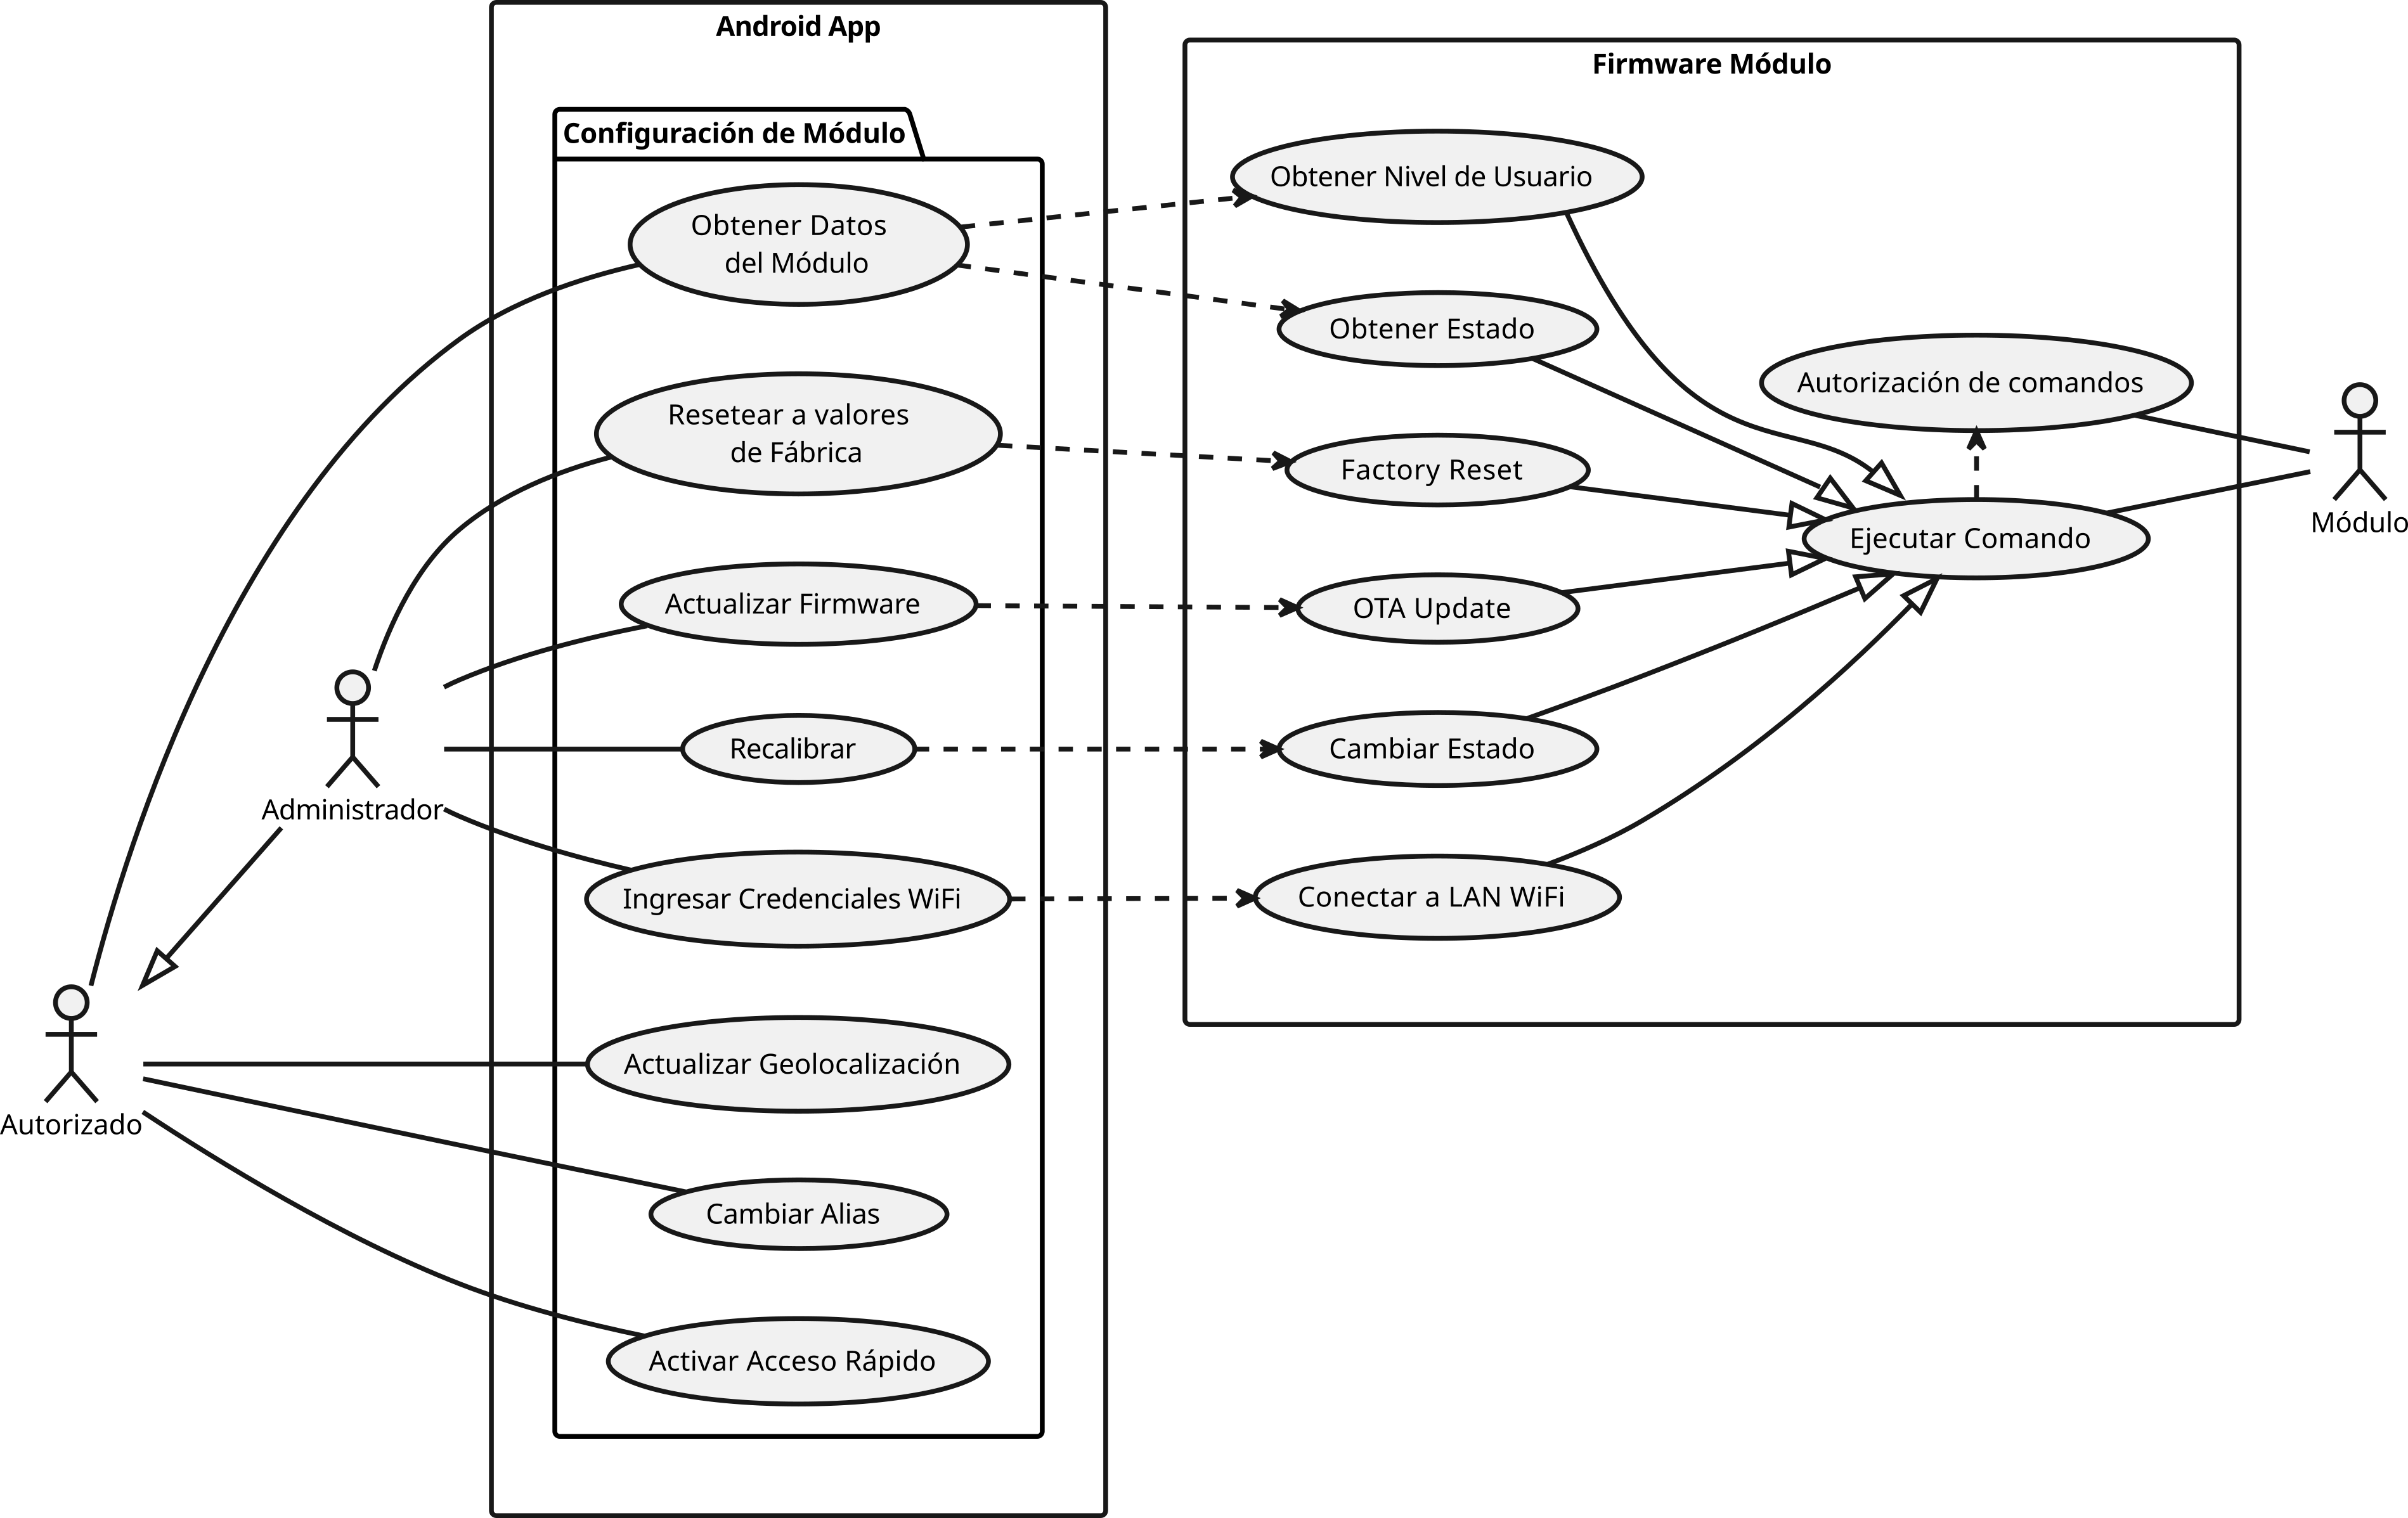
\includegraphics[width=\textwidth]{Figures/reque/USE_config.png}
	\rule{35em}{1pt}
	\caption[Diagrama de Casos de Uso II]{Diagrama de casos de uso relacionados con la configuración de un módulo.}
	\label{fig:uso_config}
\end{figure}

\begin{figure}[htbp]
	\centering
	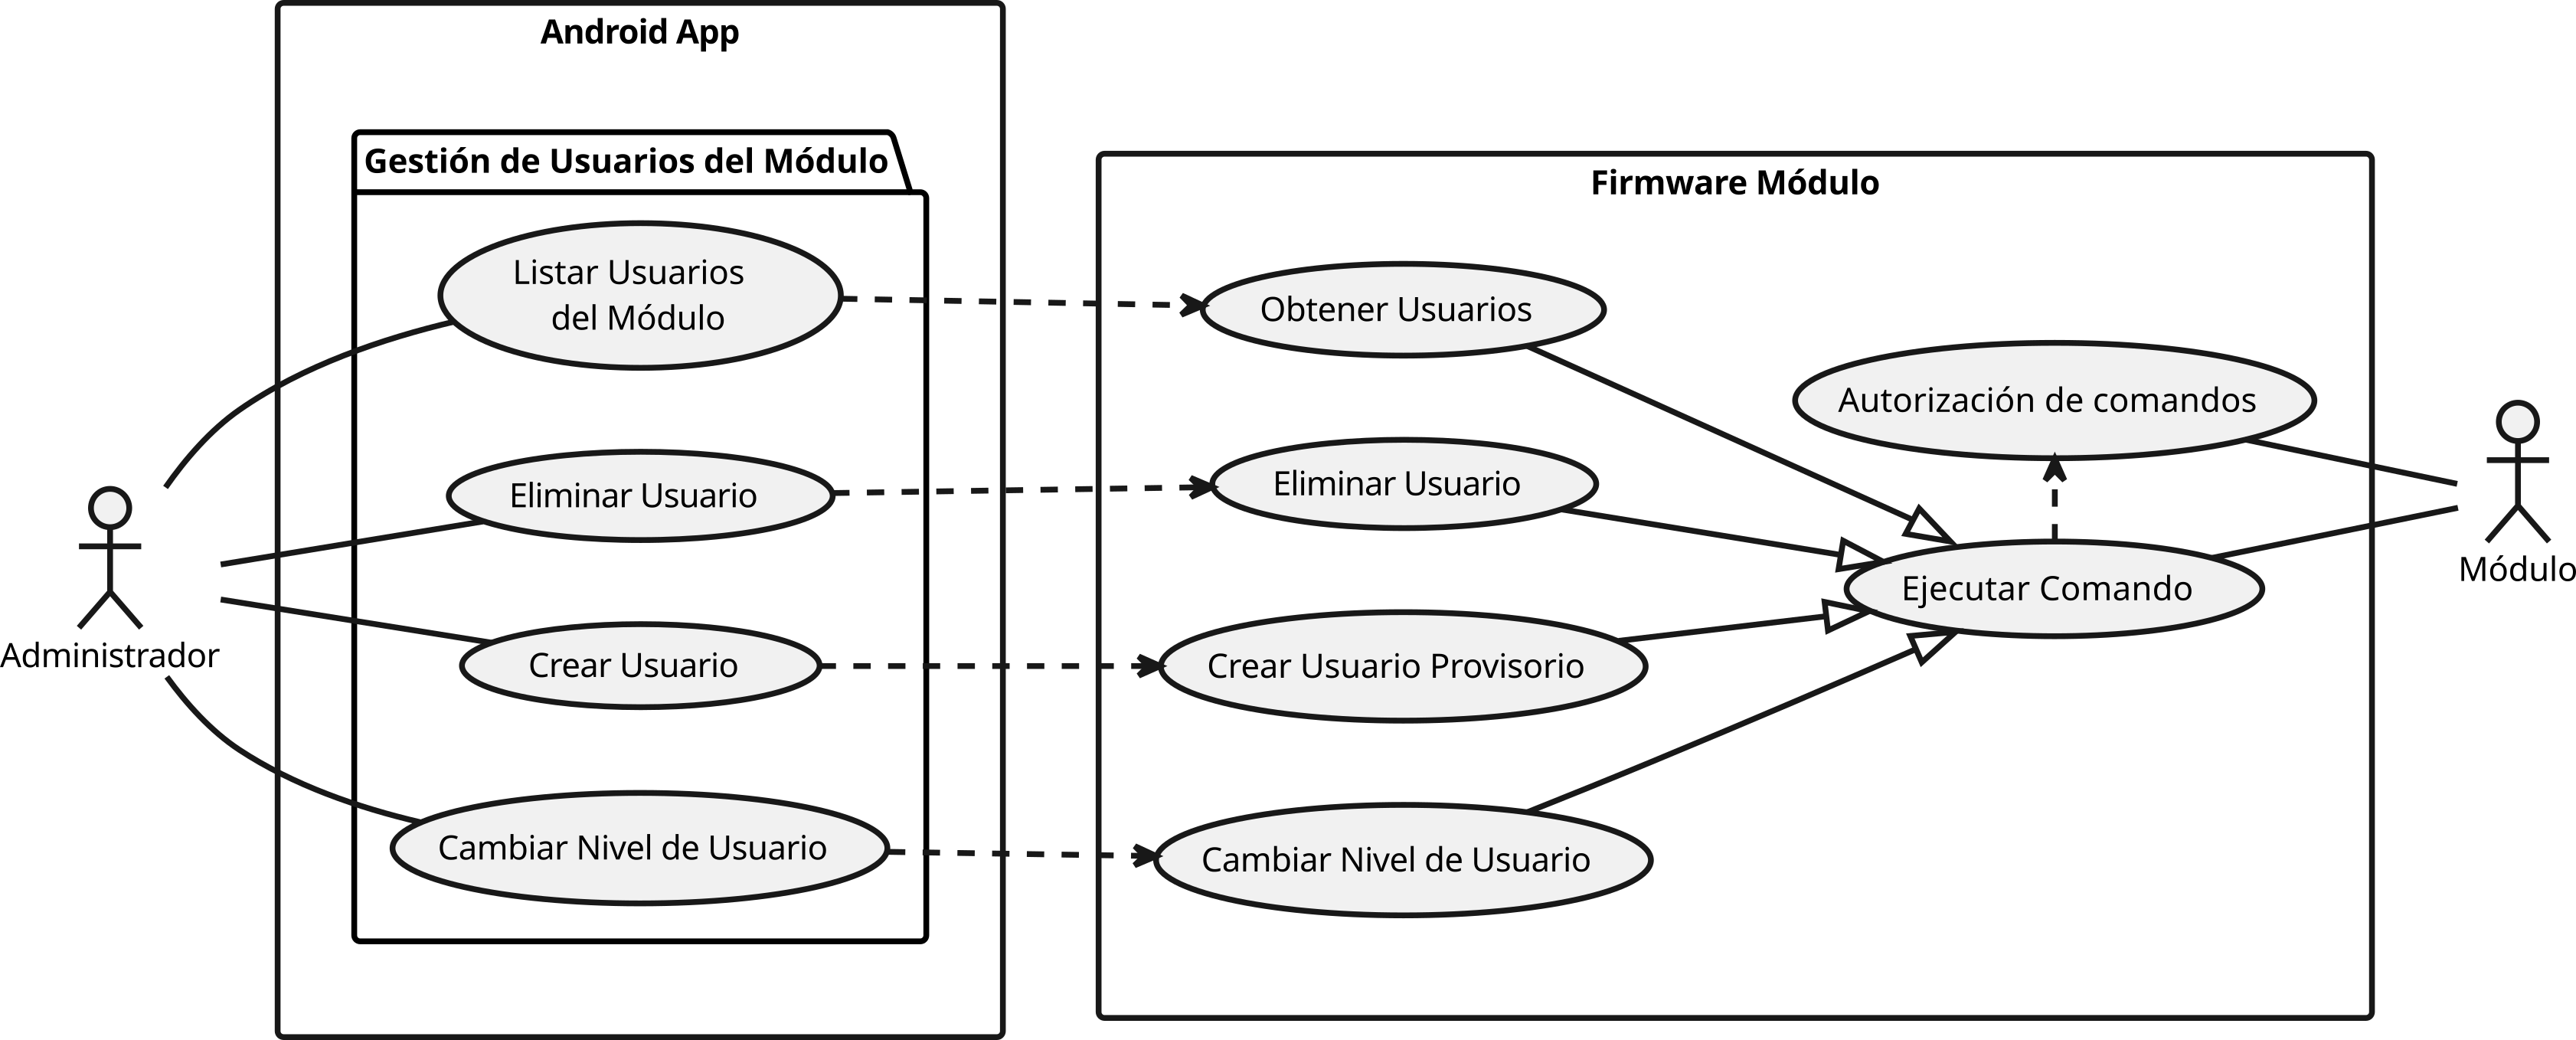
\includegraphics[width=\textwidth]{Figures/reque/USE_usuarios.png}
	\rule{35em}{1pt}
	\caption[Diagrama de Casos de Uso III]{Diagrama de casos de uso relacionados con el descubrimiento y control de módulos.}
	\label{fig:uso_usuarios}
\end{figure}

\begin{figure}[htbp]
	\centering
	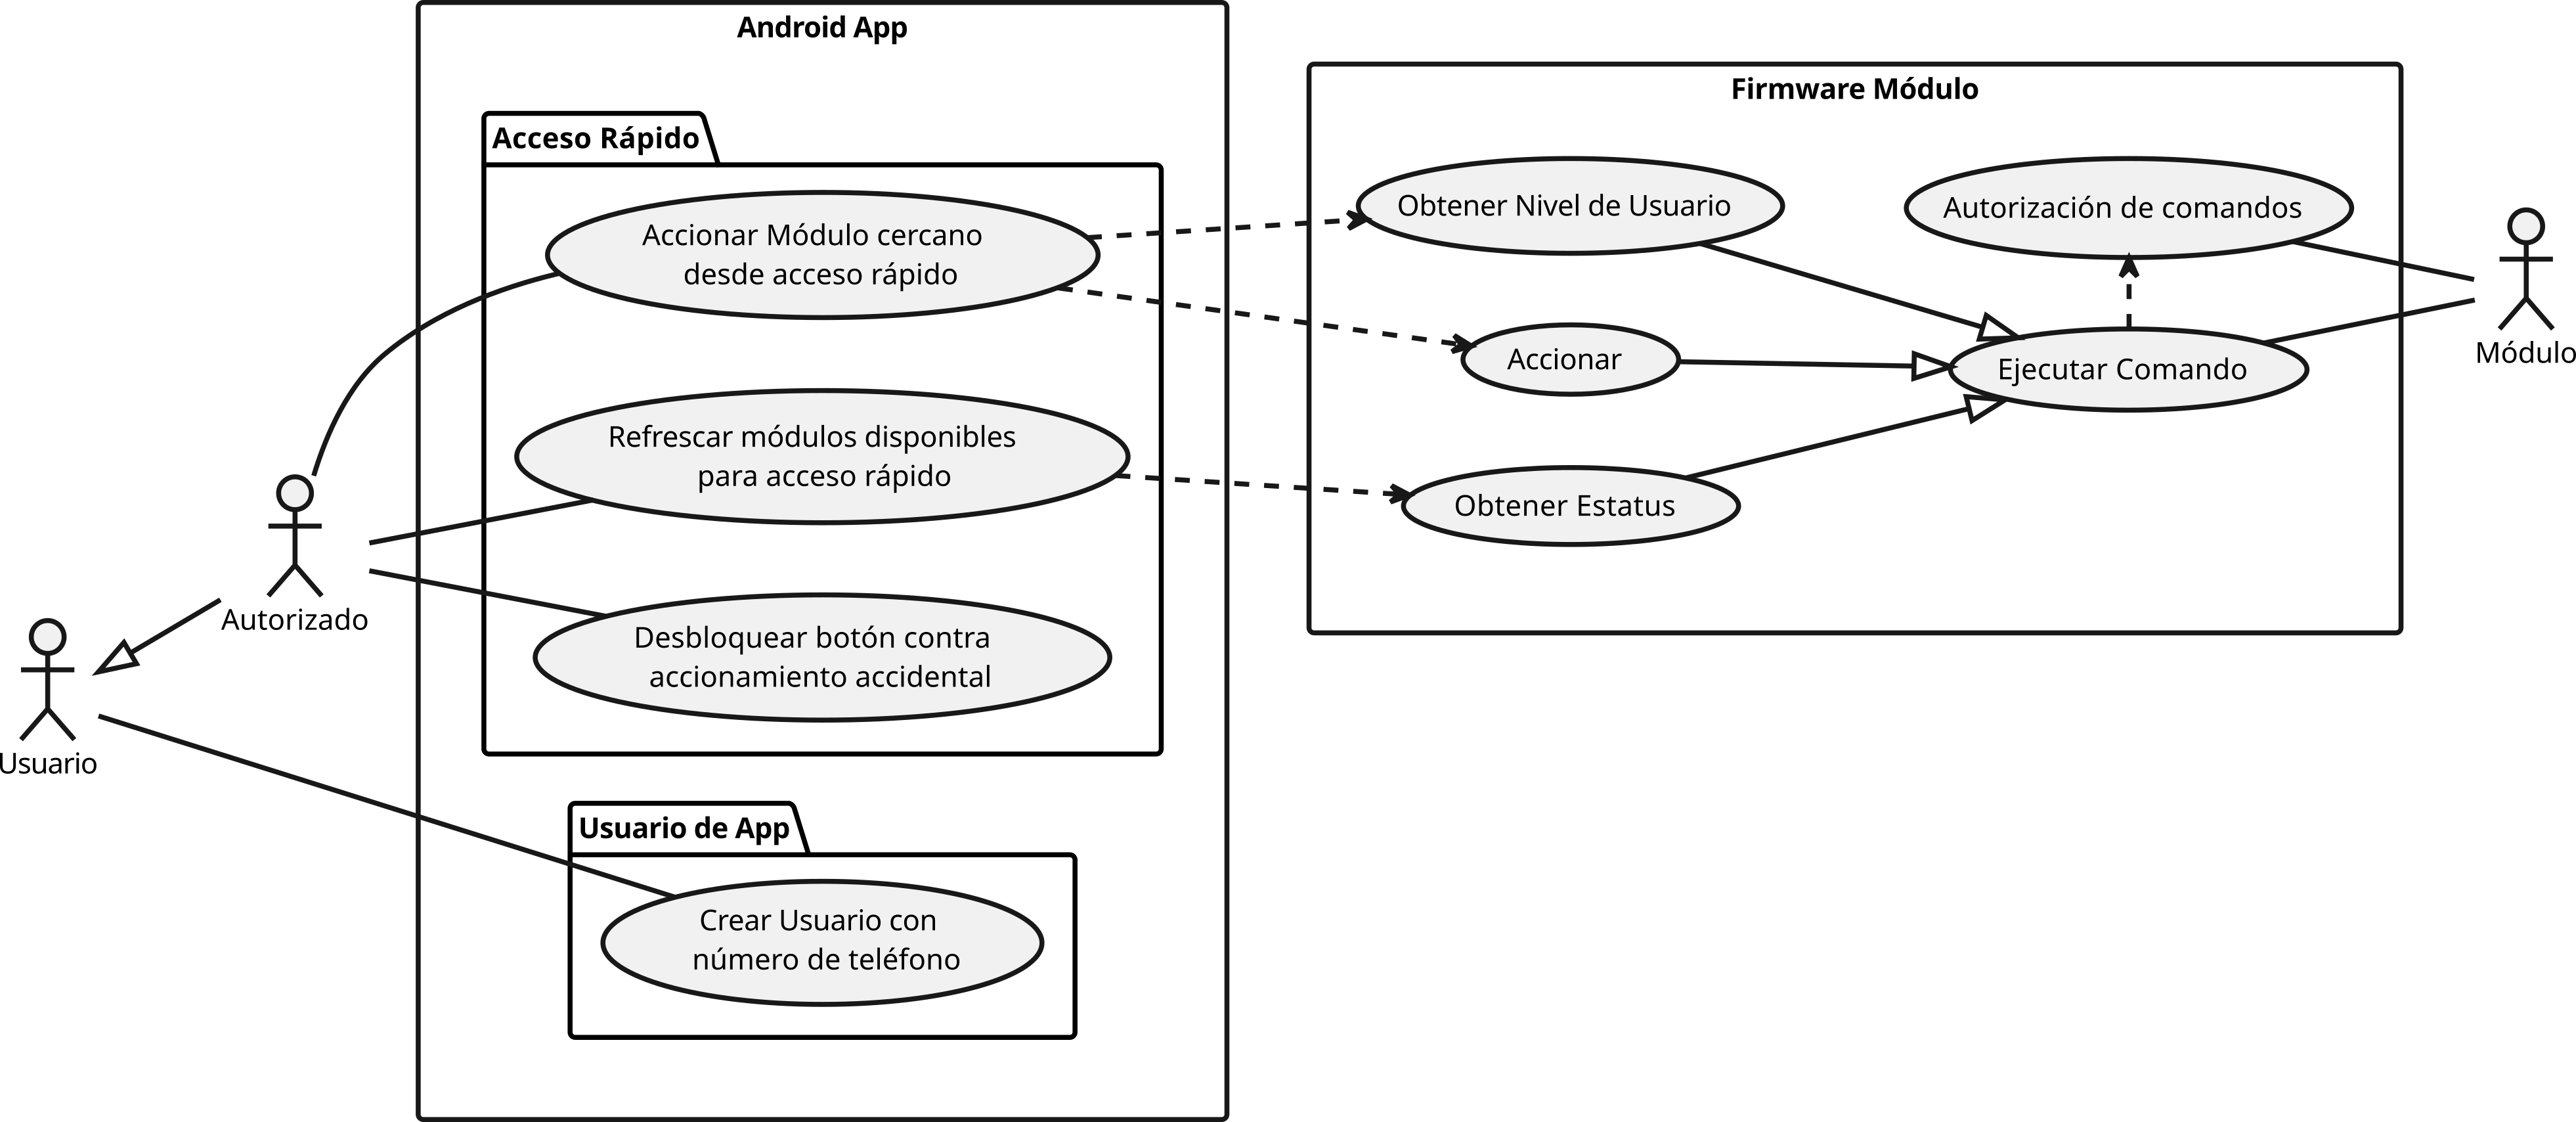
\includegraphics[width=\textwidth]{Figures/reque/USE_rapido.png}
	\rule{35em}{1pt}
	\caption[Diagrama de Casos de Uso IV]{Diagrama de casos de uso relacionados con el control rápido y el registro del usuario de la aplicación.}
	\label{fig:uso_rapido}
\end{figure}

\section{Requerimientos}
Considerando los casos de uso y el modo de conexión universal elegido se listan a continuación los requerimientos a nivel sistema de la solución propuesta.
\subsection{Requerimientos de Sistema}
A nivel de sistema se listan los requerimientos identificados en la Tabla ~\ref{table:req_sistemas}.
\begin{table}[ht]
	\centering
	%\resizebox{\textwidth}{!}{
	\begin{tabular}{|l|m{12cm}|}
		\hline
		\textbf{ID} & \textbf{Descripción}                                                                                             \\ \hline
		RS00        & El sistema debe accionar cerramientos eléctricos.                                                                \\ \hline
		RS01        & El sistema debe permitir que un mismo usuario tenga acceso a múltiples cerramientos.                             \\ \hline
		RS02        & El sistema debe establecer conexión a la red wifi del inmueble donde será instalado.                             \\ \hline
		RS03        & El sistema debe mantenerse operativo offline de manera local.                                                    \\ \hline
		RS04        & El sistema debe funcionar de manera remota a través de internet.                                                 \\ \hline
		RS05        & El sistema debe admitir alta de nuevos usuarios para un cerramiento.                                             \\ \hline
		RS06        & El sistema debe permitir la baja de usuarios.                                                                    \\ \hline
		RS07        & El sistema debe permitir el cambio de privilegios de los usuarios.                                               \\ \hline
		RS08        & El sistema debe admitir la conexión y calibración de sensores (fin de carrera, encoder y de apertura magnética). \\ \hline
		RS09        & El sistema debe permitir su restablecimiento a valores de fábrica.                                               \\ \hline
		RS10        & El sistema debe permitir actualizar su versión de software de manera sencilla.                                   \\ \hline
	\end{tabular}
	%}
	\caption[Requerimientos de Sistema]{Tabla de requerimientos a nivel de sistema para la solución propuesta.}
	\label{table:req_sistemas}
\end{table}
\subsection{Modulo Electrónico}
Los requerimientos encontrados para el Módulo Electrónico se listan en la Tabla ~\ref{table:req_modulo_electro}.
Estos requerimientos fueron implementados por un colaborador del equipo quién se encargó principalmente del desarrollo del firmware por lo que los detalles del diseño y la implementación del software embebido exceden los alcances de este informe. 
\begin{table}[ht]
	\centering
	%\resizebox{\textwidth}{!}{
	\begin{tabular}{|c|m{12cm}|}
		\hline
		\textbf{ID} & \multicolumn{1}{c|}{\textbf{Descripción}}                                                                                    \\ \hline
		RME00       & El módulo electrónico debe alimentarse con 220v AC.                                                                          \\ \hline
		RME01       & El módulo electrónico debe conectarse al controlador por la bornera de pulsador externo                                      \\ \hline
		RME02       & El módulo electrónico debe conectarse a la red wifi del inmueble donde será instalado.                                       \\ \hline
		RME03       & El módulo electrónico debe almacenar los usuarios registrados autorizados para                                               \\ \hline
		RME04       & El módulo electrónico debe funcionar de manera remota a través de internet.                                                  \\ \hline
		RME05       & El módulo electrónico debe funcionar de manera local offline en caso de que la conexión a internet se vea interrumpida.      \\ \hline
		RME06       & El módulo electrónico debe recibir comandos desde la aplicación cliente y devolver una respuesta según se detalla en la API. \\ \hline
		RME07       & El módulo electrónico debe contar con puertos para los distintos tipos de sensores.                                          \\ \hline
		RME08       & El módulo electrónico debe contar con luces indicadoras de funcionamiento.                                                   \\ \hline
		RME09       & El módulo electrónico debe incluir botones para configuración y operación.                                                   \\ \hline
		RME10       & El módulo electrónico debe poder actualizar su versión de firmware de manera inalámbrica.                                    \\ \hline
	\end{tabular}
	%}
	\caption[Requerimientos del Módulo Electrónico]{Tabla de requerimientos del Módulo Electrónico.}
	\label{table:req_modulo_electro}
\end{table}
\subsection{Aplicación Móvil}
En la tabla ~\ref{table:req_aplicacion} se listan los requerimientos encontrados para la aplicación móvil.
\begin{table}[ht]
	\centering
	%\resizebox{\textwidth}{!}{
	\begin{tabular}{|l|m{12cm}|}
		\hline
		\multicolumn{1}{|c|}{\textbf{ID}} & \multicolumn{1}{c|}{\textbf{Descripción}}                                                                 \\ \hline
		RA00                              & La aplicación debe permitir el registro inicial del usuario con su número de teléfono.                    \\ \hline
		RA01                              & La aplicación debe generar una clave única y secreta para el envío de comandos.                           \\ \hline
		RA02                              & La aplicación debe descubrir y listar módulos electrónicos nuevos y ya configurados.                      \\ \hline
		RA03                              & La aplicación debe permitir enviar comandos al módulo y recibir la respuestas según se detalla en la API. \\ \hline
		RA04                              & La aplicación debe permitir configurar los módulos nuevos.                                                \\ \hline
		RA05                              & La aplicación debe permitir solicitar acceso a los módulos electrónicos encontrados ya configurados.      \\ \hline
		RA06                              & La aplicación debe permitir el accionamiento de los cerramientos eléctricos.                              \\ \hline
		RA07                              & La aplicación debe permitir cambiar el alias de los módulos.                                              \\ \hline
		RA08                              & La aplicación debe ofrecer un modo de accionamiento con pantalla bloqueada.                               \\ \hline
		RA09                              & La aplicación debe ofrecer distintas configuraciones según el privilegio del usuario.                     \\ \hline
		RA10                              & La aplicación debe permitir al usuario administrador restablecer el módulo a valores de fábrica.          \\ \hline
		RA11                              & La aplicación debe permitir al usuario administrador calibrar el sensor.                                  \\ \hline
		RA12                              & La aplicación debe permitir al usuario administrador invitar a nuevos usuarios.                           \\ \hline
		RA13                              & La aplicación debe permitir al usuario administrador convertir usuarios a administradores.                \\ \hline
		RA14                              & La aplicación debe permitir al usuario administrador eliminar cualquier usuario.                          \\ \hline
		RA15                              & La aplicación debe permitir al usuario administrador actualizar la versión del firmware del módulo.       \\ \hline
	\end{tabular}
	\caption[Requerimientos de la Aplicación]{Tabla de requerimientos de la Aplicación Cliente.}
	\label{table:req_aplicacion}
	%	}
\end{table}



\subsection{Identificación de Riesgos}

En esta sección se expone el panorama de incertidumbres del proyecto y se hace foco en las eventualidades que pueden surgir durante su ejecución. Estas pueden alterar, de alguna manera, la planificación y duración del proyecto.
La gestión temprana de riesgos facilita la identificación de los mismos y permite la creación de planes de contingencia para minimizar el efecto en caso de ocurrencia.

Las situaciones que puedan constituir una amenaza a la realización del proyecto se pueden clasificar por el objeto de impacto o por su causalidad.

Categorización por objeto de impacto.
\begin{itemize}
	\item Al Proyecto: afectan la planificación y los recursos del proyecto.
	\item Al Producto: afectan la calidad o el rendimiento del producto.
	\item Al Negocio: afectan a la organización que desarrolla el producto.
\end{itemize}


Por otro lado se pueden clasificar los riesgos respecto de su origen o causa.

\begin{itemize}
	\item \textbf{Riesgo Tecnológico} (TECNO): Estrechamente relacionado con los aspectos técnicos del proyecto se evidencian en las herramientas utilizadas para la implementación, evaluación y ejecución del trabajo. En el caso del presente proyecto existirán riesgos de hardware y software.
	\item \textbf{Riesgo de Personal} (PER) : Relacionados a las personas involucradas en la ejecución del proyecto. En este caso el equipo de desarrollo.
	\item \textbf{Riesgo Organizacional}(ORG): Derivan del entorno dónde se está realizando el trabajo. En este caso el proyecto está vinculado a un emprendimiento tecnológico.
\end{itemize}

\subsection{Análisis de Riesgo}
Para poder tener un panorama completo de los riesgos del proyecto se elabora una tabla con los riesgos identificados y se pondera de manera cualitativa los mismos. Los parámetros de esta ponderación serán la probabilidad de ocurrencia y el impacto de su efecto.\\
\textbf{La probabilidad de ocurrencia} se estimará en tres valores: Improbable (0.3), Probable (0.6) y Muy Probable (0.9).\\
\textbf{El impacto} se estimará también en tres valores: Bajo (1), Moderado(10), Alto(100)\\
Realizando el producto aritmético entre estos parámetros se calcula la importancia de los riesgos identificados como se puede observar en la Tabla ~\ref{table:riegos_identificados}.
Aunque el valor de importancia obtenido es ilustrativo ofrece una alternativa numérica que permite el ordenamiento y con esto un inmediato orden de prioridad.

\begin{table}[ht]
	%\centering
	%\resizebox{1\textwidth}{!}{
	\begin{tabular}{|c|>{\small}m{3cm}|m{5em}|c|c|c|c|}
		\hline
		\textbf{ID} & \multicolumn{1}{c|}{\textbf{Descripción}} & \textbf{\small{Objeto de Impacto}} & \textbf{Causa} & \textbf{Probabilidad} & \textbf{Impacto} & \textbf{Importancia} \\ \hline
		R00         & Problemas con el entendimiento de la arquitectura elegida para la implementacion & PROY                       & PER            & 0.3                   & 100              & 30                   \\ \hline
		R01         & Implementación de la arquitectura elegida                                        & PROY                       & PER            & 0.6                   & 100              & 60                   \\ \hline
		R02         & Entendimiento del paradigma de programacion reactiva utilizando RxJava           & PROY                       & PER            & 0.6                   & 10               & 6                    \\ \hline
		R03         & Cambio de versiones de librerias                                                 & PROY                       & TEC            & 0.6                   & 1                & 0.6                  \\ \hline
		R04         & Falta de librerías de comunicacion                                               & PROY                       & TEC            & 0.3                   & 100              & 30                   \\ \hline
		R05         & Librerias de comunicacion no adaptadas a programacion reactiva                   & PROY                       & TEC            & 0.6                   & 10               & 6                    \\ \hline
		R06         & Falta de documentación de las librerías                                          & PROY                       & TEC            & 0.9                   & 10               & 9                    \\ \hline
		R07         & Retraso o complicaciones en el desarrollo del módulo electrónico                 & PROY                       & PER            & 0.9                   & 100              & 90                   \\ \hline
		R08         & Subestimación de tiempo de desarrollo                                            & PROY                       & ORG            & 0.9                   & 10               & 9                    \\ \hline
		R09         & Cambio de requerimientos durante el deesarrollo                                  & PROY                       & NEG            & 0.9                   & 100              & 90                   \\ \hline
	\end{tabular}
	\caption[Riesgos Identificados]{Tabla de riesgos identificados y la ponderación para el cálculo de su importancia.}
	\label{table:riegos_identificados}
	%	}
\end{table}

\subsection{Planificación de Riesgos}
Con el objetivo de minimizar los efectos de las posibles eventualidades riesgosas se plantean tres tipos de estrategias que se detallan a continuación.

\begin{itemize}
	\item De Prevención: Acciones preventivas orientadas a reducir la probabilidad de ocurrencia.
	\item De Mitigación: Acciones preventivas orientadas a atenuar el impacto en caso de ocurrencia.
	\item De Contingencia: Acciones curativas en caso de ocurrencia.
\end{itemize}

Para los 5 riesgos identificados más importantes se plantearon las estrategias y se exponen en la Tabla ~\ref{table:planificacion_riesgos}.

\begin{table}[ht]
	%\centering
	%\resizebox{1\textwidth}{!}{
	\begin{tabular}{|c|>{\small}m{3cm}|>{\small}m{3cm}|>{\small}m{3cm}|>{\small}m{3.5cm}|}
		\hline
		\multirow{2}{*}{\textbf{ID}} & \multicolumn{1}{c|}{\multirow{2}{*}{\textbf{Descripción}}}                       & \multicolumn{3}{c|}{\textbf{Estrategia}}                                                                                                                                                                                                                                                                                                                                                                                                                                                                                           \\ \cline{3-5} 
		& \multicolumn{1}{c|}{}                                                            & \multicolumn{1}{c|}{\textbf{De Prevención}}                                                                                                                           & \multicolumn{1}{c|}{\textbf{De Mitigación}}                                                                                                                                  & \multicolumn{1}{c|}{\textbf{De Contingencia}}                                                                                                                               \\ \hline
		R06                          & Retraso o complicaciones en el desarrollo del módulo electrónico                 & Se iniciará el desarrollo de ambos componentes una vez que se hayan establecido las tecnologías para ambos.                                                           & Se establecerá con claridad una API de comunicación a modo de contrato y con una versión definida.                                                                           & Con las definiciones de la API se puede simular el comportamiento del módulo.                                                                                               \\ \hline
		R08                          & Cambio de requerimientos durante el desarrollo                                  & Se celebraran entrevistas con los posibles clientes y usuarios para anticipar cambios y requerimientos futuros.                                                       & Se realizará una revisión de los requerimientos periódica.                                                                                                                   & Se planificará la modificación o adición de funcionalidad para la próxima versión. Intentando mantener siempre un entregable funcional.                                       \\ \hline
		R01                          & Implementación de la arquitectura elegida                                        & Se buscarán ejemplos de implementaciones similares y documentación respaldatoria.                                                                                     & Se contará con el apoyo de algún contacto técnico externo con experiencia para poder consultar.                                                                              & Se agregarán la resolución de conflictos a la planificación de tareas ordinarias para tener en cuenta el impacto y el progreso en ese aspecto.                              \\ \hline
		R00                          & Problemas con el entendimiento de la arquitectura elegida para la implementación & Se recolectará bibliografía diversa sobre los conceptos introducidos con la arquitectura.                                                                             & Se podrá realizar consultas inter-equipo para despejar dudas y evitar retrasos.                                                                                              & Se pondrá en marcha un pequeño análisis de impacto al reemplazar el asunto bloqueante por una alternativa más sencilla y quedará documentado.                               \\ \hline
		R03                          & Falta de librerías de comunicación                                               & Se escogerá un framework de desarrollo lo suficientemente maduro como para anticipar la búsqueda de las librerías necesarias. Y asegurar la existencia de las mismas. & Se empleará un modo de implementación por interfaces a modo Mock, de manera que se pueda postergar el uso de la biblioteca sin retrasar el desarrollo de las funcionalidades & Se buscarán alternativas a los protocolos originalmente propuestos y se evaluará el impacto sobre la implementación. En caso de ser un cambio viable se dejará documentado. \\ \hline
	\end{tabular}
	\caption[Planificación de Riesgos]{Tabla con la planificación de los riesgos más importantes.}
	\label{table:planificacion_riesgos}
	%}
\end{table}




%% Chapter Template

\chapter{Diseño} % Main chapter title

\label{Chapter4} % Change X to a consecutive number; for referencing this chapter elsewhere, use \ref{ChapterX}

\lhead{Capítulo  4. \emph{Diseño}} % Change X to a consecutive number; this is for the header on each page - perhaps a shortened title

%----------------------------------------------------------------------------------------
%	SECTION 1
%----------------------------------------------------------------------------------------
\section{Dominio del Problema}
Como se detalló en la Sección ~\ref{section:controladores} todos los cerramientos eléctricos no funcionan por sí solos sino que necesitan de un controlador. Estos controladores se comercializan en diferentes presentaciones con distintos diseños, desde simples interfaces eléctricas para un botón pulsador externo como se muestra en la Figura ~\ref{fig:controladoras_simple_compleja}(a) hasta complejas centrales de acceso electrónico como la que se muestra en la Figura ~\ref{fig:controladoras_simple_compleja}(b) que incluyen interfaces para sistemas de identificación de usuarios o soporte para llaves electrónicas descritas en la Sección ~\ref{section:llaves_electronicas}.
\begin{figure}[htbp]
	\centering
	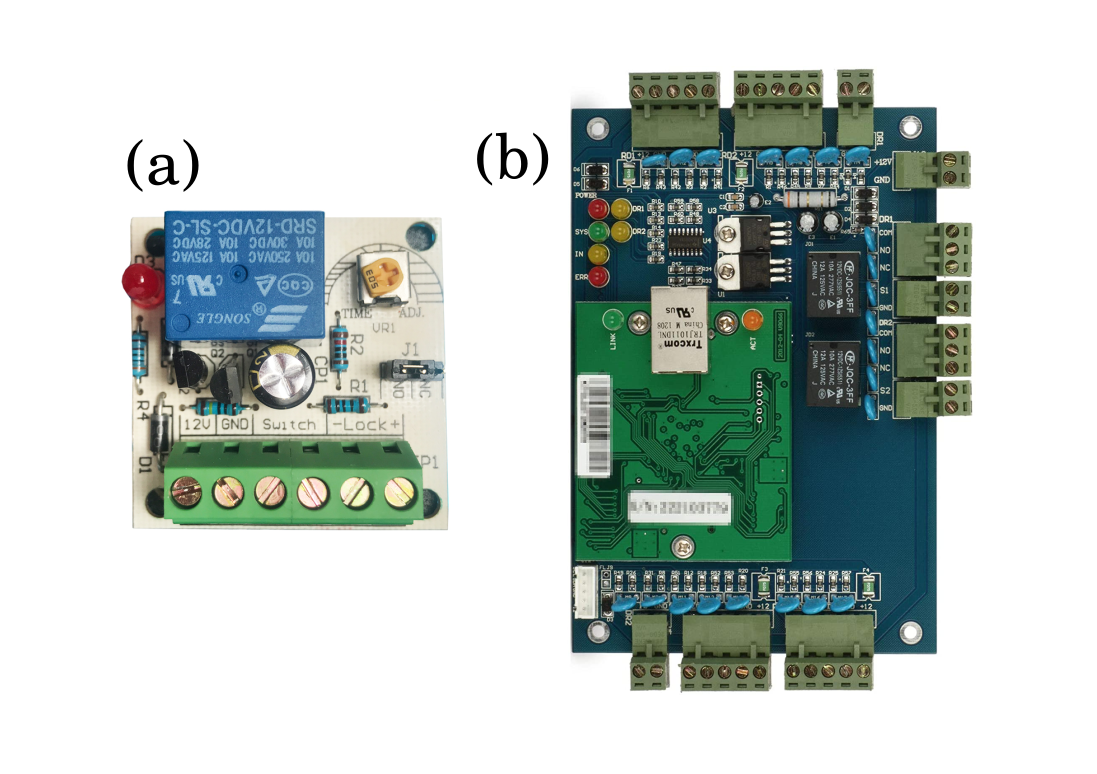
\includegraphics[width=0.6\textwidth]{Pictures/controladoras_simple_compleja.png}
	\rule{35em}{1pt}
	\caption[Controladoras Comparativa]{Controladoras de cerramientos eléctrico, a la izquierda un simple adaptador de voltaje a la derecha una central de acceso con múltiples puertos. }
	\label{fig:controladoras_simple_compleja}
\end{figure}
\subsection{Conexión con los controladores}
Del análisis y la comparación de los distintos tipos de controladores se pudo inferir el diseño general de estos sistemas así como sus componentes principales y accesorios que se listan a continuación:\\
\textbf{PRINCIPALES}
\begin{itemize}
	\item Etapa de Potencia y Adaptación de Voltajes 
	\item Driver Señal de Cerramiento
	\item Borneras para Cerramientos
	\item Bornera Pulsador Externo
	\item Microcontrolador y Firmware
\end{itemize}
\textbf{ACCESORIOS}
\begin{itemize}
	\item Bornera Luz Testigo Externa
	\item Bornera Barrera Infrarroja
	\item Bocina
	\item LEDs de Funcionamiento
	\item Pantalla
	\item Teclado
	\item Conmutadores Deslizantes de Configuración (DIP Switch)
	\item Jumpers de Configuración
	\item Pulsadores de Configuración
	\item Sensores Funcionamiento y Estado
	\item Módulo portero telefónico o Intercom
	\item Módulo RX RF para control remoto
	\item Lector etiquetas RFID
	\item Sensor Huella dactilar
\end{itemize}
En la Figura ~\ref{fig:controller_bdd} se puede observar un diagrama de definición por bloques del diseño generalizado para las controladoras de cerramientos eléctricos. Se resalta en violeta el componente correspondiente el pulsador físico externo.\\
\begin{figure}[htbp]
	\centering
	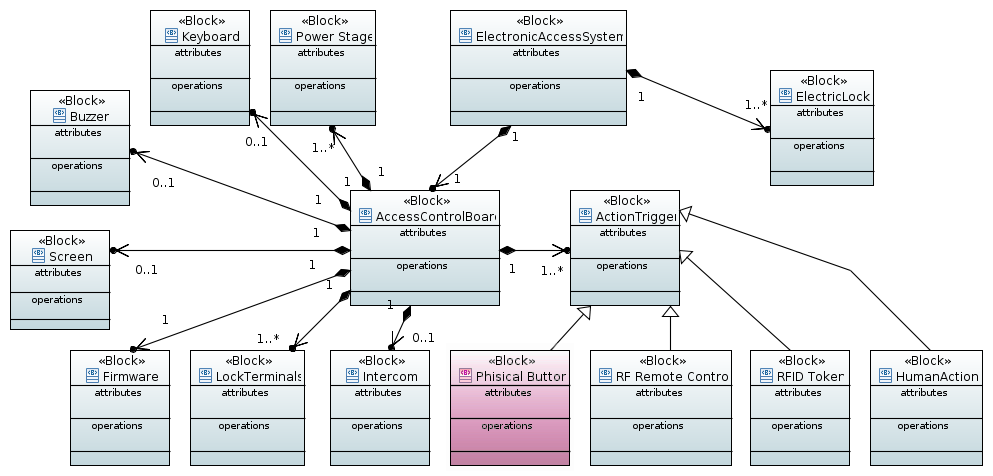
\includegraphics[width=0.9\textwidth]{Pictures/controller_bdd.png}
	\rule{35em}{1pt}
	\caption[Diagrama Bloques Controlador]{Diagrama de definición por bloques para la generalización del diseño de los controladores.}
	\label{fig:controller_bdd}
\end{figure}
En el diagrama de bloques interno del controlador de la Figura ~\ref{fig:ibd_controladora} la señal de activación del pulsador es procesada por el módulo de disparador de acciones en la mayoría de los casos generando la señal de apertura o cierre del cerramiento según sea el estado del mismo.\\
\begin{figure}[htbp]
	\centering
	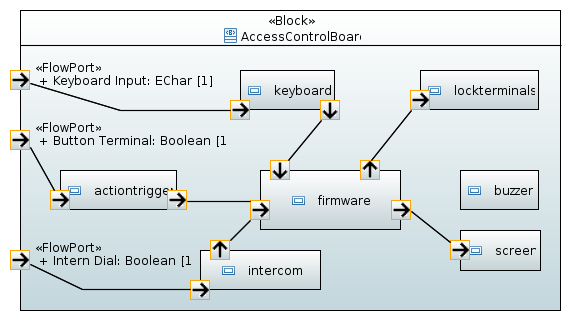
\includegraphics[width=0.6\textwidth]{Pictures/IBD_controladora.png}
	\rule{35em}{1pt}
	\caption[Diagrama Bloques Internos Controlador]{Diagrama de bloques internos del diseño generalizado de un controlador de cerramientos eléctricos.}
	\label{fig:ibd_controladora}
\end{figure}
Después de realizar el análisis de los diseños se pudo evidenciar que la bornera para pulsador o botón externo es un factor común entre todos los modelos. Teniendo en cuenta esta particularidad se decidió adoptar esta interfaz de accionamiento como el modo de conexión universal de la solución a ser implementada. En la Figura ~\ref{fig:componentes_controladora+sol} se muestra un diagrama de componentes de alto nivel dónde se ilustra tal decisión.
\begin{figure}[htbp]
	\centering
	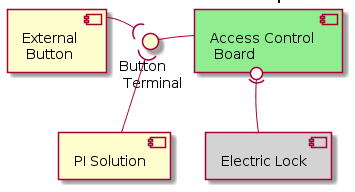
\includegraphics[width=0.5\textwidth]{Pictures/componentes_controladora+sol.png}
	\rule{35em}{1pt}
	\caption[Diagrama de Componentes Conexión al Controlador]{Diagrama de componentes de alto nivel muestra la conexión propuesta para la solución de hardware.}
	\label{fig:componentes_controladora+sol}
\end{figure}
\subsection{Funcionalidades básicas de un Sistema de Acceso}
Estos sistemas ofrecen la posibilidad de limitar el acceso a ciertas áreas de un inmueble mediante el control de cerramientos eléctricos utilizando llaves electrónicas u otros modos de autenticación de usuarios como sensores biométricos o el ingreso de credenciales por teclados. Para poder llevar a cabo esta tarea es primordial que estos controladores implementen una interfaz de configuración que permita entre otras operaciones:
\begin{itemize}
	\item Permitir la configuración del sistema utilizando una clave maestra.
	\item Dar de alta llaves electrónicas, nuevas credenciales biométricas o por teclado.
	\item Dar de baja llaves electrónicas, credenciales biométricas o por teclado.
	\item Resetear el sistema a sus valores de fábrica.
\end{itemize}
\section{Requerimientos}
Considerando las funcionalidades básicas de un sistema de acceso tradicional y el modo de conexión universal elegido se listan a continuación los requerimientos a nivel sistema de la solución propuesta.
\subsection{Requerimientos a nivel de Sistema}
A nivel de sistema se listan los requerimientos identificados en la Tabla ~\ref{table:req_sistemas}.
\begin{table}[ht]
	%\centering
	%\resizebox{\textwidth}{!}{
		\begin{tabular}{|l|m{12cm}|}
			\hline
			\textbf{ID} & \textbf{Descripción}                                                                                             \\ \hline
			RS00        & El sistema debe accionar cerramientos eléctricos.                                                                \\ \hline
			RS01        & El sistema debe permitir que un mismo usuario tenga acceso a múltiples cerramientos.                             \\ \hline
			RS02        & El sistema debe establecer conexión a la red wifi del inmueble donde será instalado.                             \\ \hline
			RS03        & El sistema debe mantenerse operativo offline de manera local.                                                    \\ \hline
			RS04        & El sistema debe funcionar de manera remota a través de internet.                                                 \\ \hline
			RS05        & El sistema debe admitir alta de nuevos usuarios para un cerramiento.                                             \\ \hline
			RS06        & El sistema debe permitir la baja de usuarios.                                                                    \\ \hline
			RS07        & El sistema debe permitir el cambio de privilegios de los usuarios.                                               \\ \hline
			RS08        & El sistema debe admitir la conexión y calibración de sensores (fin de carrera, encoder y de apertura magnética). \\ \hline
			RS09        & El sistema debe permitir su restablecimiento a valores de fábrica.                                               \\ \hline
			RS10        & El sistema debe permitir actualizar su versión de software de manera sencilla.                                   \\ \hline
		\end{tabular}
	%}
	\caption[Requerimientos de Sistema]{Tabla de requerimientos a nivel de sistema para la solución propuesta.}
	\label{table:req_sistemas}
\end{table}
\subsection{Requerimientos del Módulo Electrónico}
Los requerimientos encontrados para el Módulo Electrónico se listan en la Tabla ~\ref{table:req_modulo_electro}.
Estos requerimientos fueron implementados por un colaborador del equipo quién se encargó principalmente del desarrollo de firmware por lo que los detalles del diseño y la implementación del software embebido quedan fuera del presente informe. 
\begin{table}[ht]
	%\centering
	%\resizebox{\textwidth}{!}{
		\begin{tabular}{|c|m{12cm}|}
			\hline
			\textbf{ID} & \multicolumn{1}{c|}{\textbf{Descripción}}                                                                                    \\ \hline
			RME00       & El módulo electrónico debe alimentarse con 220v AC.                                                                          \\ \hline
			RME01       & El módulo electrónico debe conectarse al controlador por la bornera de pulsador externo                                      \\ \hline
			RME02       & El módulo electrónico debe conectarse a la red wifi del inmueble donde será instalado.                                       \\ \hline
			RME03       & El módulo electrónico debe almacenar los usuarios registrados autorizados para                                               \\ \hline
			RME04       & El módulo electrónico debe funcionar de manera remota a través de internet.                                                  \\ \hline
			RME05       & El módulo electrónico debe funcionar de manera local offline en caso de que la conexión a internet se vea interrumpida.      \\ \hline
			RME06       & El módulo electrónico debe recibir comandos desde la aplicación cliente y devolver una respuesta según se detalla en la API. \\ \hline
			RME07       & El módulo electrónico debe contar con puertos para los distintos tipos de sensores.                                          \\ \hline
			RME08       & El módulo electrónico debe contar con luces indicadoras de funcionamiento.                                                   \\ \hline
			RME09       & El módulo electrónico debe incluir botones para configuración y operación.                                                   \\ \hline
			RME10       & El módulo electrónico debe poder actualizar su versión de firmware de manera inalámbrica.                                    \\ \hline
		\end{tabular}
	%}
	\caption[Requerimientos del Módulo Electrónico]{Tabla de requerimientos del Módulo Electrónico.}
	\label{table:req_modulo_electro}
\end{table}
\subsection{Requerimientos de la Aplicación}

\begin{table}[ht]
	%\centering
	%\resizebox{\textwidth}{!}{
		\begin{tabular}{|l|m{12cm}|}
			\hline
			\multicolumn{1}{|c|}{\textbf{ID}} & \multicolumn{1}{c|}{\textbf{Descripción}}                                                                 \\ \hline
			RA00                              & La aplicación debe permitir el registro inicial del usuario con su número de teléfono.                    \\ \hline
			RA01                              & La aplicación debe generar una clave única y secreta para el envío de comandos.                           \\ \hline
			RA02                              & La aplicación debe descubrir y listar módulos electrónicos nuevos y ya configurados.                      \\ \hline
			RA03                              & La aplicación debe permitir enviar comandos al módulo y recibir la respuestas según se detalla en la API. \\ \hline
			RA04                              & La aplicación debe permitir configurar los módulos nuevos.                                                \\ \hline
			RA05                              & La aplicación debe permitir solicitar acceso a los módulos electrónicos encontrados ya configurados.      \\ \hline
			RA06                              & La aplicación debe permitir el accionamiento de los cerramientos eléctricos.                              \\ \hline
			RA07                              & La aplicación debe permitir cambiar el alias de los módulos.                                              \\ \hline
			RA08                              & La aplicación debe ofrecer un modo de accionamiento con pantalla bloqueada.                               \\ \hline
			RA09                              & La aplicación debe ofrecer distintas configuraciones según el privilegio del usuario.                     \\ \hline
			RA10                              & La aplicación debe permitir al usuario administrador restablecer el módulo a valores de fábrica.          \\ \hline
			RA11                              & La aplicación debe permitir al usuario administrador calibrar el sensor.                                  \\ \hline
			RA12                              & La aplicación debe permitir al usuario administrador invitar a nuevos usuarios.                           \\ \hline
			RA13                              & La aplicación debe permitir al usuario administrador convertir usuarios a administradores.                \\ \hline
			RA14                              & La aplicación debe permitir al usuario administrador eliminar cualquier usuario.                          \\ \hline
			RA15                              & La aplicación debe permitir al usuario administrador actualizar la versión del firmware del módulo.       \\ \hline
		\end{tabular}
	\caption[Requerimientos de la Aplicación]{Tabla de requerimientos de la Aplicación Cliente.}
	\label{table:req_aplicacion}
%	}
\end{table}

\section{Gestión de Riesgos}
En esta sección se expone el panorama de incertidumbres del proyecto y se hace foco en las eventualidades que pueden surgir durante su ejecución que pueden alterar de alguna manera la planificación y duración del proyecto.
La gestión temprana de riesgos facilita la identificación de los mismos y permite la creación de planes de contingencia para minimizar el efecto en caso de ocurrencia.

\subsection{Identificación de Riesgos}
Las situaciones que puedan constituir una amenaza a la realización del proyecto se pueden clasificar por el objeto de impacto o por su causalidad.

Categorización por objeto de impacto.
\begin{itemize}
	\item Al Proyecto: afectan la planificación y los recursos del proyecto.
	\item Al Producto: afectan la calidad o el rendimiento del producto.
	\item Al Negocio: afectan a la organización que desarrolla el producto.
\end{itemize}


Por otro lado se pueden clasificar los riesgos respecto de su origen o causa.

\begin{itemize}
	\item \textbf{Riesgo Tecnológico} (TECNO): Estrechamente relacionado con los aspectos técnicos del proyecto se evidencian en las herramientas utilizadas para la implementación, evaluación y ejecución del trabajo. En el caso del presente proyecto existirán riesgos de hardware y software.
	\item \textbf{Riesgo de Personal} (PER) : Relacionados a las personas involucradas en la ejecución del proyecto. En este caso el equipo de desarrollo.
	\item \textbf{Riesgo Organizacional}(ORG): Derivan del entorno dónde se está realizando el trabajo. En este caso el proyecto está vinculado a un emprendimiento tecnológico.
\end{itemize}

\subsection{Análisis de Riesgo}
Para poder tener un panorama completo de los riesgos del proyecto se elabora una tabla con los riesgos identificados y se pondera de manera cualitativa los mismos. Los parámetros de esta ponderación serán la probabilidad de ocurrencia y el impacto de su efecto.\\
\textbf{La probabilidad de ocurrencia} se estimará en tres valores: Improbable (0.3), Probable (0.6) y Muy Probable (0.9).\\
\textbf{El impacto} se estimará también en tres valores: Bajo (1), Moderado(10), Alto(100)\\
Realizando el producto aritmético entre estos parámetros se calcula la importancia de los riesgos identificados como se puede observar en la Tabla ~\ref{table:riegos_identificados}.
Aunque el valor de importancia obtenido es ilustrativo ofrece una alternativa numérica que permite el ordenamiento y con esto un inmediato orden de prioridad.

\begin{table}[ht]
	%\centering
	%\resizebox{1\textwidth}{!}{
		\begin{tabular}{|c|m{3cm}|m{5em}|c|c|c|c|}
			\hline
			\textbf{ID} & \multicolumn{1}{c|}{\textbf{Descripción}}                                        & \textbf{Objeto de Impacto} & \textbf{Causa} & \textbf{Probabilidad} & \textbf{Impacto} & \textbf{Importancia} \\ \hline
			R00         & Problemas con el entendimiento de la arquitectura elegida para la implementacion & PROY                       & PER            & 0.3                   & 100              & 30                   \\ \hline
			R01         & Implementación de la arquitectura elegida                                        & PROY                       & PER            & 0.6                   & 100              & 60                   \\ \hline
			R02         & Entendimiento del paradigma de programacion reactiva utilizando RxJava           & PROY                       & PER            & 0.6                   & 10               & 6                    \\ \hline
			R03         & Cambio de versiones de librerias                                                 & PROY                       & TEC            & 0.6                   & 1                & 0.6                  \\ \hline
			R04         & Falta de librerías de comunicacion                                               & PROY                       & TEC            & 0.3                   & 100              & 30                   \\ \hline
			R05         & Librerias de comunicacion no adaptadas a programacion reactiva                   & PROY                       & TEC            & 0.6                   & 10               & 6                    \\ \hline
			R06         & Falta de documentación de las librerías                                          & PROY                       & TEC            & 0.9                   & 10               & 9                    \\ \hline
			R07         & Retraso o complicaciones en el desarrollo del módulo electrónico                 & PROY                       & PER            & 0.9                   & 100              & 90                   \\ \hline
			R08         & Subestimación de tiempo de desarrollo                                            & PROY                       & ORG            & 0.9                   & 10               & 9                    \\ \hline
			R09         & Cambio de requerimientos durante el deesarrollo                                  & PROY                       & NEG            & 0.9                   & 100              & 90                   \\ \hline
		\end{tabular}
	\caption[Riesgos Identificados]{Tabla de riesgos identificados y la ponderación para el cálculo de su importancia.}
	\label{table:riegos_identificados}
%	}
\end{table}

\subsection{Planificación de Riesgos}
Con el objetivo de minimizar los efectos de las posibles eventualidades riesgosas se plantean tres tipos de estrategias que se detallan a continuación.

\begin{itemize}
	\item De Prevención: Acciones preventivas orientadas a reducir la probabilidad de ocurrencia.
	\item De Mitigación: Acciones preventivas orientadas a atenuar el impacto en caso de ocurrencia.
	\item De Contingencia: Acciones curativas en caso de ocurrencia.
\end{itemize}

Para los 5 riesgos identificados más importantes se plantearon las estrategias y se exponen en la Tabla ~\ref{table:planificacion_riesgos}.

\begin{table}[ht]
	%\centering
	%\resizebox{1\textwidth}{!}{
	\begin{tabular}{|c|m{3cm}|m{3cm}|m{3cm}|m{3.5cm}|}
		\hline
		\multirow{2}{*}{\textbf{ID}} & \multicolumn{1}{c|}{\multirow{2}{*}{\textbf{Descripción}}}                       & \multicolumn{3}{c|}{\textbf{Estrategia}}                                                                                                                                                                                                                                                                                                                                                                                                                                                                                           \\ \cline{3-5} 
		& \multicolumn{1}{c|}{}                                                            & \multicolumn{1}{c|}{\textbf{De Prevención}}                                                                                                                           & \multicolumn{1}{c|}{\textbf{De Mitigación}}                                                                                                                                  & \multicolumn{1}{c|}{\textbf{De Contingencia}}                                                                                                                               \\ \hline
		R06                          & Retraso o complicaciones en el desarrollo del módulo electrónico                 & Se iniciará el desarrollo de ambos componentes una vez que se hayan establecido las tecnologías para ambos.                                                           & Se establecerá con claridad una API de comunicación a modo de contrato y con una versión definida.                                                                           & Con las definiciones de la API se puede simular el comportamiento del módulo.                                                                                               \\ \hline
		R08                          & Cambio de requerimientos durante el desarrollo                                  & Se celebraran entrevistas con los posibles clientes y usuarios para anticipar cambios y requerimientos futuros.                                                       & Se realizará una revisión de los requerimientos periódica.                                                                                                                   & Se planificará la modificación o adición de funcionalidad para la próxima versión. Intentando mantener siempre un entregable funcional.                                       \\ \hline
		R01                          & Implementación de la arquitectura elegida                                        & Se buscarán ejemplos de implementaciones similares y documentación respaldatoria.                                                                                     & Se contará con el apoyo de algún contacto técnico externo con experiencia para poder consultar.                                                                              & Se agregarán la resolución de conflictos a la planificación de tareas ordinarias para tener en cuenta el impacto y el progreso en ese aspecto.                              \\ \hline
		R00                          & Problemas con el entendimiento de la arquitectura elegida para la implementación & Se recolectará bibliografía diversa sobre los conceptos introducidos con la arquitectura.                                                                             & Se podrá realizar consultas inter-equipo para despejar dudas y evitar retrasos.                                                                                              & Se pondrá en marcha un pequeño análisis de impacto al reemplazar el asunto bloqueante por una alternativa más sencilla y quedará documentado.                               \\ \hline
		R03                          & Falta de librerías de comunicación                                               & Se escogerá un framework de desarrollo lo suficientemente maduro como para anticipar la búsqueda de las librerías necesarias. Y asegurar la existencia de las mismas. & Se empleará un modo de implementación por interfaces a modo Mock, de manera que se pueda postergar el uso de la biblioteca sin retrasar el desarrollo de las funcionalidades & Se buscarán alternativas a los protocolos originalmente propuestos y se evaluará el impacto sobre la implementación. En caso de ser un cambio viable se dejará documentado. \\ \hline
	\end{tabular}
	\caption[Planificación de Riesgos]{Tabla con la planificación de los riesgos más importantes.}
	\label{table:planificacion_riesgos}
%}
\end{table}
 


 
% Chapter Template

\chapter{Diseño} % Main chapter title

\label{Chapter5} % Change X to a consecutive number; for referencing this chapter elsewhere, use \ref{ChapterX}

\lhead{Capítulo  4. \emph{Diseño}} % Change X to a consecutive number; this is for the header on each page - perhaps a shortened title
Este capitulo se dedica a explorar los aspectos más relevantes relacionados con el diseño de la solución.

En primera instancia se plantea la necesidad de elegir y emplear un patrón de arquitectura de software 
para llevar a cabo la implementación de la aplicación. Brevemente se introducen los beneficios que motivaron la decisión de 
encuadrar las tareas de codificación bajo los lineamientos de la arquitectura seleccionada.

Se mencionan cada uno de los principios de diseño propuestos por la arquitectura y las repercusiones que deberían tener tanto en la estructura de la implementación como en su proceso.
Como parte de la descripción técnica se listan las partes constituyentes propuestas, se detallan las características más relevantes, sus responsabilidades y la relación entre ellas.

Quizás la propiedad más crítica de un diseño como el sugerido es la comunicación entre sus componentes.
Para su puesta en práctica se propuso utilizar el paradigma de programación reactiva. Se conoce a priori que esta nueva forma de pensar el software lleva adjunta una pronunciada curva de aprendizaje que implica una re-formulación
transversal del modo de codificación y resolución de los algoritmos en general. 
Teniendo en cuenta el impacto de esta decisión de diseño se hace necesario incluir una reseña de sus características principales.

Dado que el producto final incluye un modulo electrónico y un servicio online es imperativo definir con anticipación una interfaz de comunicación entre los subsistemas.

Así mismo, debido a la naturaleza de los requerimientos definidos en el capítulo ~\ref{Chapter4} deben incluirse como parte del diseño diversos protocolos de comunicación, se mencionan sus características principales y se justifica su empleo en el funcionamiento del producto.

\section{Arquitectura de Software}

Para realizar la implementación de la aplicación cliente se eligió la plataforma de desarrollo para dispositivos android, más precisamente teléfonos inteligentes y tabletas.

El objetivo principal de emplear una estructura fija para la implementación del proyecto es utilizar un único "lenguaje arquitectónico" que resulte familiar a los integrantes de un posible equipo de desarrollo así como transversal tanto para la implementación android, iOS o cualquier otra plataforma que pueda aparecer durante la vida útil del producto. De esta manera no es necesario pagar un costo demasiado alto al incluir una implementación del mismo sistema para una plataforma distinta. 
Los equipos de cada una de estas implementaciones podrán discutir aspectos de diseño, validar reglas de negocio y evacuar dudas sin tener en cuenta los detalles de las plataformas, así mismo será más fácil conservar coherencia y mostrar armonía entre las implementaciones nativas para dichas plataformas.

\subsection{Clean Architecture}
También conocida como arquitectura de capas (Onion Architecture). Su característica distintiva es que coloca la lógica de negocio, también conocido como dominio, al centro del diseño, es decir justo al medio entre las entradas y las salidas del sistema\cite{clean_bob}.\\
Si debiera resumirse en una frase: \textit{Las capas internas contienen lógica de negocios, las capas externas detalles de implementación}.

\subsubsection{Dominio Transparente}
Al listarse los directorios de un proyecto que cumple con los lineamiento de esta arquitectura, con tan solo leer el nombre de las carpetas debería ser posible, casi de inmediato, tener una idea de qué se trata esta aplicación, independientemente de la tecnología. Todo lo demás es un \emph{detalle de implementación}\cite{clean_five}.

Esta arquitectura propone un conjunto de características que debería seguir el proyecto que la implementa:

\begin{itemize}
	\item Regla de dependencia
	\item Abstracción
	\item Comunicación entre Capas
\end{itemize}
\subsubsection{Regla de Dependencias}
\emph{Las capas externas deben depender de las capas internas}. Permaneciendo en el centro las entidades del dominio inmediatamente seguidas por los objetos que encapsulan la lógica de negocio y que tienen acceso a tal dominio.  En la Figura ~\ref{fig:Diagrama_clasico} se muestran tres flechas en un recuadro rojo que representan el sentido de las dependencias. En lugar de ``depende'', tal vez sea mejor usar términos como ``ve'', ``conoce'' o ``está consciente de...''. En estos términos, las capas externas \emph{ven, conocen y son conscientes} de las capas internas, pero las capas internas \emph{no ven, no conocen, ni son conscientes} de las capas externas. Como se mencionó anteriormente, las capas internas contienen lógica de negocios y las capas externas  los detalles de implementación. Combinado con esta regla de dependencia, se deduce que la lógica de negocio no ve, ni conoce, detalles de implementación.

No existe una única forma de implementar esta regla. Una estrategia consiste en colocar las clases de cada capa en paquetes diferentes, poniendo especial cuidado en no importar paquetes ``externos'' en paquetes ``internos''. Sin embargo, si algún programador del equipo no es consciente del principio de dependencias, nada les impediría romperlo. Un mejor enfoque sería separar las capas en diferentes módulos de construcción independiente, y ajustar las dependencias en el archivo de construcción para que la capa interna simplemente no pueda utilizar la capa externa, sin embargo este enfoque implica un exhaustivo conocimiento de la herramienta de construcción de la plataforma para la que se está desarrollando.

Para el presente proyecto se optó por la primera alternativa.

\begin{figure}[htbp]
	\centering
	\includegraphics[width=1\textwidth]{Figures/-001.png}
	\rule{35em}{1pt}
	\caption[Principio de Dependecias]{Esquema de dependencias para una arquitectura en capas.}
	\label{fig:Diagrama_clasico}
\end{figure}

\subsubsection{Principio de Abstracción}
El principio de abstracción ya se ha insinuado antes. Postula que, a medida que se recorre el diagrama circular de la Figura ~\ref{fig:C2_PA} a lo largo del radio en dirección del centro, las implementaciones se vuelven más abstractas, agnósticas de plataformas y frameworks. Como se mencionó en la sección ~\ref{Clean Architecture} anterior el círculo interno contiene lógica de negocios mientras que el exterior comprende los detalles de implementación.

\begin{figure}[htbp]
	\centering
	\includegraphics[width=1\textwidth]{Figures/-002.png}
	\rule{35em}{1pt}
	\caption[Abstraction Principle]{Principio de Abstracción en una arquitectura por capas.}
	\label{fig:C2_PA}
\end{figure}

Incluso puede plantearse el mismo componente lógico dividido entre varias capas, como se muestra en el diagrama ~\ref{fig:C2_PA}. La parte más abstracta se puede definir en la capa interna, y la parte más concreta en la capa externa.

De esta manera, la lógica de negocios podría producir como un efecto secundario que se muestren notificaciones del sistema por ejemplo, pero no sabe nada acerca de los detalles de la implementación (cómo se implementan las notificaciones para una plataforma dada), por lo tanto la regla de las dependencias se conserva.

\subsubsection{Comunicación entre Capas}

\section{Diseño de Capas}
\subsection{Capa de Presentación: MVP}
\subsection{Capa de Dominio: Patrón Command}
\subsection{Capa de Datos: Patrón Repository}

\section{Programación Reactiva}
\subsection{Aplicación sobre la Arquitectura}

\section{Interfaces}
\subsection{Modulo - Aplicación}
\subsubsection{RPC}
\subsubsection{Definición de la API}

\section{Protocolos de Comunicación}
\subsection{MDNS DNS-SD}
\subsection{HTTP y Digest Authentication}
\subsection{MQTT}


% Chapter Template

\chapter{Desarrollo: Iteración I} % Main chapter title

\label{Chapter6} % Change X to a consecutive number; for referencing this chapter elsewhere, use \ref{ChapterX}

\steveCabecera{Capítulo 6. \emph{Iteración I}} % Change X to a consecutive number; this is for the header on each page - perhaps a shortened title

%----------------------------------------------------------------------------------------
%	SECTION 1
%----------------------------------------------------------------------------------------
\section{Introducción}

En este capítulo se documentan aspectos relevantes relacionados con la codificación que se realizó en la primera iteración de desarrollo del software.\\
Se plantea la implementación reactiva y genérica de los Casos de Uso. Se expondrá sobre los Schedulers sus características y modo de empleo.
Se explicaran los Casos de Uso más interesantes de los contemplados para esta iteración.
Y se comentará sobre la implementación del repositorio de los objetos Módulo, el canal de persistencia local y el de comunicación LAN.

\section{Casos de Uso Reactivo}
Cada caso de uso escrito para la aplicación extenderá la clase abstracta \texttt{SimpleUseCase} o \texttt{CompletableUseCase} que a su vez extienden la definición genérica de un caso de uso reactivo \texttt{RxUseCase}, cuyo código depende fundamentalmente de las primitivas reactivas proporcionadas por la librería RxJava.
En la figura ~\ref{fig:class_usecases} se puede ver la relación entre las clases y la definición de los objetos de entrada y salida para cada caso de uso.

\begin{figure}[htbp]
	\centering
	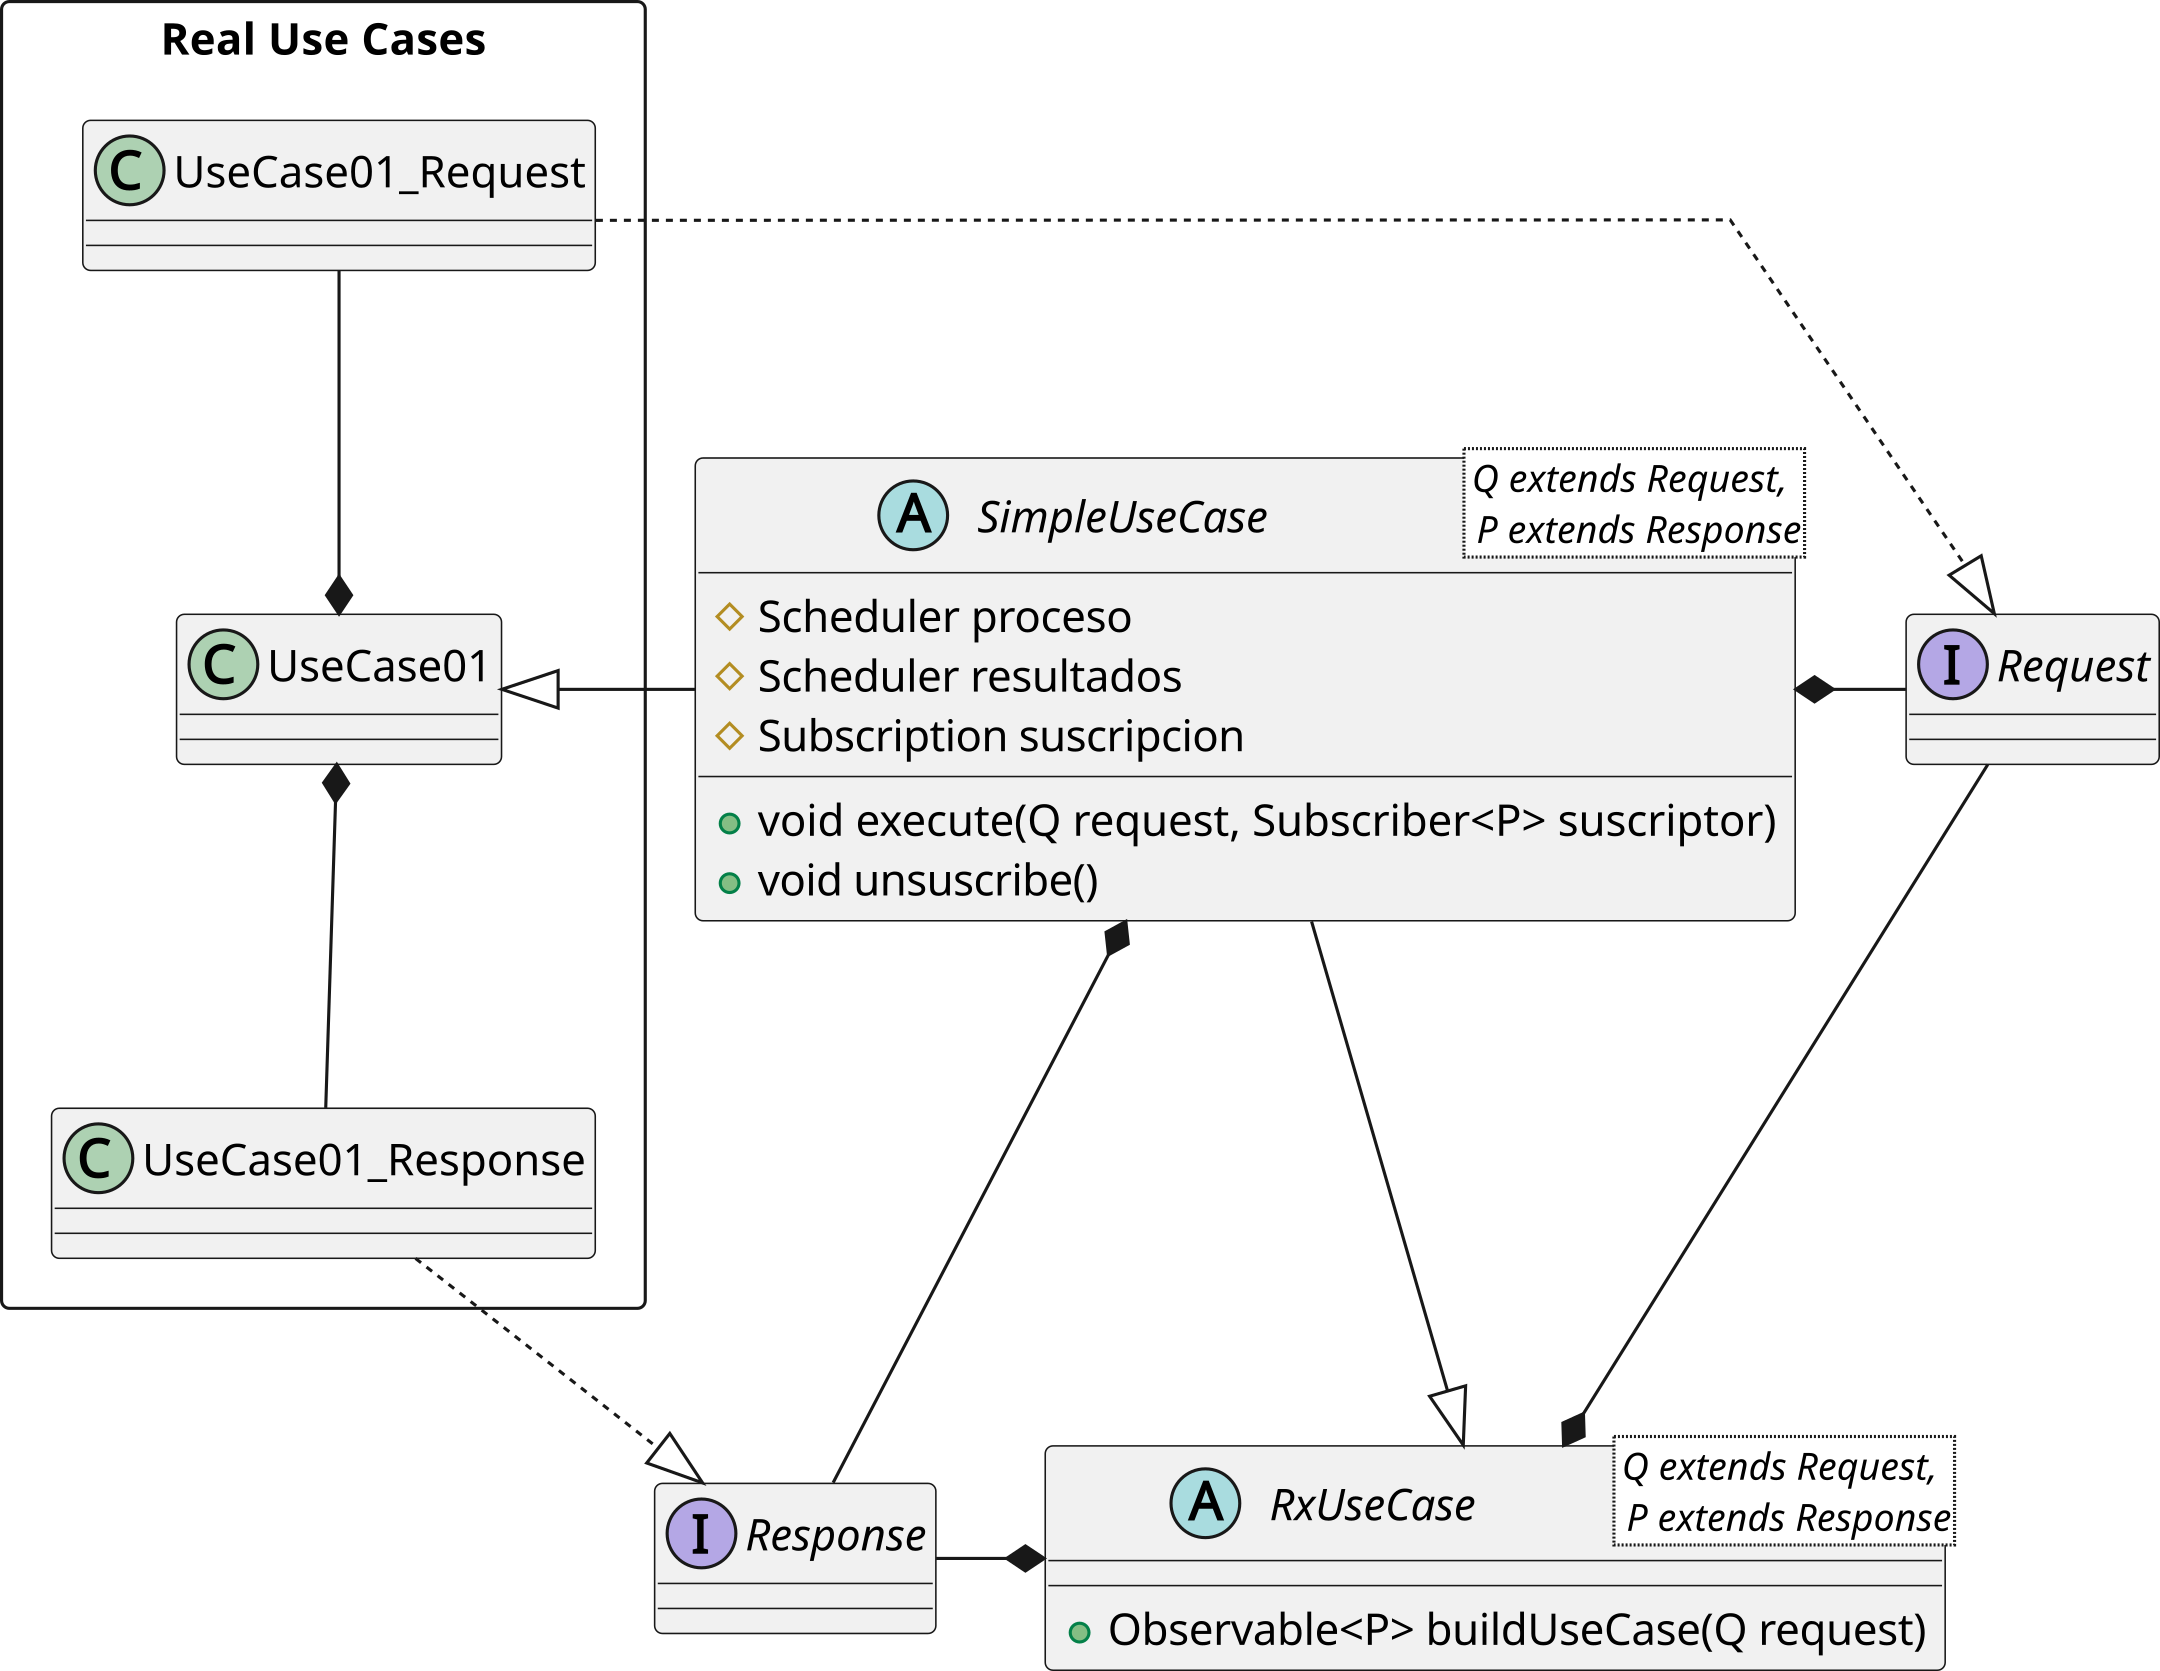
\includegraphics[width=0.8\textwidth]{Figures/iter1/CLASS_use_cases.png}
	\rule{35em}{1pt}
	\caption[Class Diagram]{Diagrama de clases de la implementación de un caso de uso.}
	\label{fig:class_usecases}
\end{figure}

\subsection{Schedulers}
En el contexto de la programación reactiva, en particular RxJava, un scheduler (planificador) es un objeto que abstrae el concepto de hilos de ejecución, controla cuándo y en qué hilo se ejecutarán las operaciones de un flujo reactivo. Es decir, proveen las instancias de hilos a las que se les asignará las tareas de los operadores en una cadena reactiva. Existen diversos Schedulers implementados por la librería, a saber:

\texttt{Schedulers.io()}\\
Optimizado para operaciones de entrada/salida (I/O), bloqueantes por definición, como llamadas de red, lectura/escritura de archivos, acceso a bases de datos, etc.
Usa un grupo de hilos que se expanden según sea necesario para acomodar la carga de trabajo I/O, y reutiliza los hilos cuando están disponibles.

\texttt{Schedulers.computation()}\\
Adecuado para operaciones computacionales que son intensivas en utilización del CPU, como cálculos matemáticos complejos.
Usa un número fijo de hilos basado en el número de núcleos del procesador, ya que tener más hilos que núcleos no mejorará el rendimiento para este tipo de tareas.

\texttt{Schedulers.newThread()}\\
Crea un nuevo hilo para cada unidad de trabajo.
No reutiliza hilos, lo que puede llevar a un consumo elevado de recursos si se usa de manera indiscriminada.

\texttt{Schedulers.single()}\\
Ejecuta todas las tareas en un solo hilo.
Útil para operaciones secuenciales donde se necesita garantizar que las tareas se ejecuten en orden sin concurrencia.

\texttt{AndroidSchedulers.mainThread()} (específico de RxAndroid)\\
Usado para ejecutar tareas en el hilo principal (UI thread) en aplicaciones Android.
Asegura que las tareas que interactúan con la UI se ejecuten en el hilo correcto.


Entendido el propósito de emplear schedulers se hace más fácil comprender la implementación del método \texttt{execute()} para la clase \texttt{SimpleUseCase}.
Cada operación de la cadena reactiva generada con \texttt{buildUseCase()} será procesada en un hilo provisto por el planificador para tareas de entrada/salida.
Así mismo las emisiones del resultado final serán capturadas por el hilo principal de la aplicación con el propósito de permitir posibles iteraciones con 
la interfaz de usuario. 

\begin{lstlisting}[caption={Método execute SimpleUseCase}, label={code:exec_usecase}, language=java, basicstyle=\ttfamily \footnotesize, numbers=left, stepnumber=1, showstringspaces=false, float]
public void execute(Q requestValues, Subscriber<P> subscriber) {
	unsubscribe();
	mSubscription = buildUseCase(requestValues)
		.subscribeOn(this.mSubscribeOn)
		.observeOn(this.mObserveOn)
		.subscribe(subscriber);
}
\end{lstlisting}

Este modo de operación multithread se especifica en las lineas 5 y 6 del código implementado para el método \texttt{excecute()} ~\ref{code:exec_usecase}
al llamar al método \texttt{subscribeOn()} se establece que todas las operaciones de la cadena reactiva se realizaran en un hilo provisto por el scheduler de E/S mientras que al llamar al método \texttt{observeOn()} como ultima operación de la cadena se fija el hilo principal de la aplicación como capturador de las emisiones del flujo de datos.

\section{Casos de Uso Implementados}
Para la presente iteración se implementaron los siguientes casos de uso.
\begin{enumerate}
	\item Buscar Módulos disponibles
	\item Solicitar Acceso
	\item Accionar Módulo
	\item Obtener datos de módulo
	\item Resetear a valores de fábrica
	\item Ingresar Credenciales WiFi
	\item Cambiar Alias	
\end{enumerate}

A continuación se documentaran aquellos que presentan los escenarios más interesantes.

\subsection{Solicitar acceso a Módulo}
Un nuevo usuario instala la aplicación cliente en su teléfono android.
Después de registrar su número telefónico, busca los módulos disponibles en la red local.
Encuentra uno y procede a solicitar acceso para que algún administrador lo autorice.
Esta operación puede utilizar hasta dos RPCs en su ejecución y puede fallar en 5 escenarios:
\begin{itemize}
	\item Error de comunicación con el módulo
	\item El módulo tuvo un error al intentar registrar al usuario
	\item Se alcanzó el máximo de usuarios admitidos por el módulo
	\item Improbable caso donde un administrador autoriza y elimina de inmediato al solicitante.
\end{itemize}
Para los escenarios 1 y 3 se permite la posibilidad de reintentar la operación una vez.
En el diagrama de la figura ~\ref{fig:act_request} se puede observar el flujo del algoritmo implementado para este caso de uso.

\begin{figure}[htbp]
	\centering
	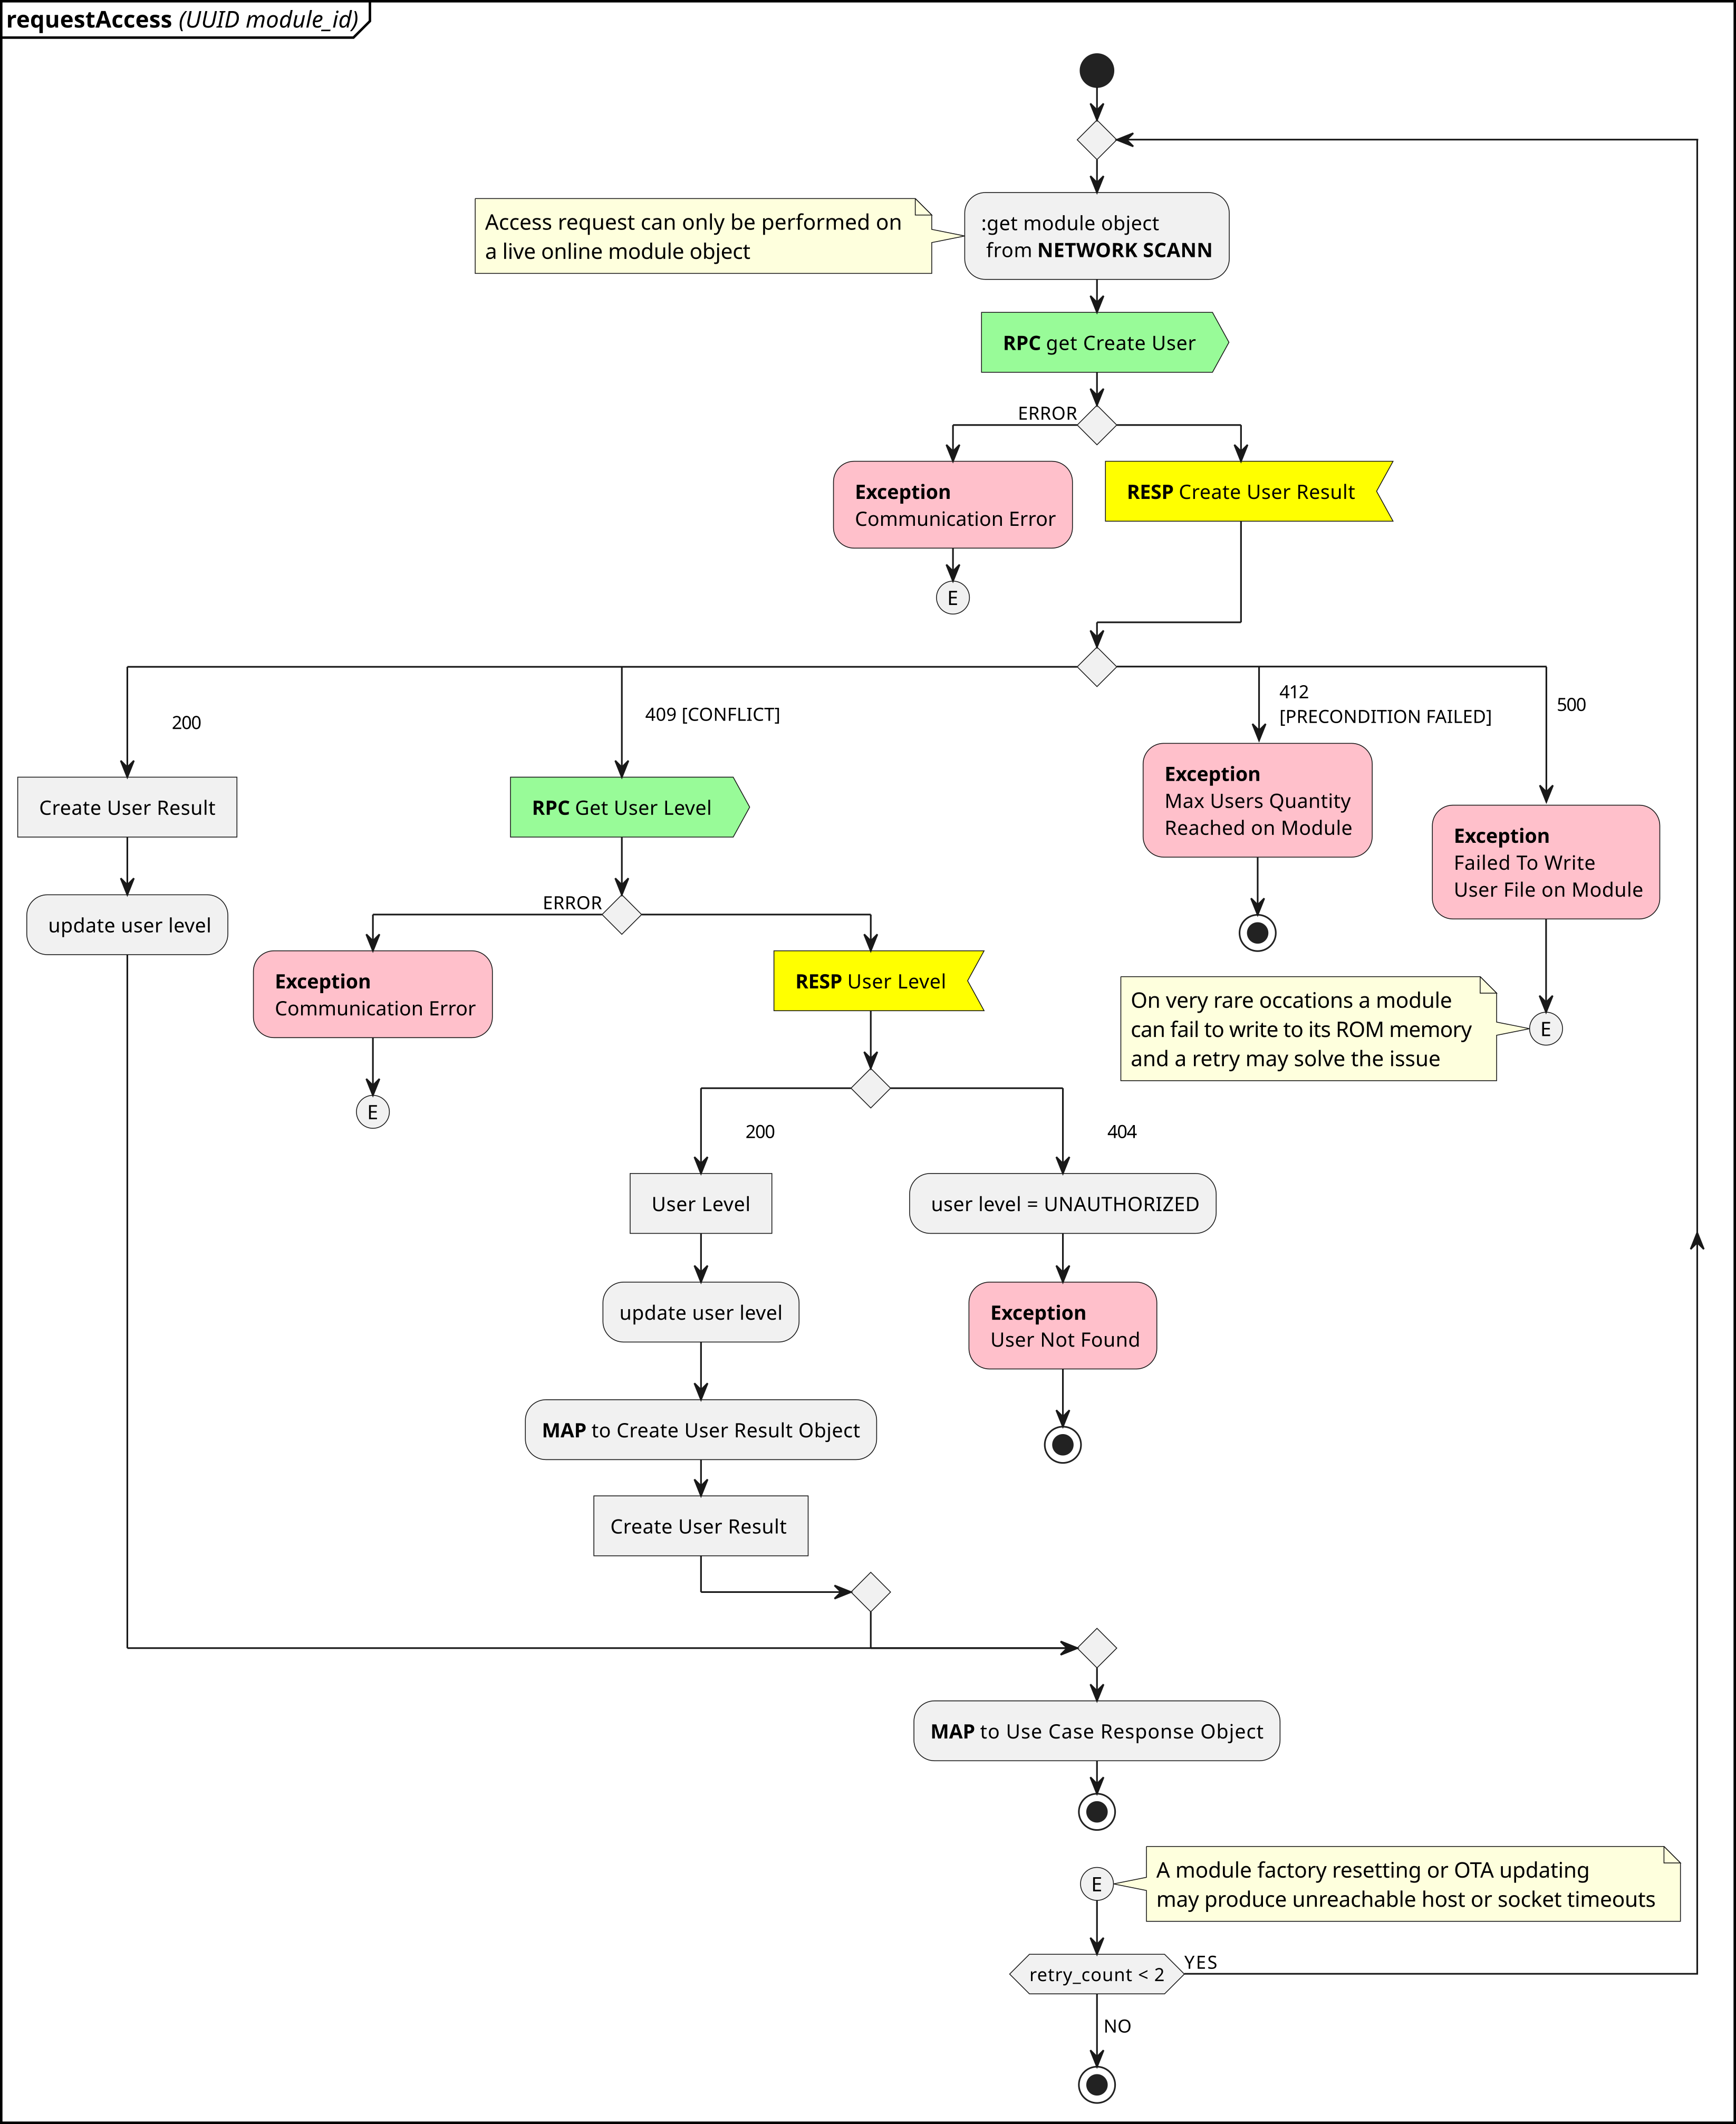
\includegraphics[width=\textwidth]{Figures/iter1/ACT_request_ink.png}
	\rule{35em}{1pt}
	\caption[Class Diagram]{Diagrama de actividades de la implementación del caso de uso: Solicitar Acceso.}
	\label{fig:act_request}
\end{figure}

\subsection{Accionar Módulo}
Un usuario abre la aplicación en su teléfono y acciona un módulo utilizando el botón deslizante.

Esta operación puede utilizar hasta dos RPCs en su ejecución y puede fallar en 3 escenarios:

\begin{enumerate}
	\item Error de comunicación con el módulo.
	\item El usuario que intenta accionar el módulo no existe.
	\item El usuario ha cambiado de nivel.
\end{enumerate}

Para los escenarios 1 y 3 se admite la posibilidad de reintentar la operación una vez.
En el diagrama de la figura ~\ref{fig:act_trigger} se puede observar el flujo del algoritmo implementado para este caso de uso.

\begin{figure}[htbp]
	\centering
	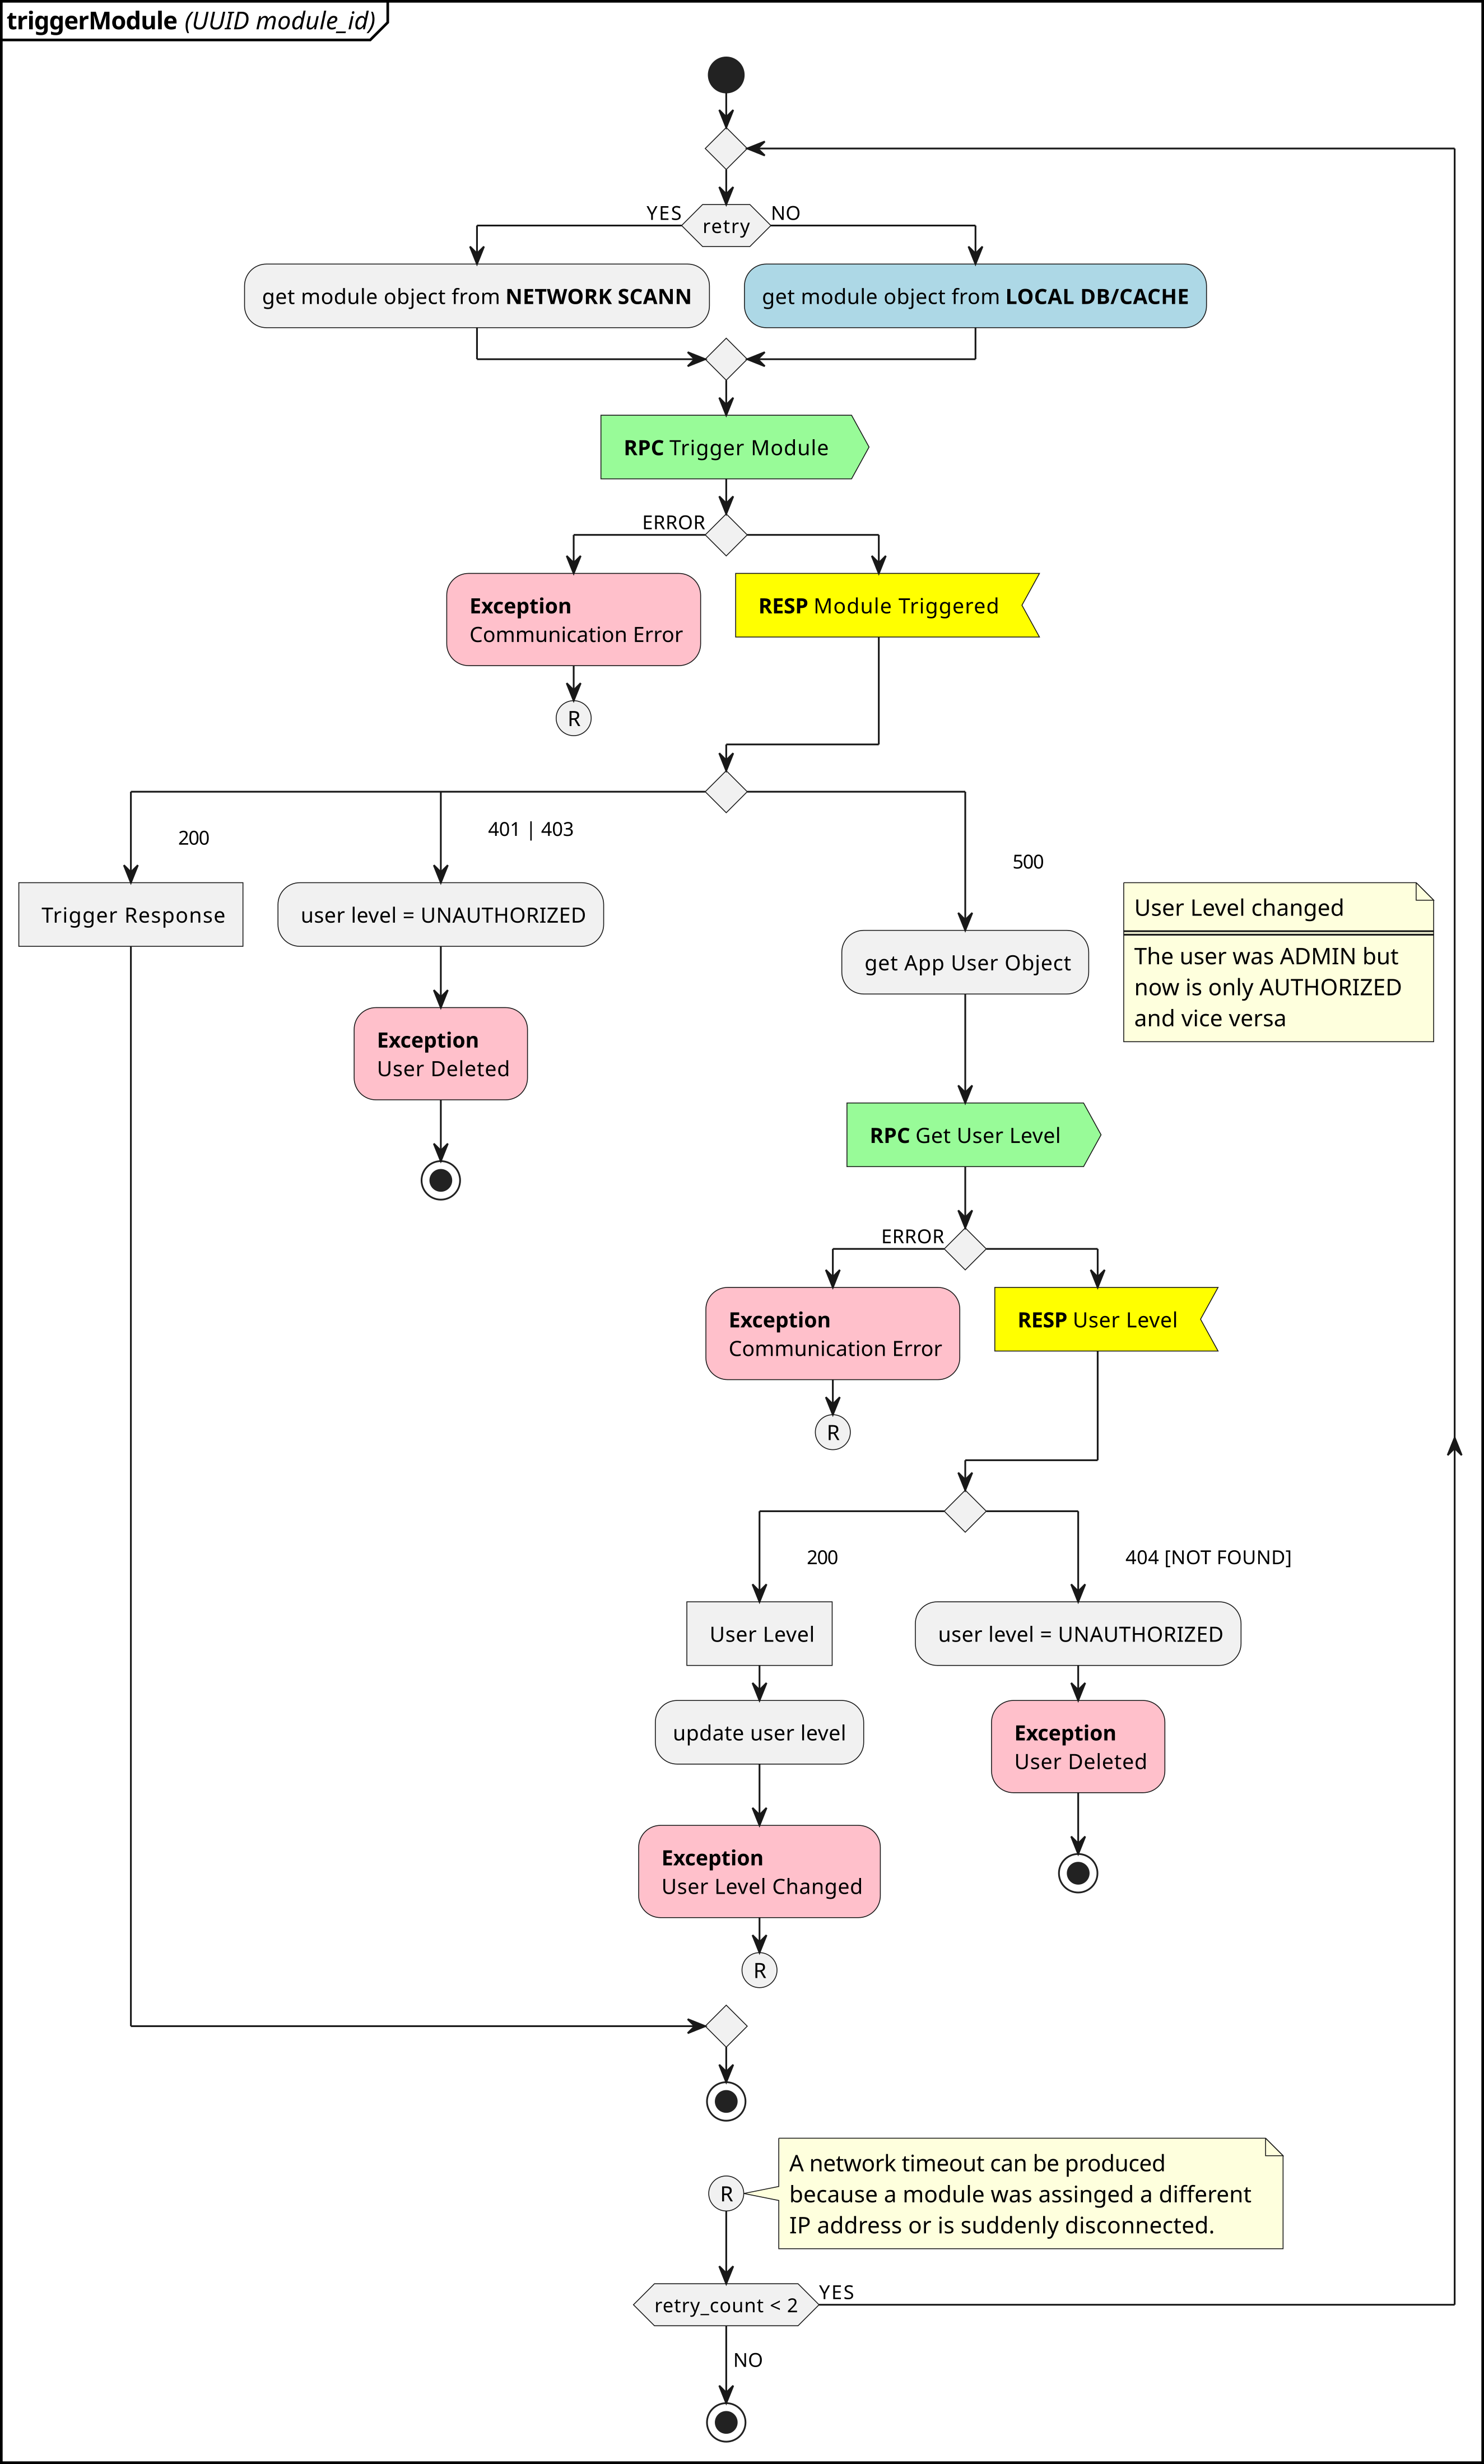
\includegraphics[width=0.8\textwidth]{Figures/iter1/ACT_trigger_module.png}
	\rule{35em}{1pt}
	\caption[Class Diagram]{Diagrama de actividades de la implementación del caso de uso: Accionar Módulo.}
	\label{fig:act_trigger}
\end{figure}

\subsection{Obtener datos del Módulo}
Un usuario toca el botón con forma de engranaje circular para acceder a las configuraciones de un módulo en particular.
Se distinguen los dos escenarios correspondientes a los modos de funcionamiento: la configuración inicial y la operación regular, descritos en la sección ~\ref{section:interfaces}.
Con el objetivo de obtener los parámetros actualizados del módulo se realizan varias operaciones en background para asegurar la consistencia de los datos y construir la UI adecuada para tal caso.

Esta operativa puede utilizar hasta tres RPCs en su ejecución y puede fallar en seis escenarios con cuatro tipos de error:

\begin{enumerate}
	\item Aplicación no conectada a módulo en configuración inicial.
	\item Error de comunicación con el módulo.
	\item El Usuario que realiza la consulta fue eliminado.
	\item Formato de consulta RPC erróneo.
\end{enumerate}

En el diagrama de la figura ~\ref{fig:act_get_umod_data} se puede observar el flujo del algoritmo implementado para este caso de uso.

\begin{figure}[htbp]
	\centering
	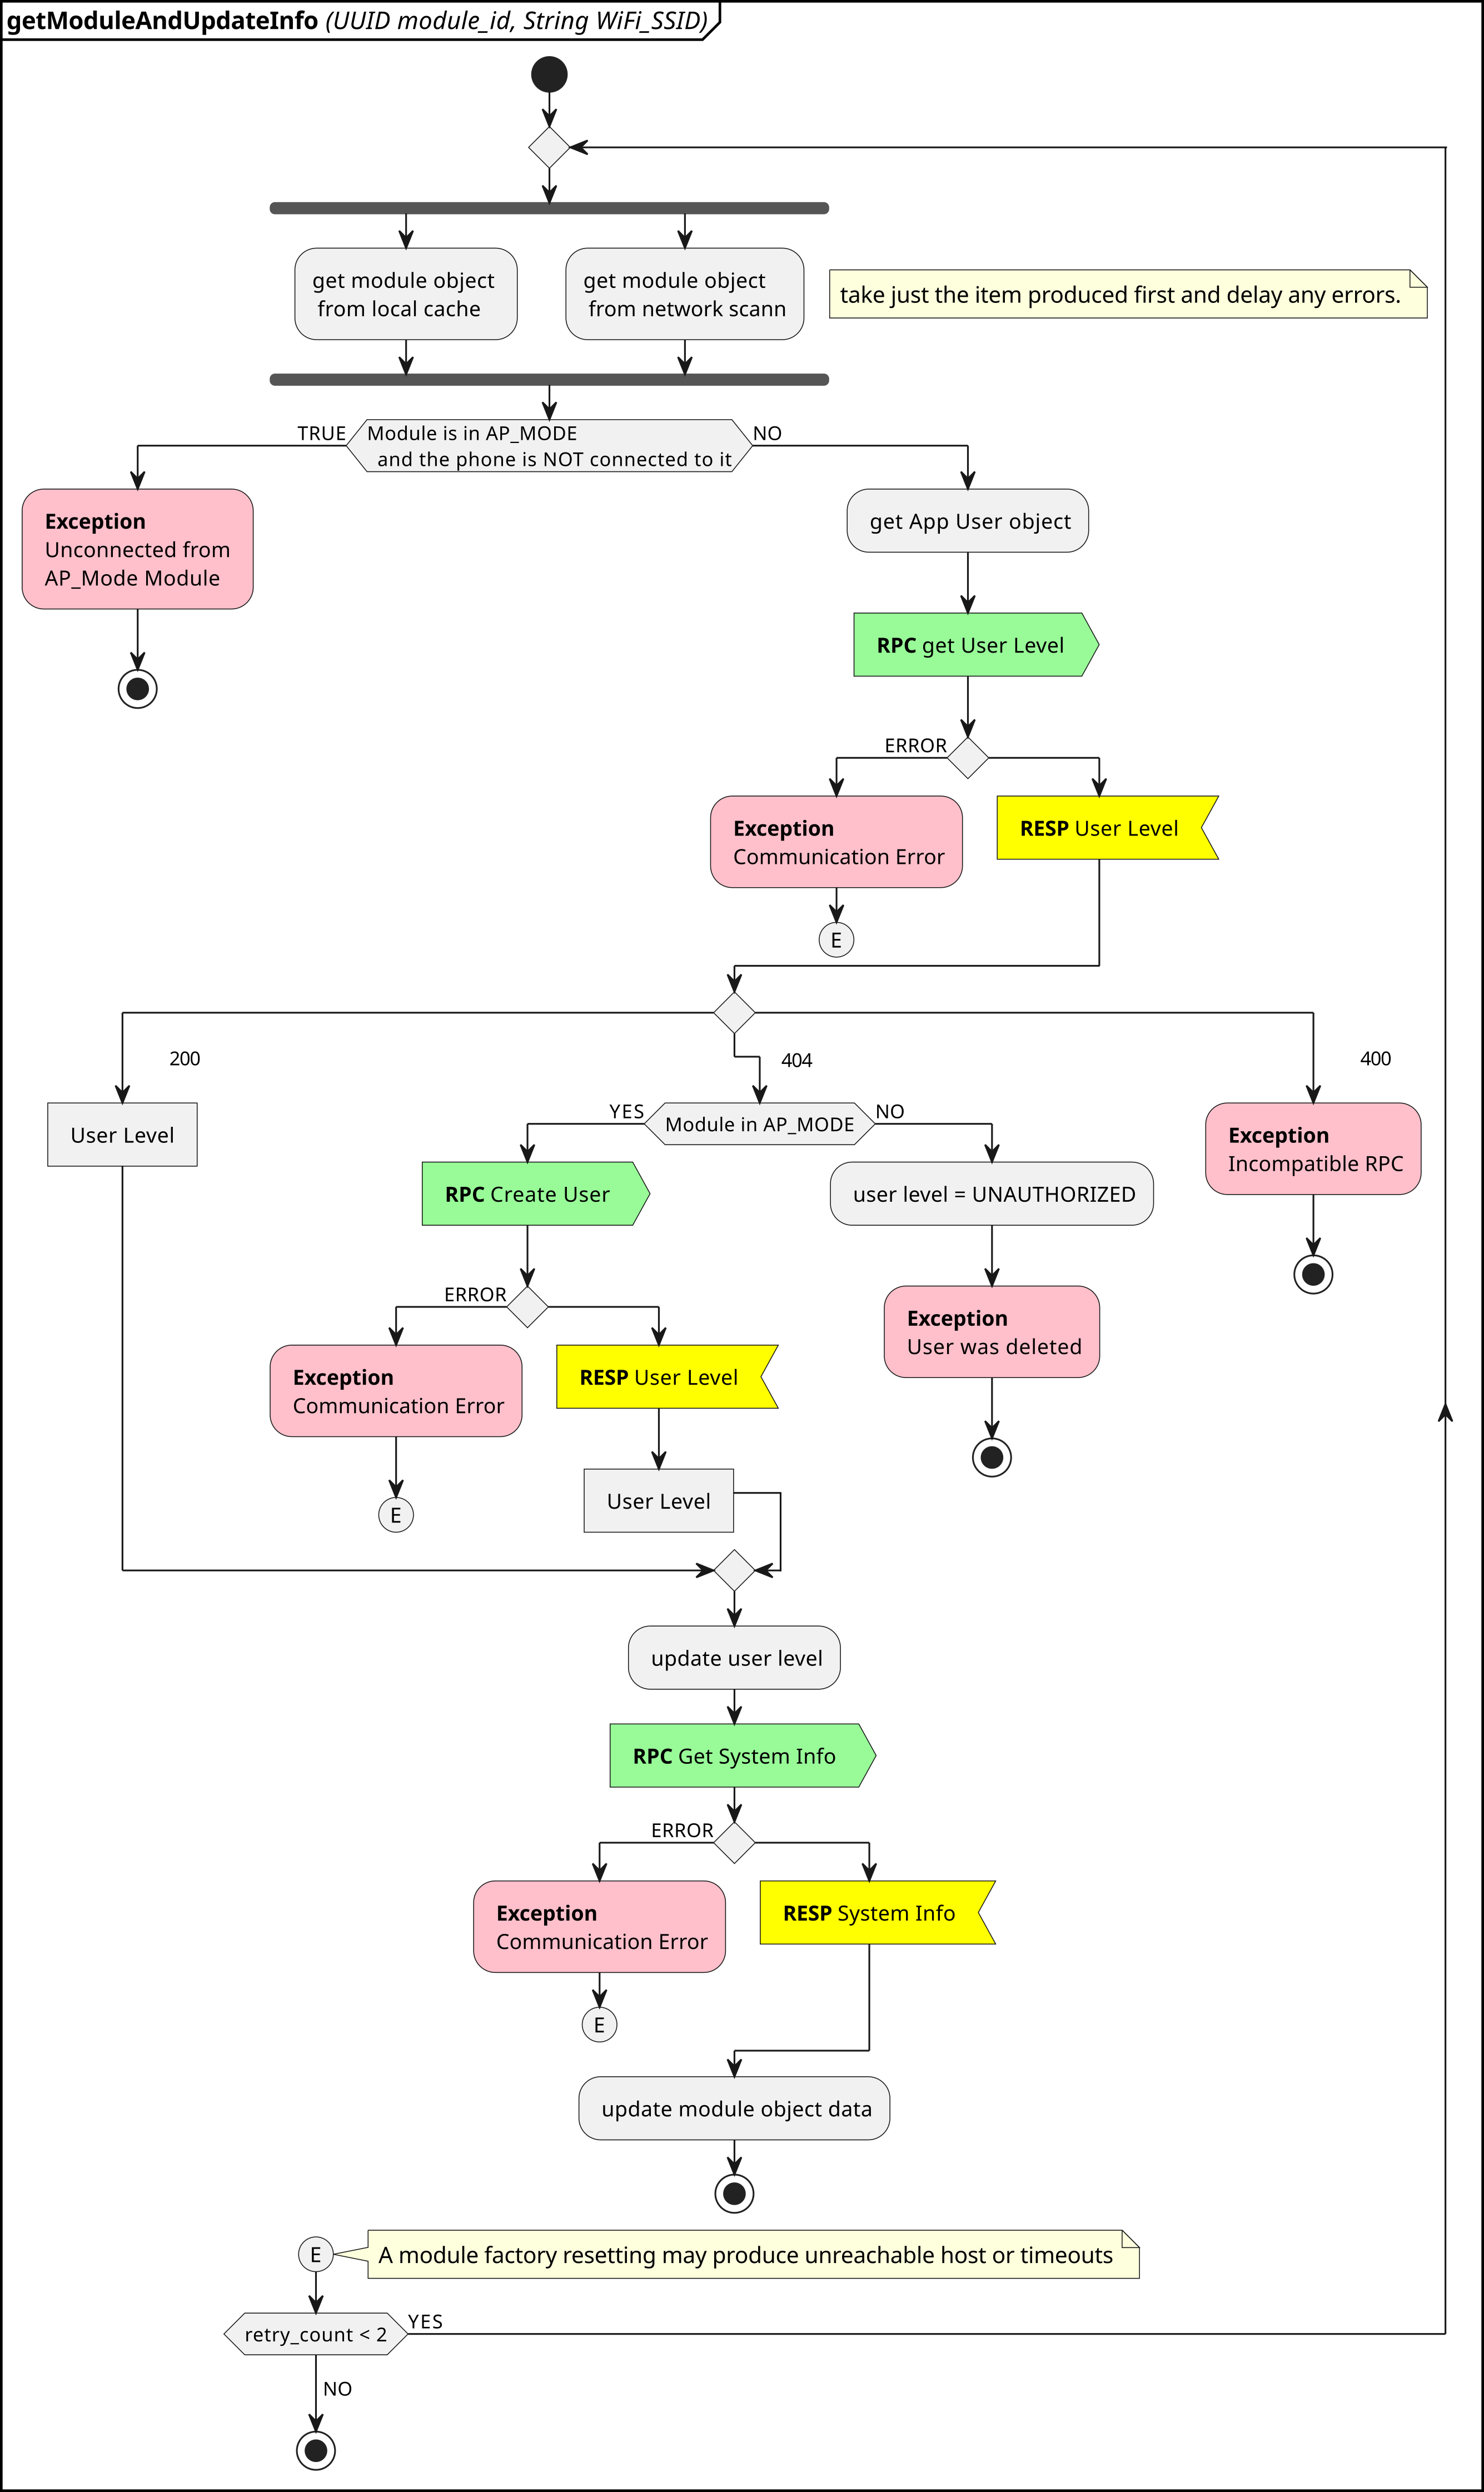
\includegraphics[width=0.8\textwidth]{Figures/iter1/ACT_getModuleAndUpdateInfo_ink.png}
	\rule{35em}{1pt}
	\caption[Class Diagram]{Diagrama de actividades de la implementación del caso de uso: Accionar Módulo.}
	\label{fig:act_get_umod_data}
\end{figure}

\section{Repositorio Objetos Módulo}
\subsection{Objeto Módulo: UMod}
Los módulos electrónicos se representan en el código de la aplicación como objetos de tipo UMod 
estas entidades mantendrán registro de tres atributos enumerados a saber.
\begin{enumerate}
	\item \textbf{STATE}: es un reflejo exacto de la máquina de estados implementada en el firmware del módulo.
	\item \textbf{STATUS}: hace referencia al reporte de apertura del sistema dónde está instalado el módulo.
	\item \textbf{SOURCE}: indica el origen de la última actualización de este objeto.
\end{enumerate}

\begin{figure}[htbp]
	\centering
	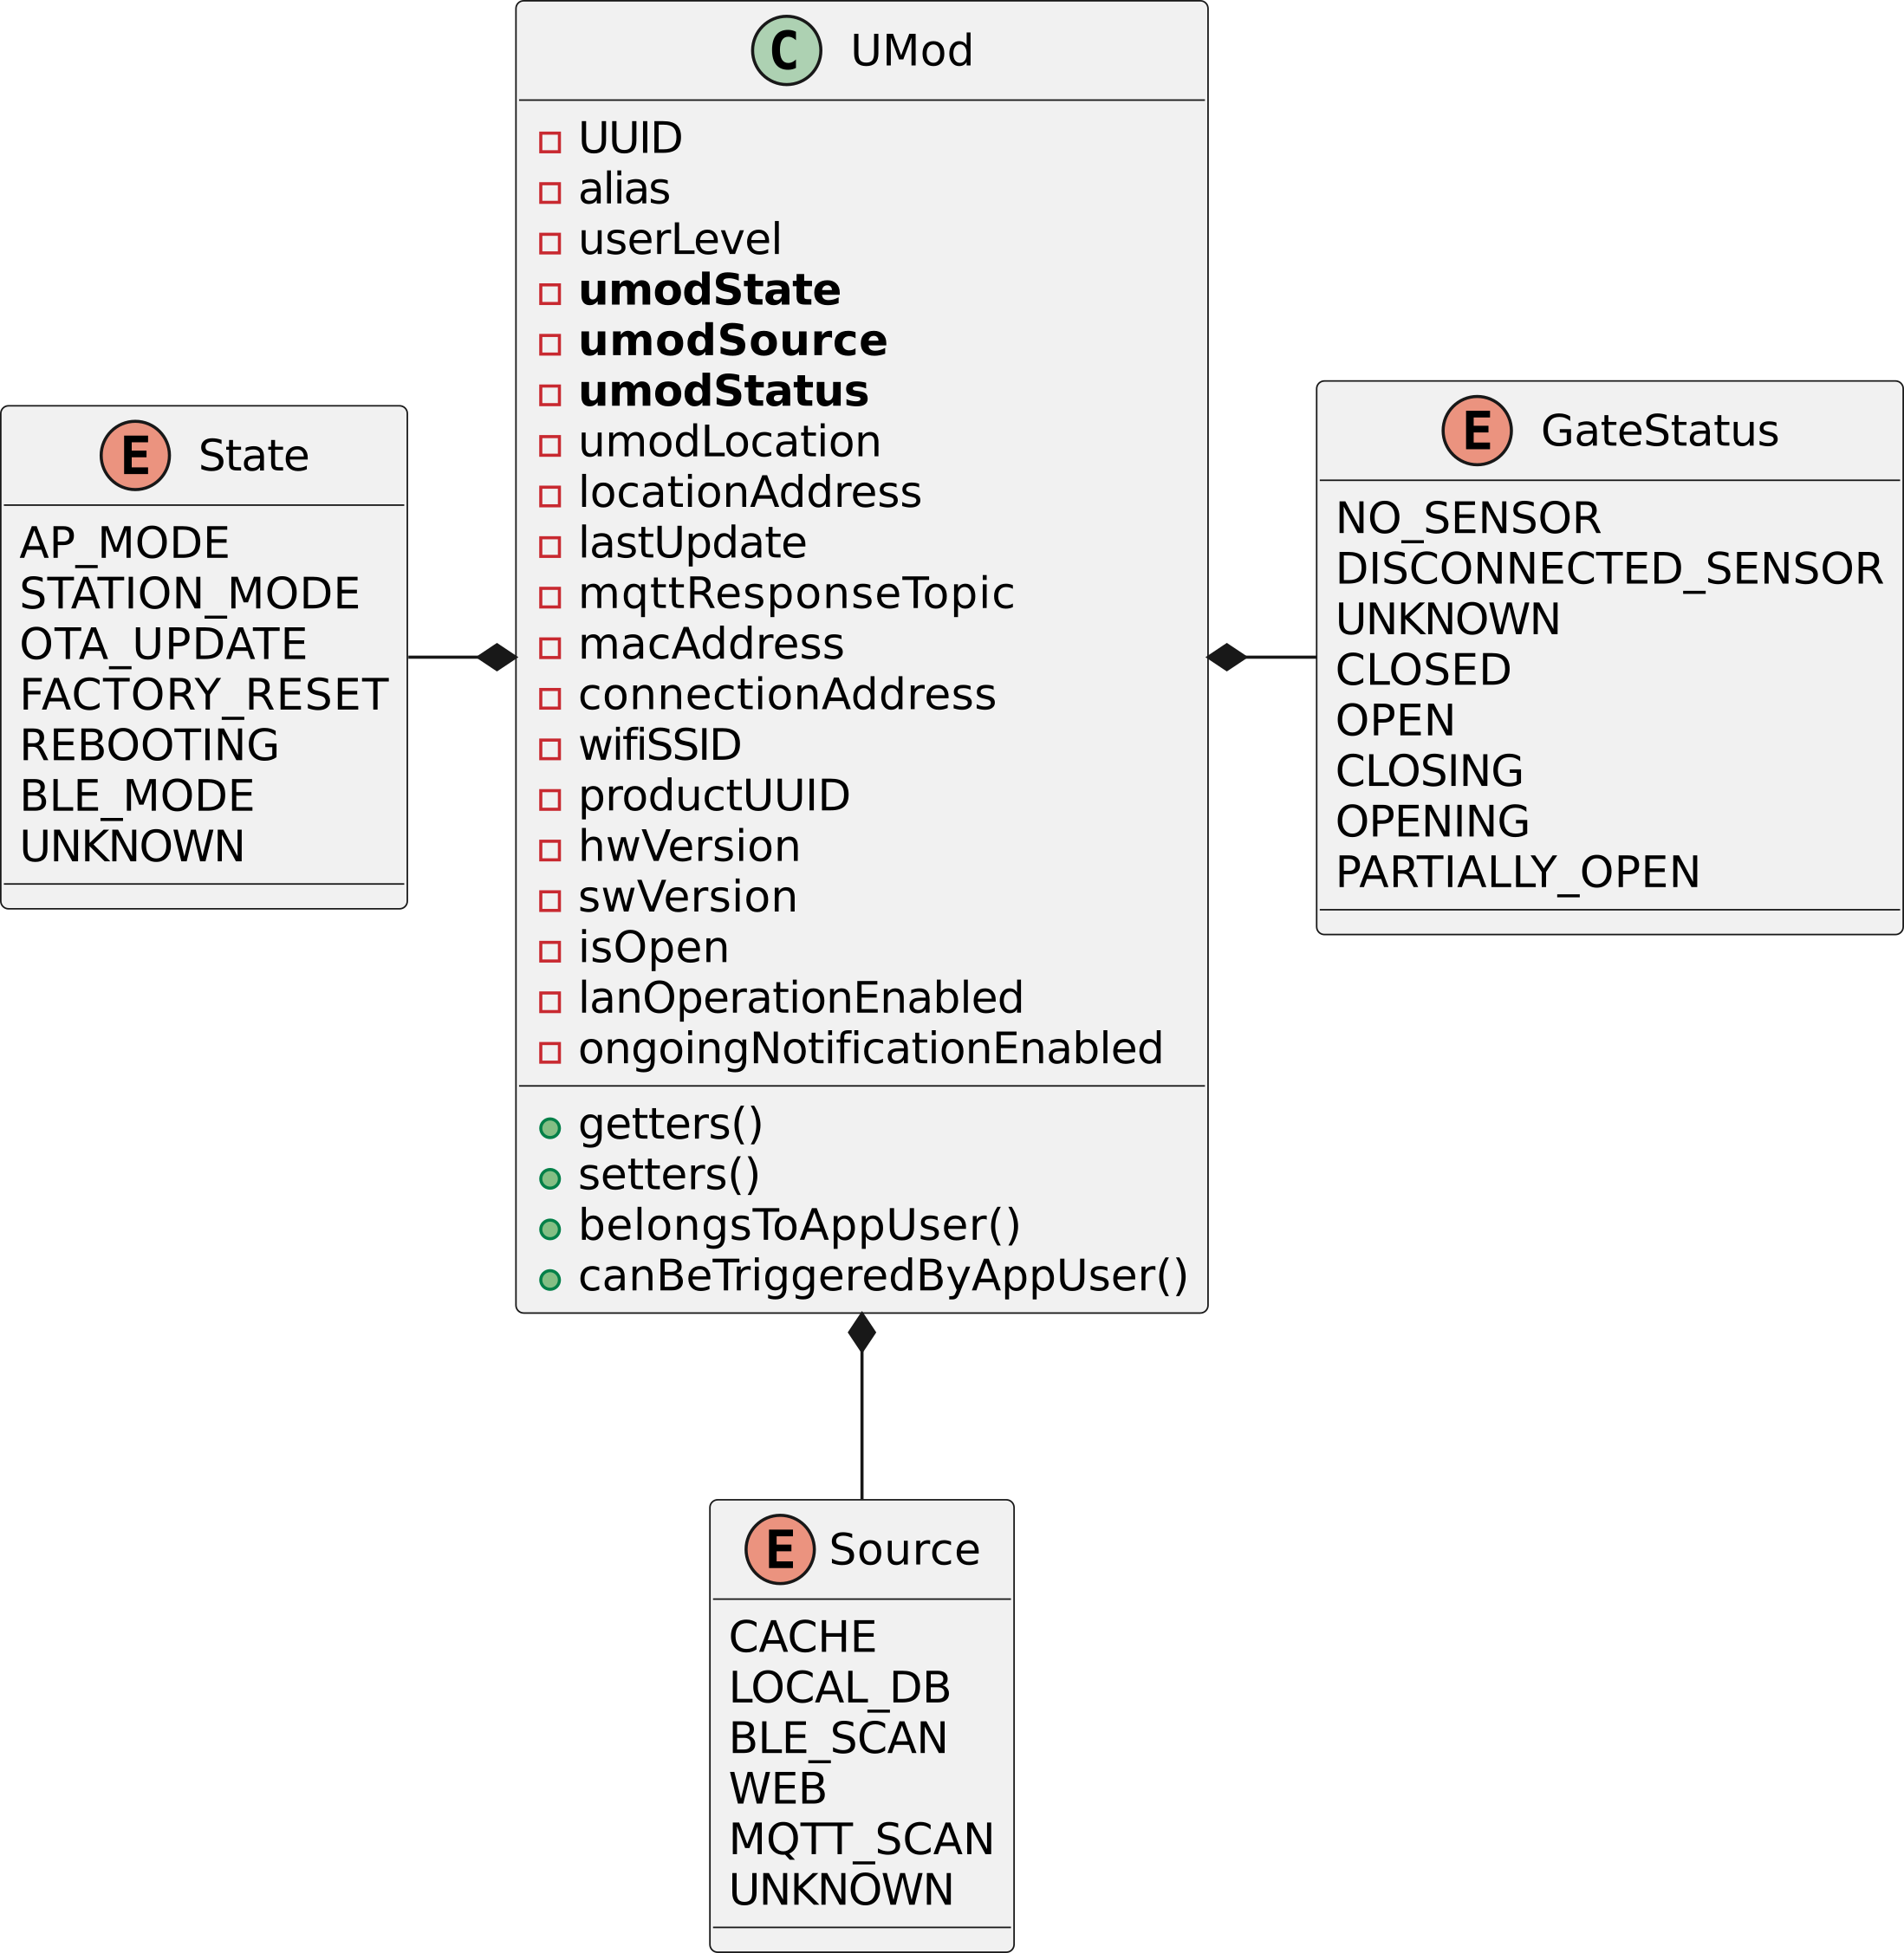
\includegraphics[width=0.7\textwidth]{Figures/iter1/CLASS_umod_ink.png}
	\rule{35em}{1pt}
	\caption[Class Diagram]{Diagrama de clases de la implementación del Objeto Módulo.}
	\label{fig:class_umod}
\end{figure}

Los demás atributos se muestran el la figura ~\ref{fig:class_umod} son auto-descriptivos y serán utilizados para popular la interfaz gráfica y para realizar las operaciones soportadas por la aplicación.

\subsection{Repositorio}
Las operaciones CRUD de estos objetos son responsabilidad del objeto repositorio que debería instanciarse a modo \texttt{singleton} para asegurar la consistencia de sus operaciones. Tal como fue introducido en la sección de diseño ~\ref{section:repository}, las tareas de persistencia y comunicación con los objetos módulo se implementarán utilizando el patrón de diseño \texttt{repository} con las modificaciones documentadas. Si se comparan las figuras ~\ref{fig:uml_clases_modif_repository} y ~\ref{fig:class_umods_repository} puede observarse como la implementación en el código de la aplicación respeta tal diseño. Se escribirán cada una de las operaciones soportadas como RPC en métodos individuales, en el diagrama de clases solo se muestra uno a modo ilustrativo.

\begin{figure}[htbp]
	\centering
	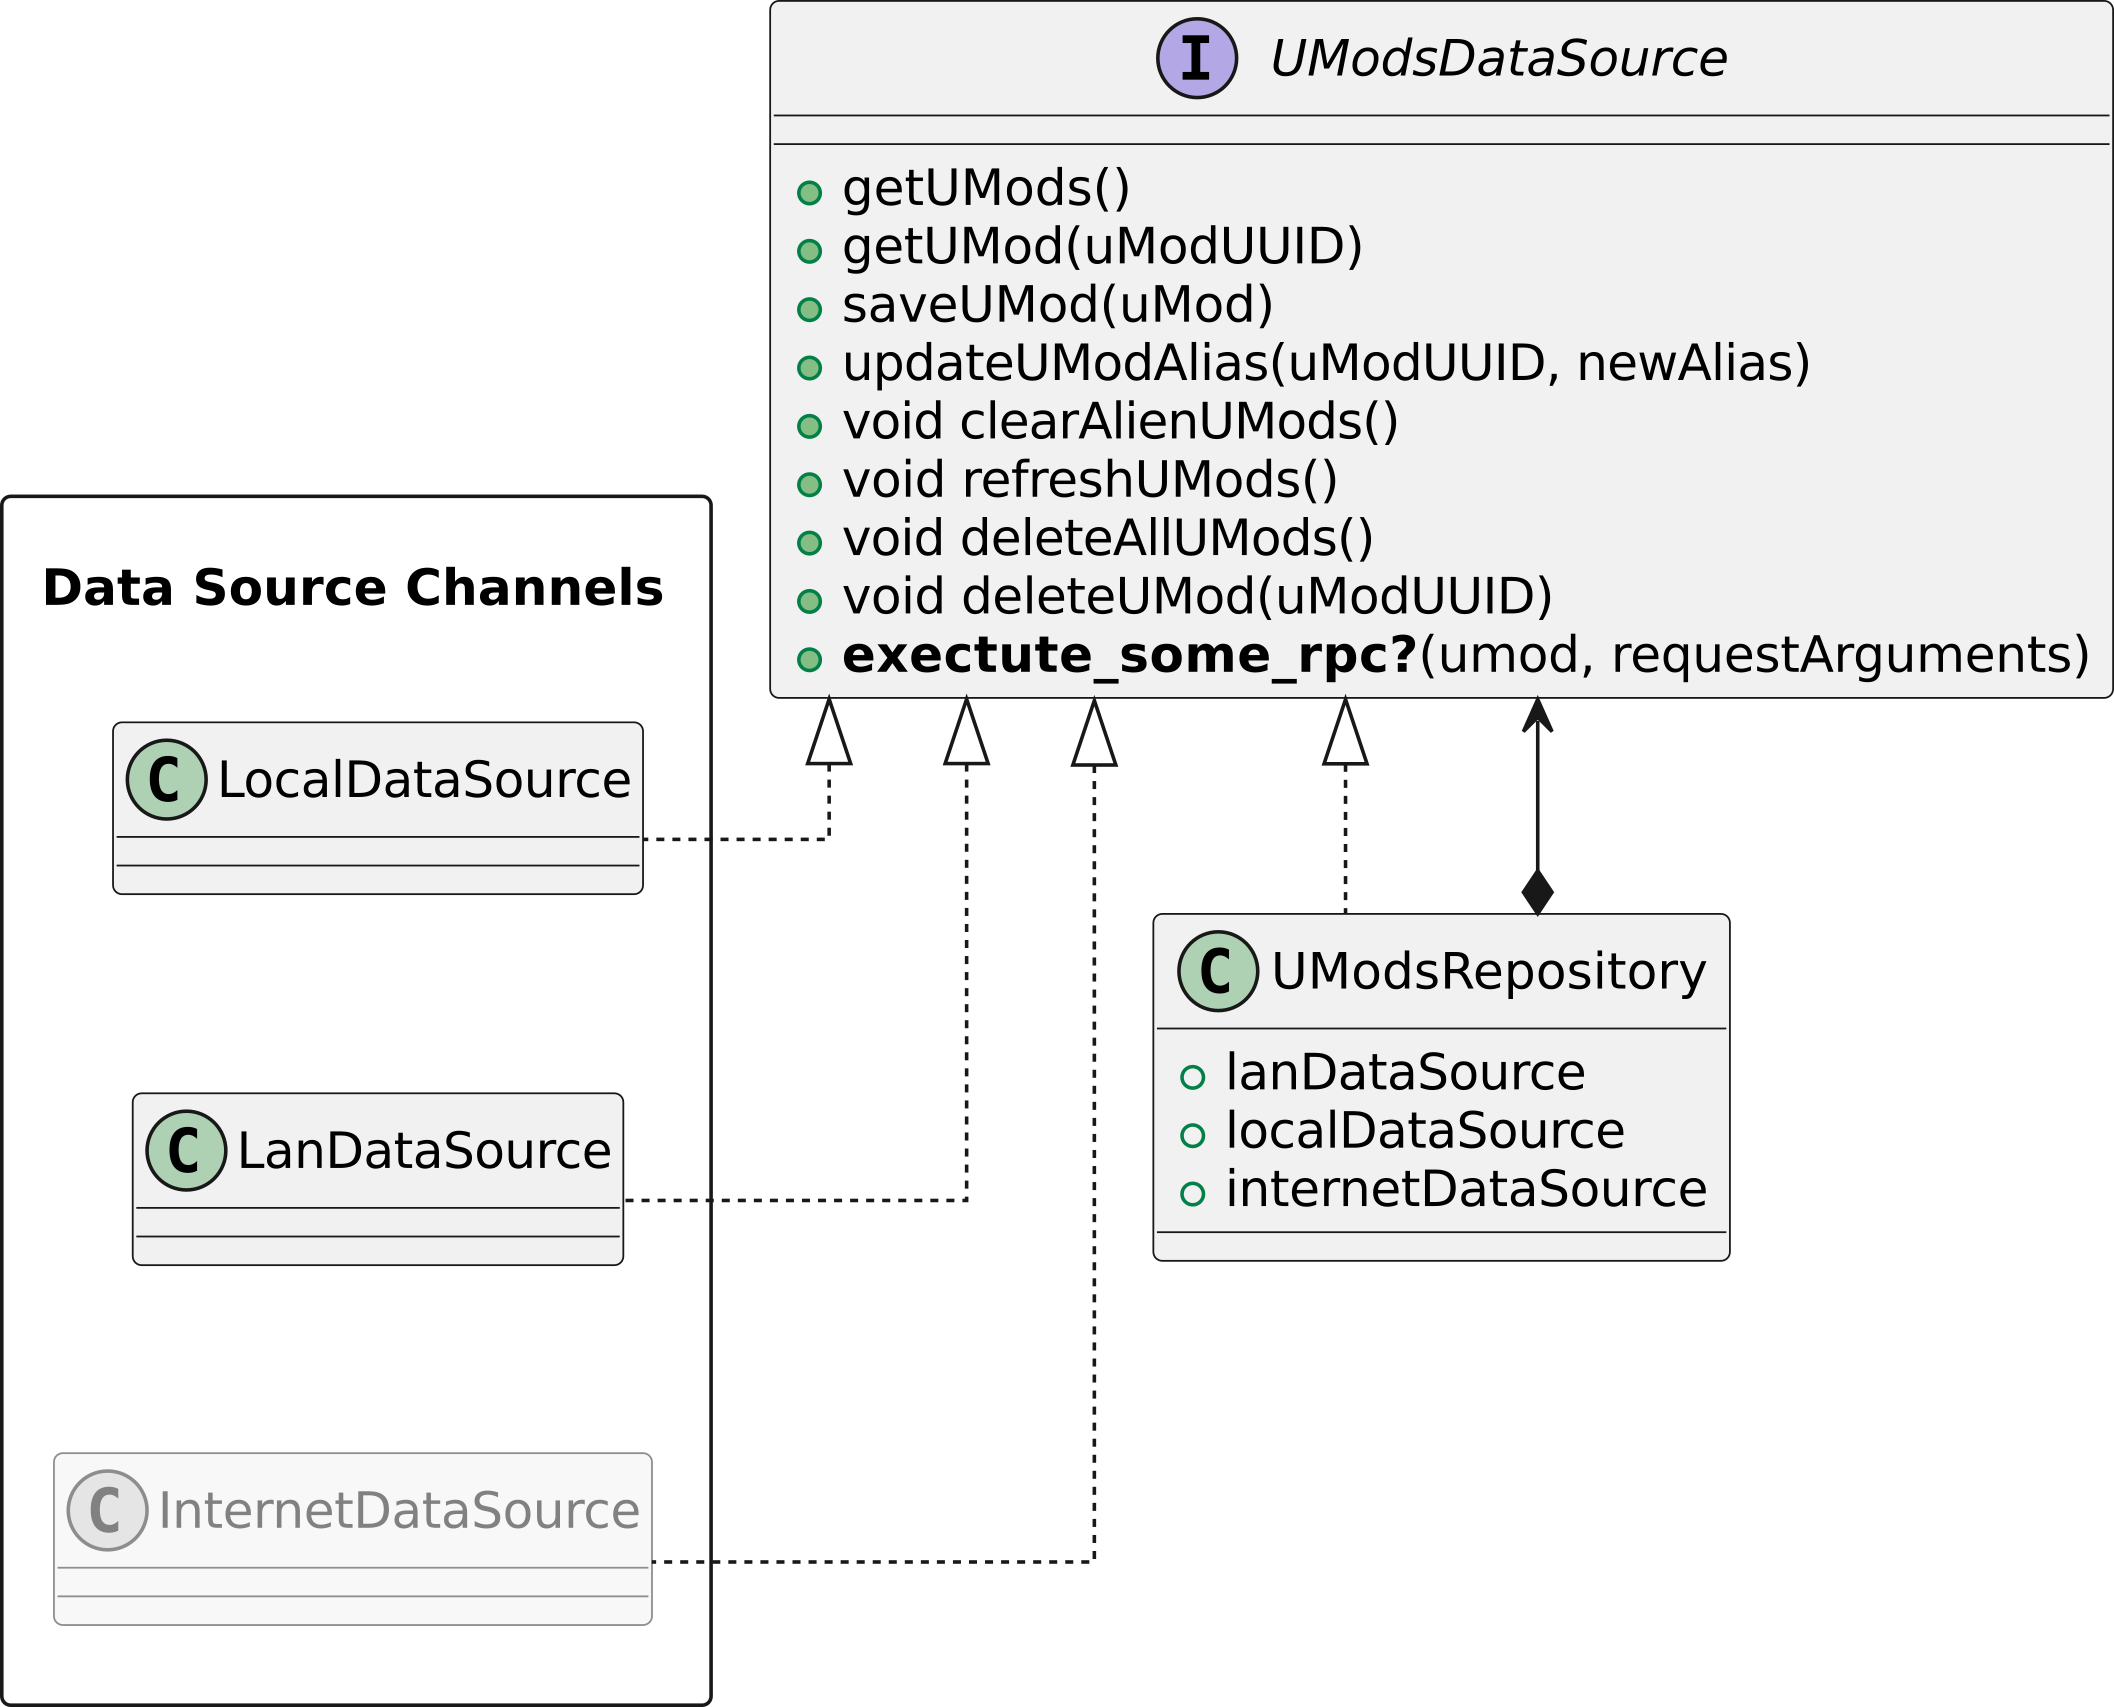
\includegraphics[width=0.7\textwidth]{Figures/iter1/CLASS_umods_repository_ink.png}
	\rule{35em}{1pt}
	\caption[Class Diagram]{Diagrama de clases de la implementación del Repositorio para los objetos módulo.}
	\label{fig:class_umods_repository}
\end{figure}

Dado que todos los canales de origen de datos para el repositorio fueron implementados como emisores reactivos se hace un uso intensivo de operadores sobre flujos reactivos. Se evidencian tanto la complejidad como la gran utilidad de el empleo de este paradigma.

\subsubsection{Canal de Persistencia Local}
Para mantener un registro local de módulos configurados y utilizados por el usuario es necesario utilizar alguna forma de persistencia local en el dispositivo. Se optó por utilizar sqlite y un wrapper reactivo para acceder a la base de datos. Los módulos configurados son almacenados en las filas de una única tabla. Como todos los canales de datos implementan la misma interfaz \texttt{UModuleDataSource} los métodos asignados a la ejecución de los RPC quedan vacíos para este canal. 

\subsubsection{Canal de Comunicación de Área Local}
Con el objetivo de poder ejecutar los protocolos remotos (RPCs) se declara un canal para comunicación HTTP.
Para ello se utilizó la librería Retrofit que provee un wrapper reactivo out-of-the-box y permite la configuración de las
solicitudes http a modo declarativo dejando oculto los pormenores del protocolo de comunicación.
Fue necesario incorporar un interceptor de solicitudes para habilitar el método de autenticación por digesto documentado en la sección ~\ref{section:digest}.
% Chapter Template

\chapter{Desarrollo: Iteración II} % Main chapter title

\label{Chapter7} % Change X to a consecutive number; for referencing this chapter elsewhere, use \ref{ChapterX}

\steveCabecera{Capítulo 7. \emph{Iteración II}} % Change X to a consecutive number; this is for the header on each page - perhaps a shortened title

%----------------------------------------------------------------------------------------
%	SECTION 1
%----------------------------------------------------------------------------------------
\section{Introducción}
En este capítulo se documentan aspectos relevantes relacionados con la codificación que se realizó en la segunda iteración de desarrollo del software.\\
Se explicaran los Casos de Uso más interesantes de los contemplados para esta iteración.
Se comentará sobre el repositorio de locaciones con el que se obtendrá la información de ubicación del teléfono.
Finalmente se introducirá la metodología, conceptos y herramientas utilizadas para realizar las pruebas unitarias y funcionales.

\section{Casos de Uso Implementados}
Para la presente iteración se implementaron los siguientes casos de uso.
\begin{enumerate}
	\item Calibrar Módulo
	\item Borrar Módulos Inaccesibles
	\item Resetear Calibración
	\item Actualizar Geolocalización
	\item Eliminar Usuario
	\item Crear Usuario
\end{enumerate}

A continuación se documentaran aquellos que presentan los escenarios más interesantes.

\subsection{Resetear Calibración}
Un usuario de nivel administrador ingresa a la pantalla de configuración de un módulo y presiona el botón 
para reiniciar la calibración de dicho módulo.
Esta operación ejecuta el RPC para modificar el atributo GATE-STATUS almacenado en el módulo y le asigna el valor UNKNOWN
de forma tal que la próxima vez que algún usuario accione dicho módulo se activará el wizard de calibración.
Este caso de uso utiliza solo un RPC y falla en dos escenarios con dos tipos de error

\begin{itemize}
	\item Error de comunicación con el módulo
	\item El usuario fue eliminado del módulo.
\end{itemize}

En el diagrama de la figura ~\ref{fig:act_resetCalib} se puede observar el flujo del algoritmo implementado para este caso de uso.
\begin{figure}[htbp]
	\centering
	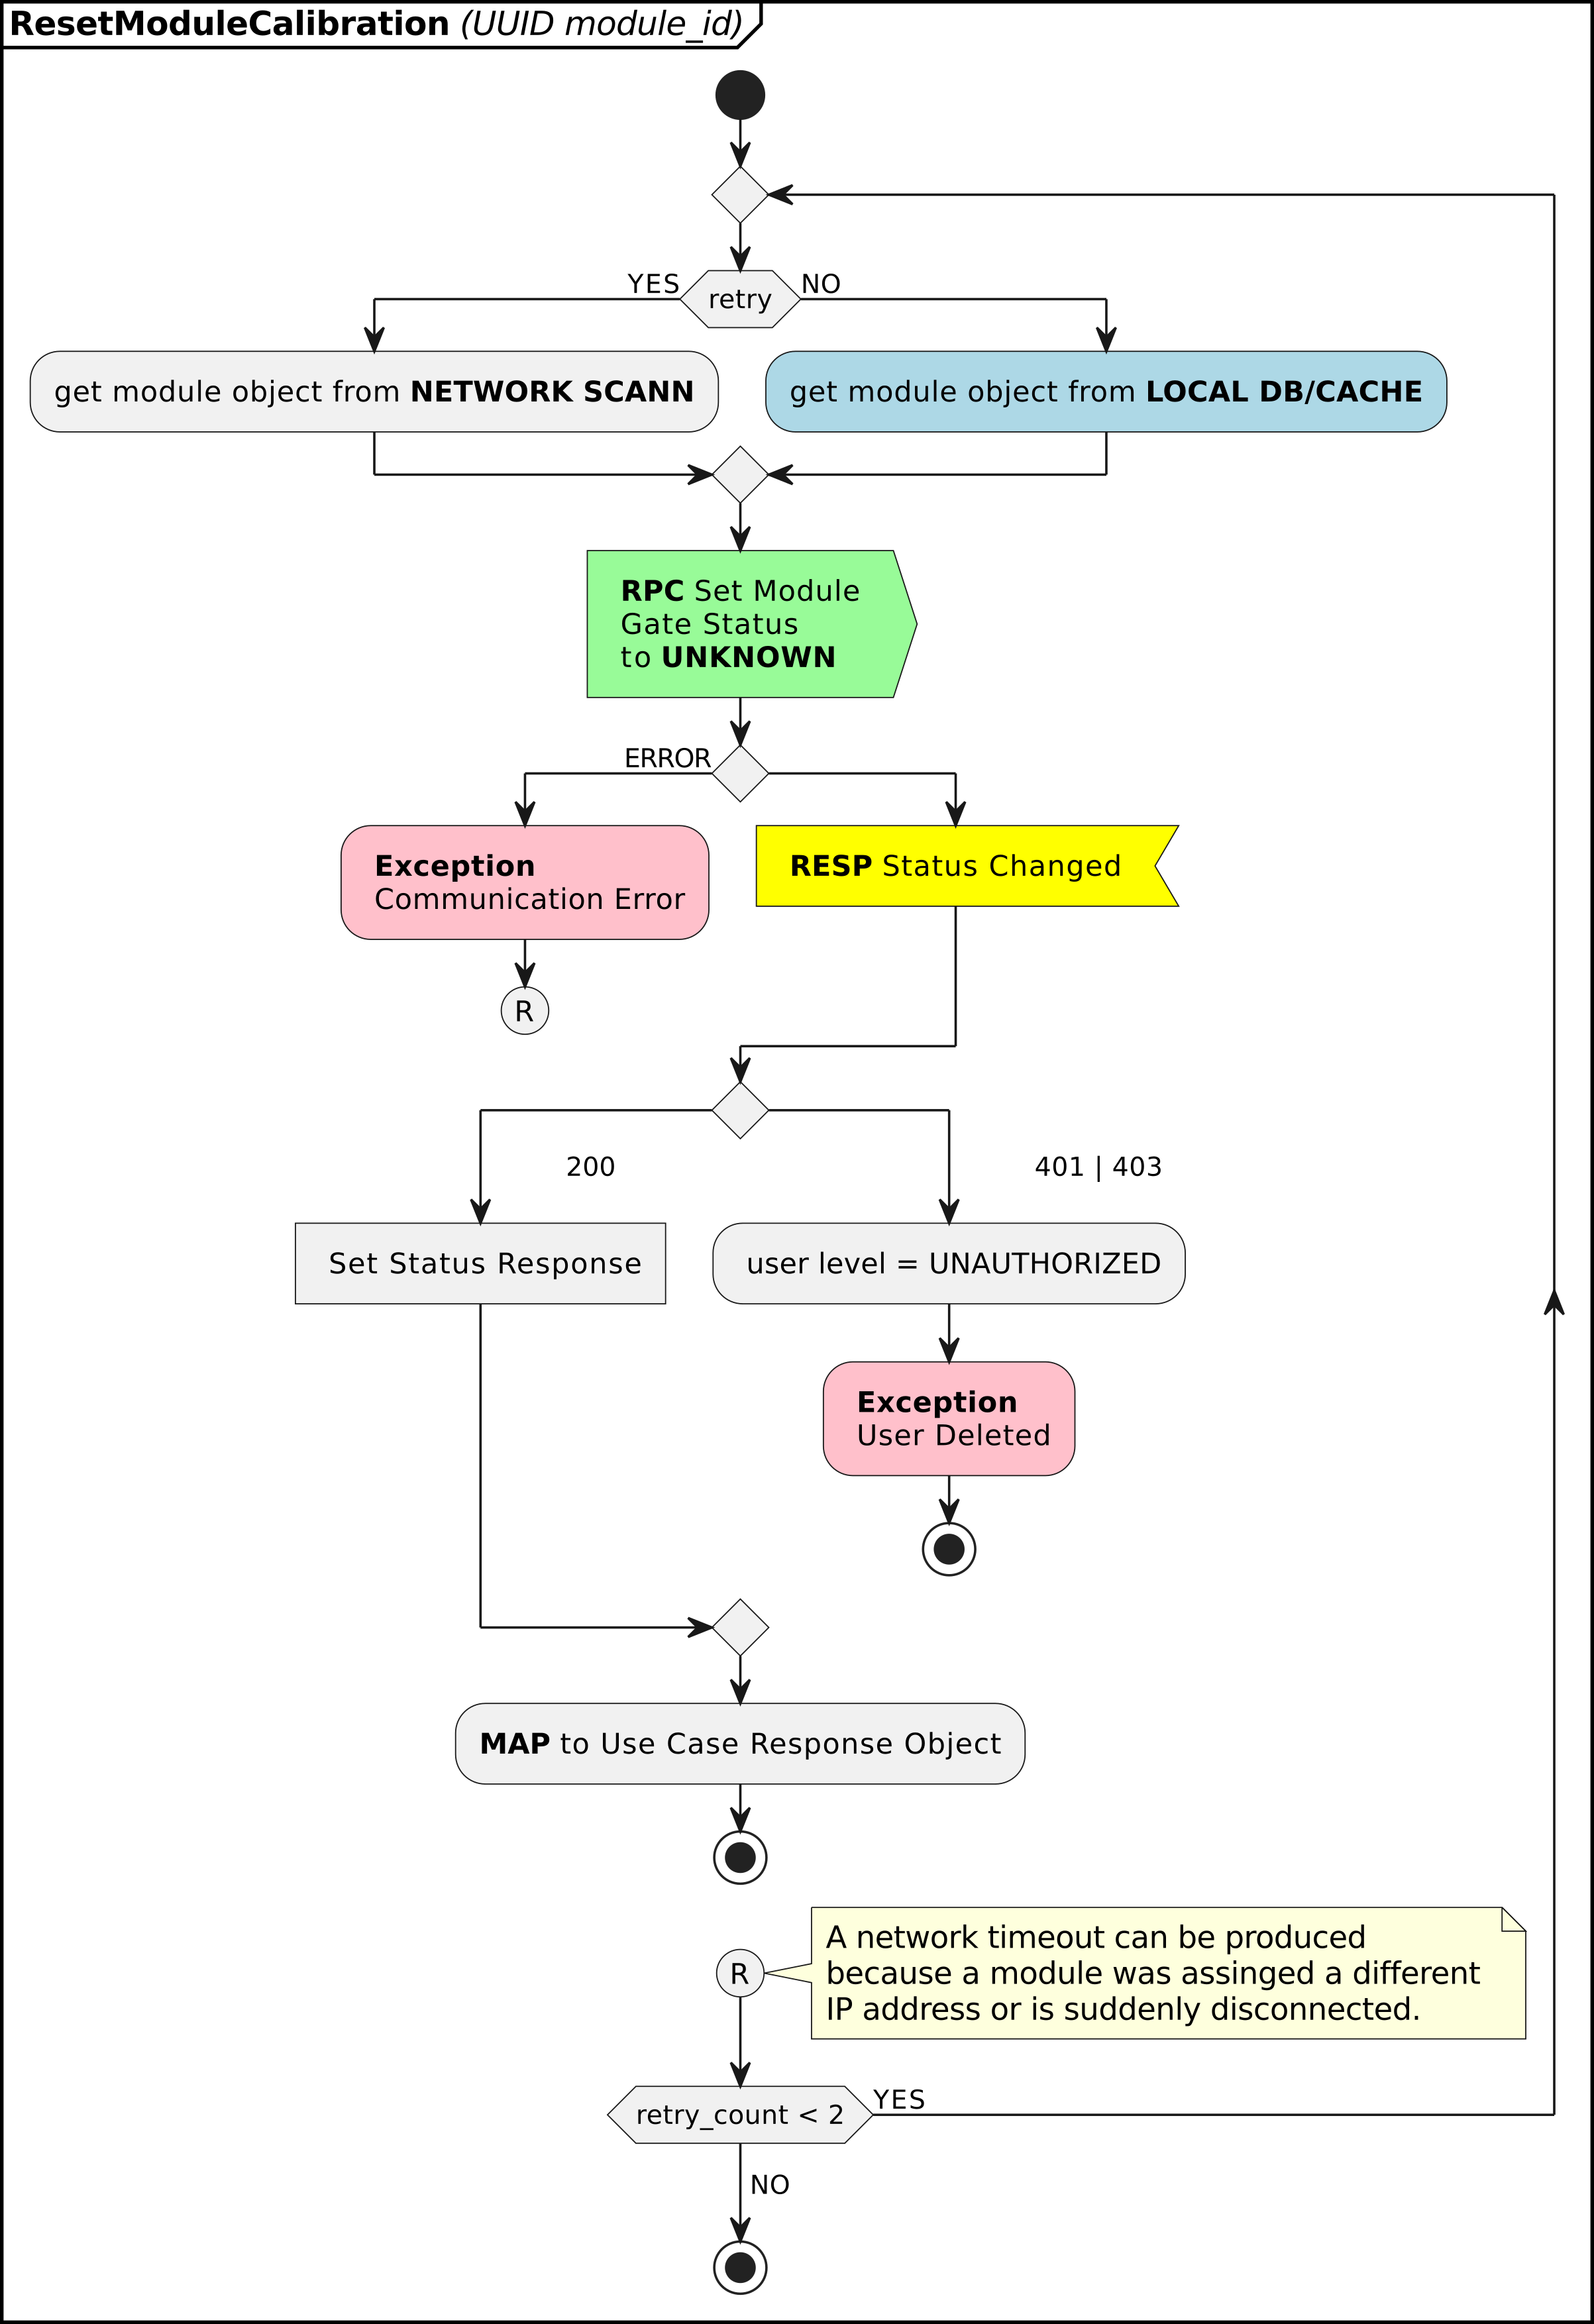
\includegraphics[width=0.8\textwidth]{Figures/iter2/ACT_resetCalib.png}
	\rule{35em}{1pt}
	\caption[Class Diagram]{Diagrama de actividades de la implementación del caso de uso: Resetear Calibración.}
	\label{fig:act_act_resetCalib}
\end{figure}

\subsection{Obtener Geolocalización}
Un usuario ingresa a la pantalla de configuración de un módulo y toca el ícono de ubicación.
Esta acción debería actualizar el texto que indica latitud, longitud y la dirección urbana que se desea asignar a dicho módulo.
Para esta operación no se ejecuta ningún RPC sino que se trata de llamadas a métodos de la librería Android-ReactiveLocation por mcharmas, que hace de interfaz reactiva con el servicio de ubicación de android.
El caso de uso puede fallar en 2 escenarios cuando los métodos no generan resultados después de realizar las consultas.
Para ambos escenarios se contempla el re-intento de hasta 3 veces ya que obtener resultados nulos es una situación frecuente.

En el diagrama de la figura ~\ref{fig:act_geoloc} se puede observar el flujo del algoritmo implementado para este caso de uso.

\begin{figure}[htbp]
	\centering
	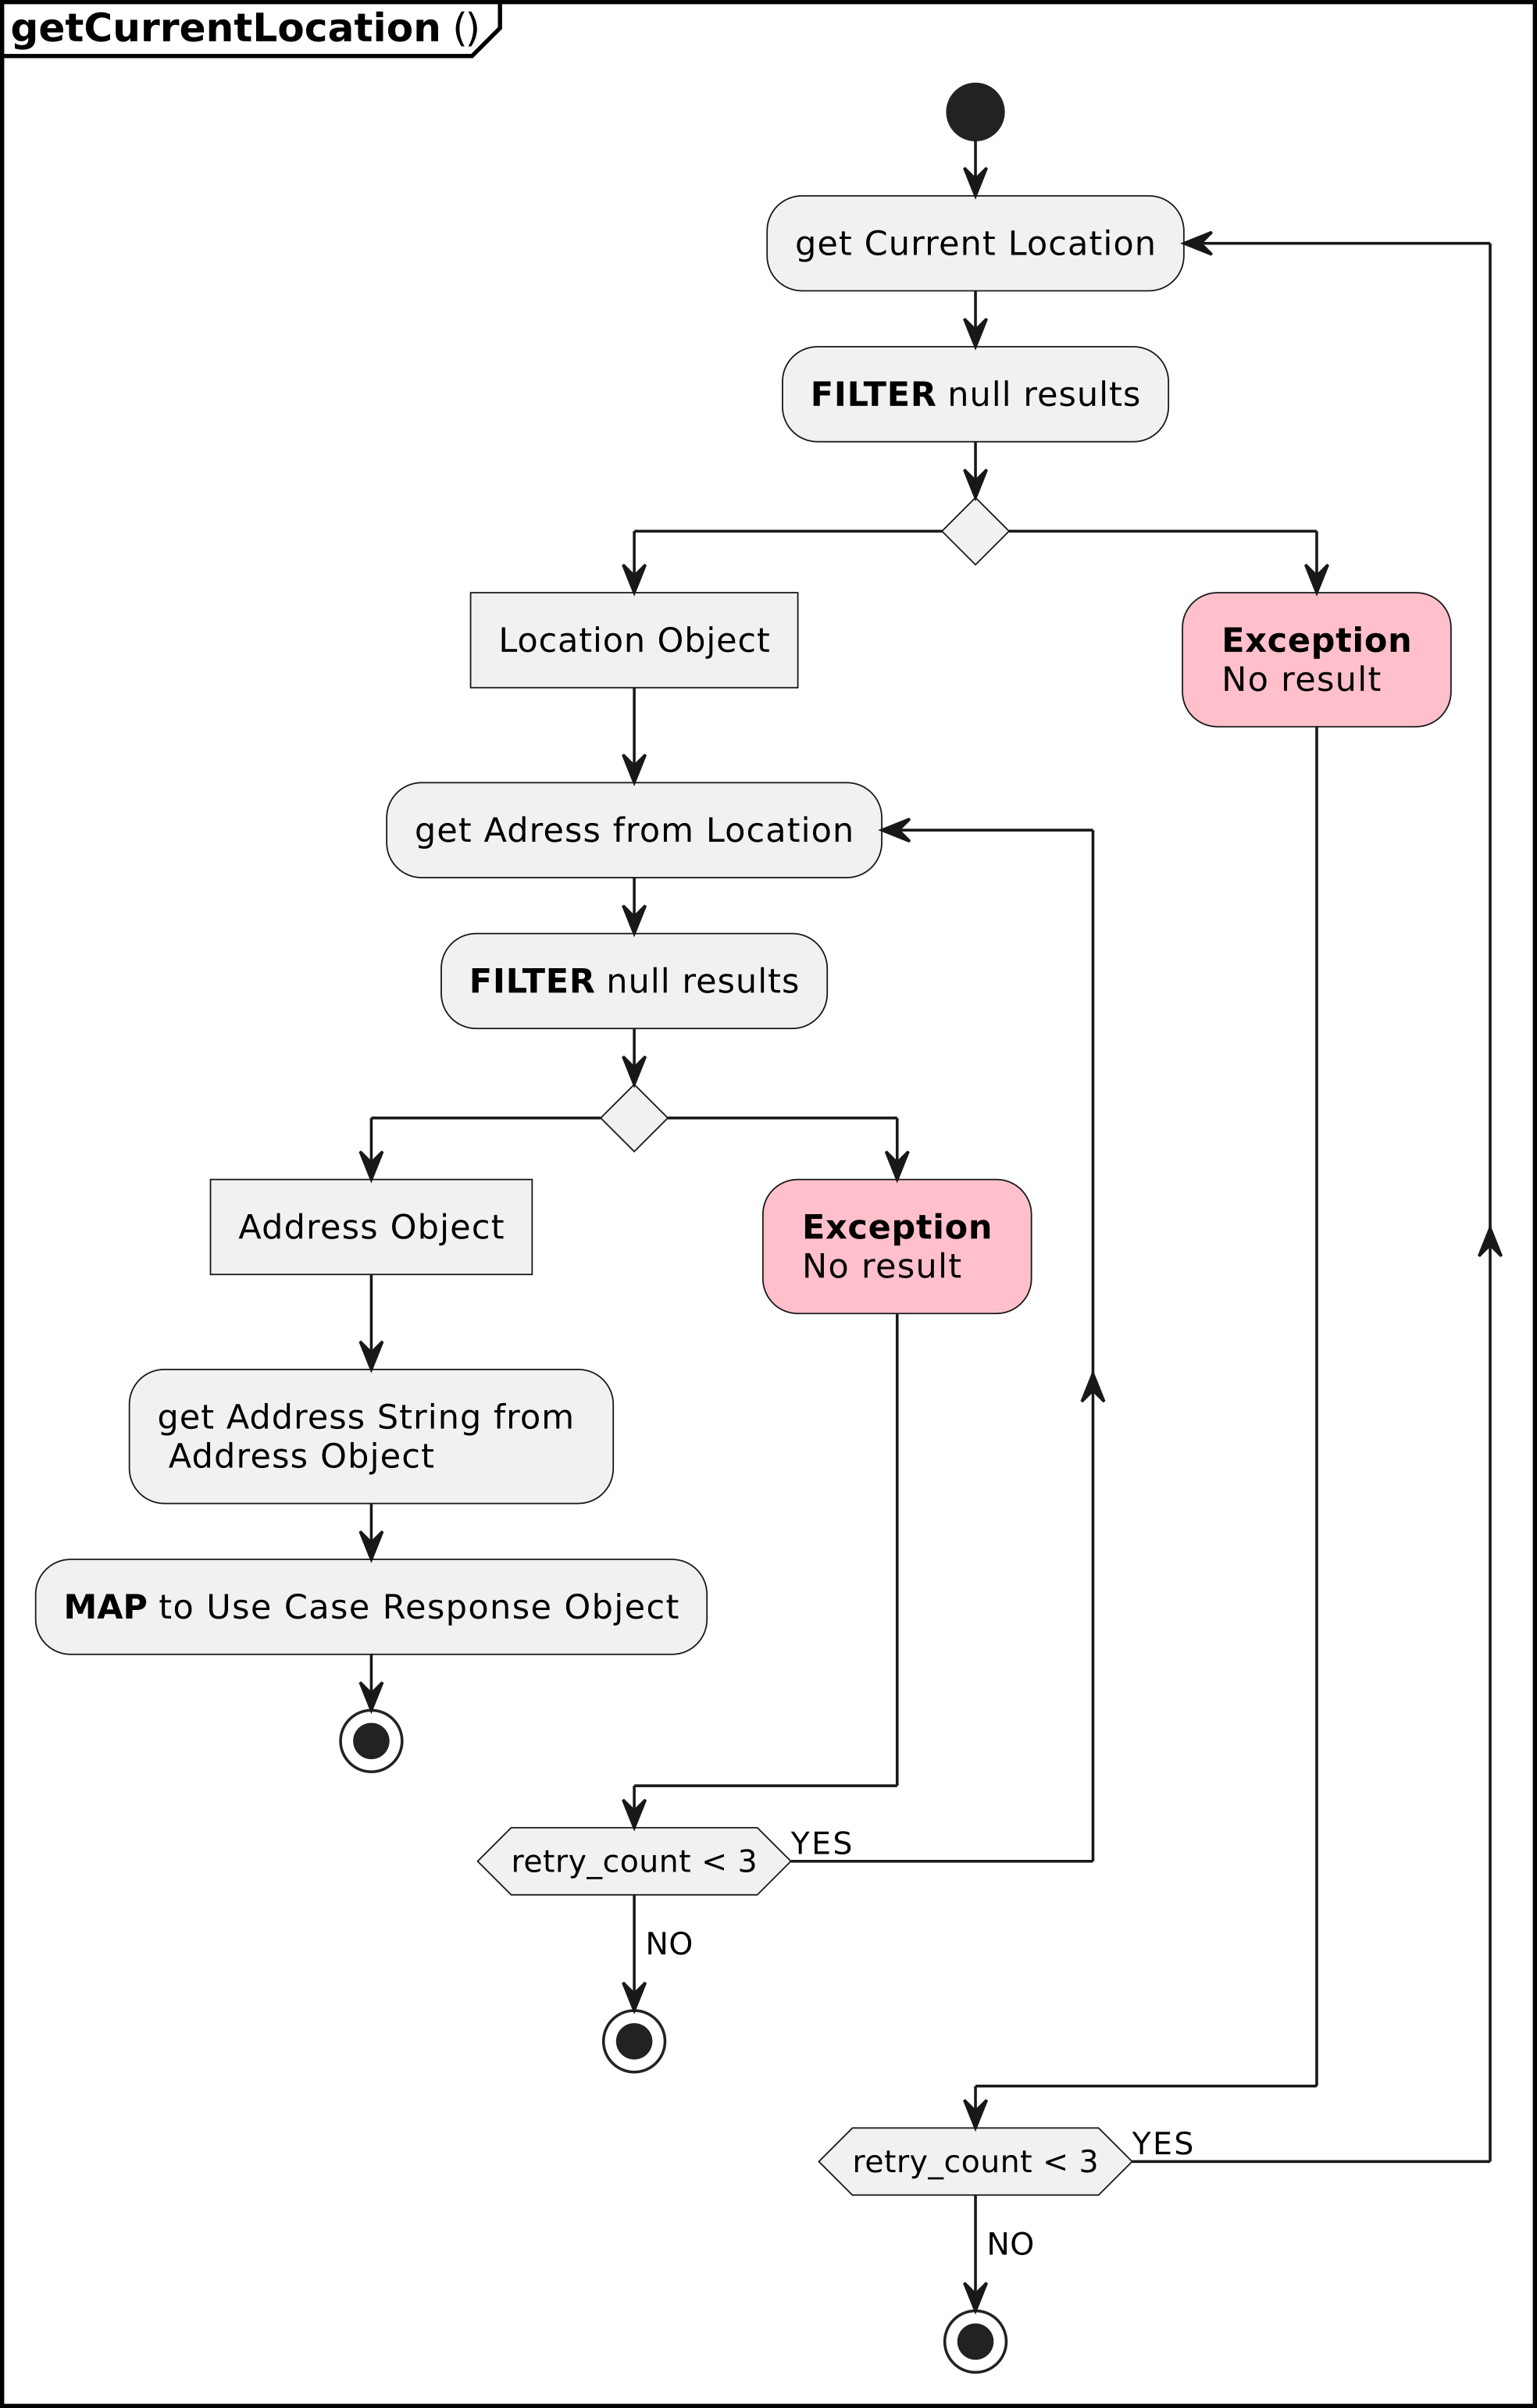
\includegraphics[width=0.8\textwidth]{Figures/iter2/ACT_geoloc.png}
	\rule{35em}{1pt}
	\caption[Class Diagram]{Diagrama de actividades de la implementación del caso de uso: Obtener Geolocalización.}
	\label{fig:act_act_geoloc}
\end{figure}

\subsection{Eliminar Usuario}
Un usuario administrador ingresa a la pantalla de gestión de usuarios de un módulo, sobre la lista de usuarios mantiene presionado el ícono por unos segundos para eliminar un usuario. Se muestra una barra de progreso y la acción termina mostrando un mensaje de éxito o error.
Para esta operación se emplea un único RPC y puede fallar en tres escenarios, a saber:
\begin{itemize}
	\item Error de comunicación con el módulo
	\item El usuario dejó de ser Administrador.
	\item El usuario que se intenta eliminar ya no existe.
\end{itemize}

En el diagrama de la figura ~\ref{fig:act_deleteUser} se puede observar el flujo del algoritmo implementado para este caso de uso.

\begin{figure}[htbp]
	\centering
	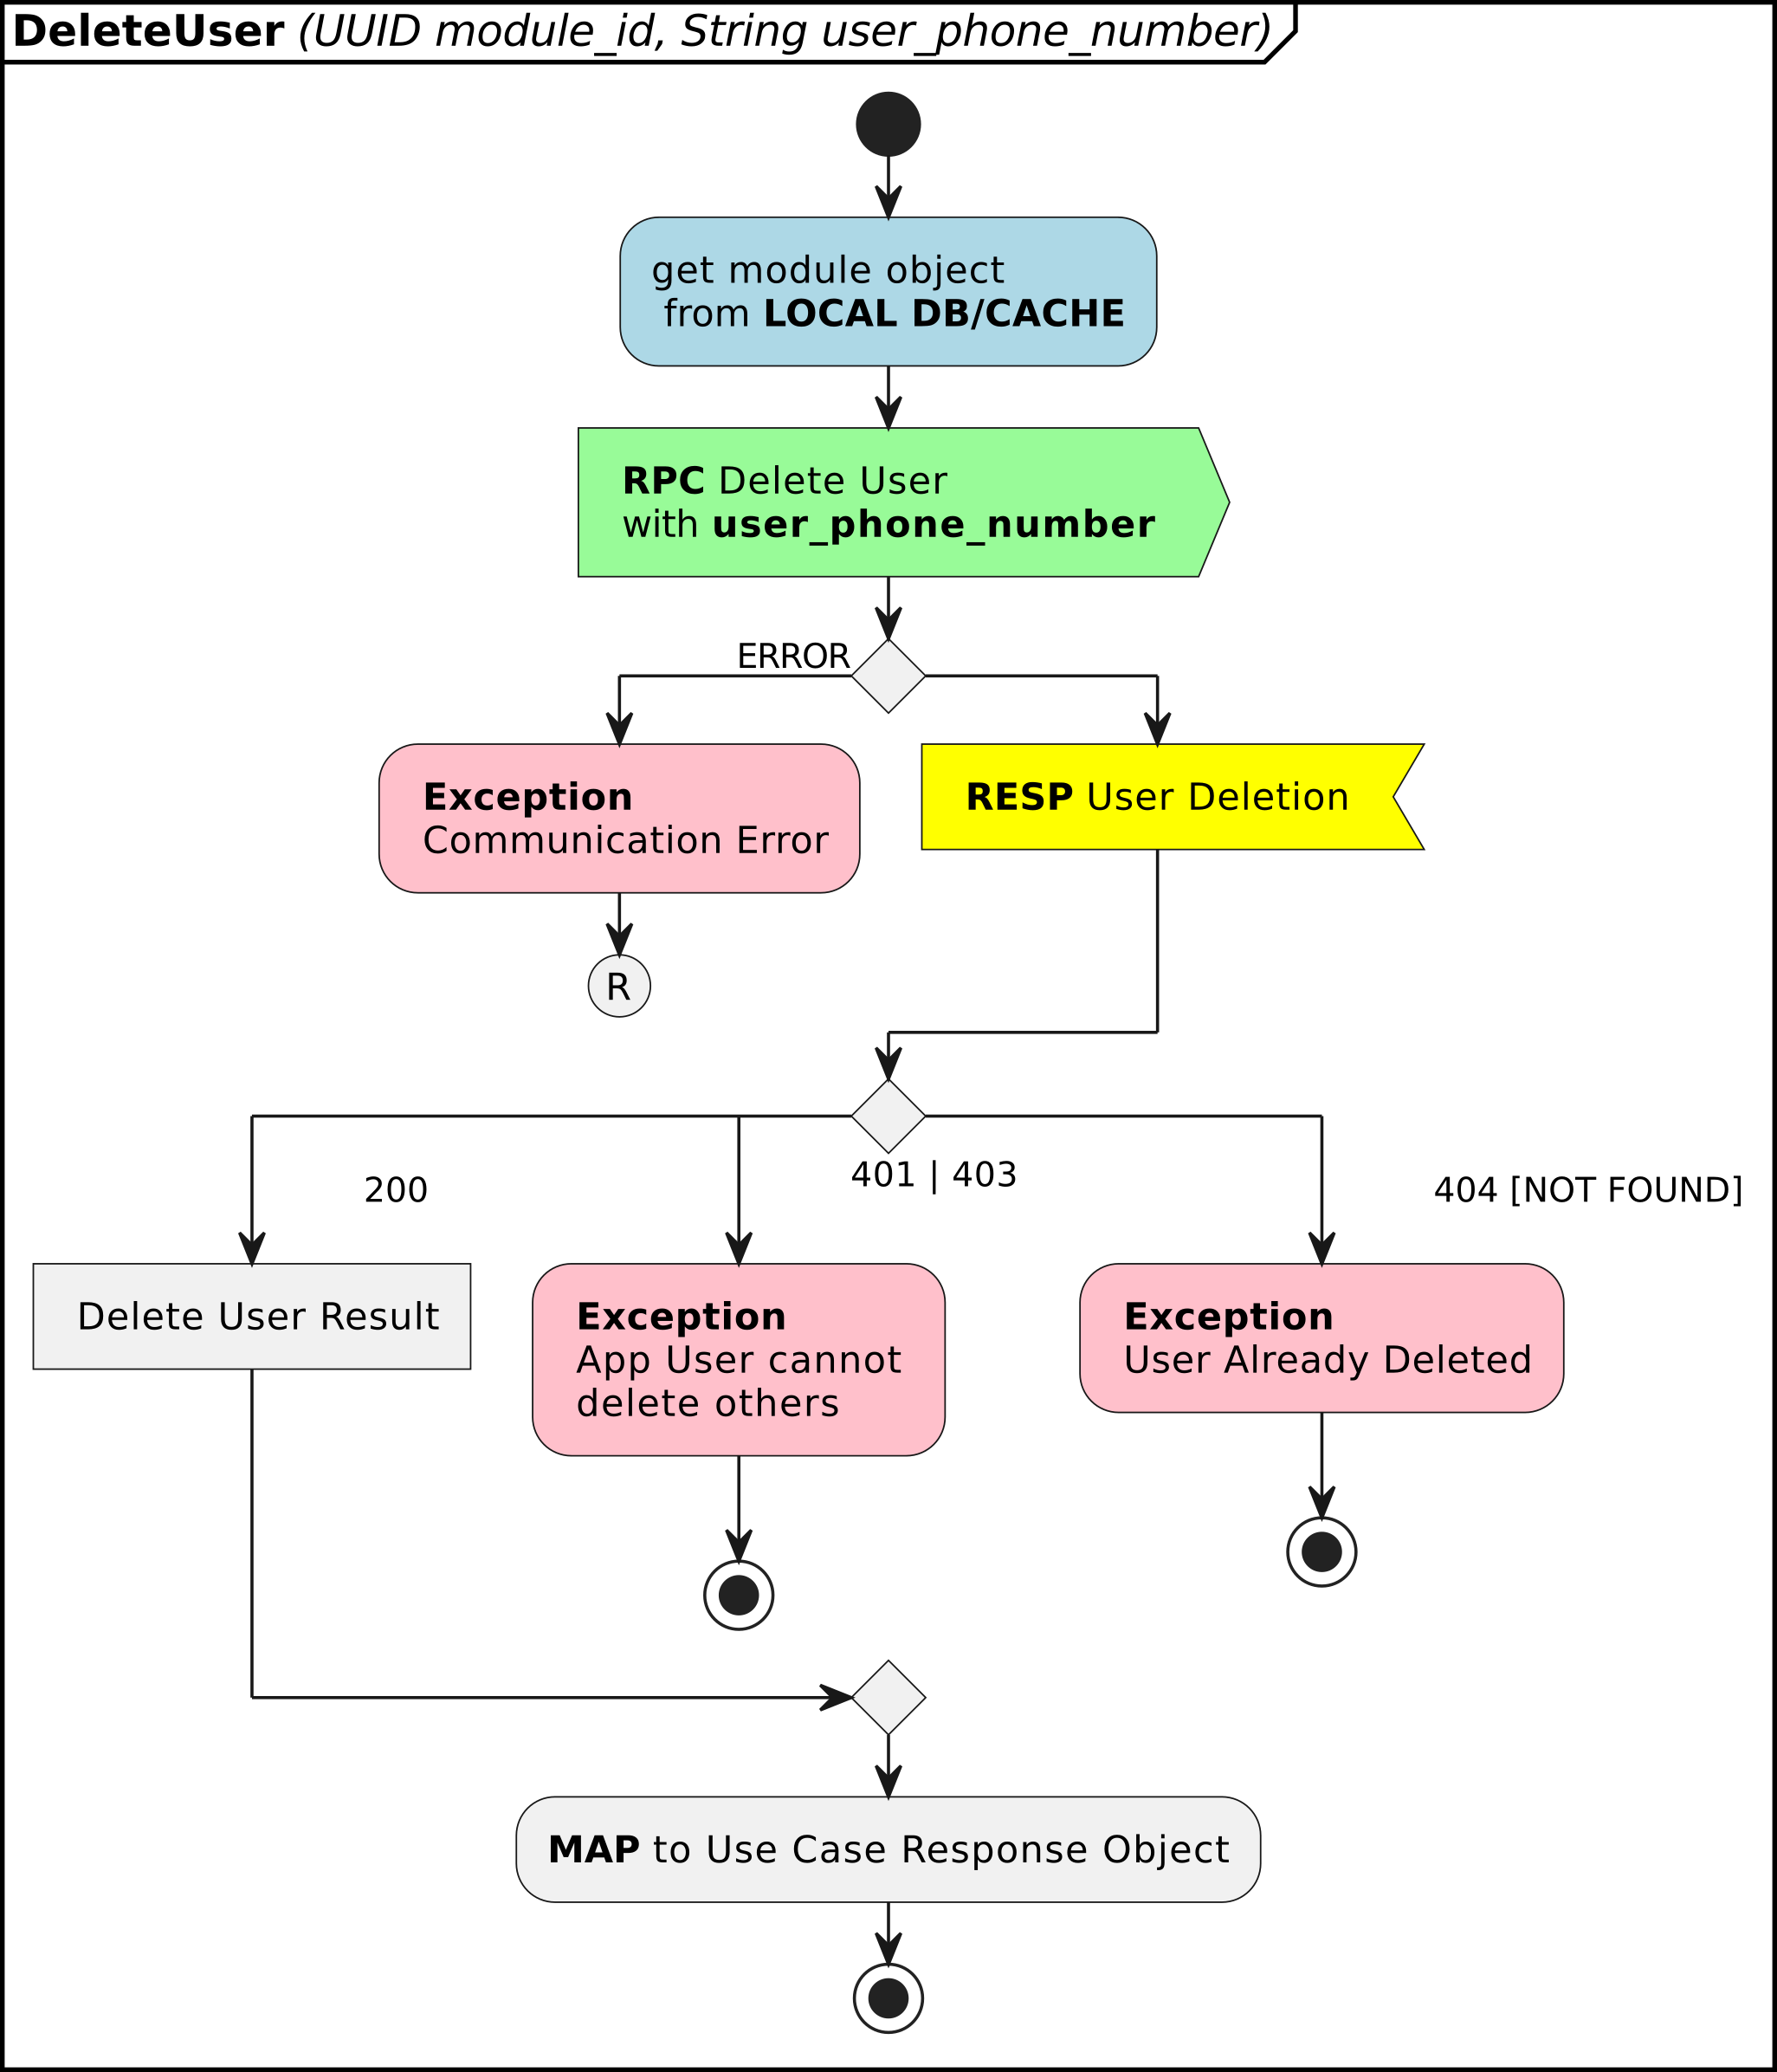
\includegraphics[width=0.8\textwidth]{Figures/iter2/ACT_deleteUser.png}
	\rule{35em}{1pt}
	\caption[Class Diagram]{Diagrama de actividades de la implementación del caso de uso: Eliminar Usuario.}
	\label{fig:act_act_deleteUser}
\end{figure}

\section{Pruebas Automáticas}

\subsection{Dobles de Prueba}
Todo objeto o componente utilizado en las pruebas de software para reemplazar una dependencia real del sistema bajo prueba (SUT: System Under Test). Estos objetos se utilizan para aislar el SUT de sus dependencias, permitiendo un control más preciso sobre las condiciones de la prueba y facilitando la simulación de diferentes escenarios.
Existen diversos tipos de dobles de prueba caracterizados cada uno por el propósito de su empleo en cada caso, a saber:

\begin{itemize}
	\item \textbf{Mock}: Objeto ``maqueta'' que imita la interfaz del objeto dependencia real con el objetivo de simular interacciones con el SUT para dado caso de prueba.
	\item \textbf{Stub}: Trozo de código que se utiliza como sustituto funcional para implementaciones reales con el objetivo de emular precondiciones del caso de prueba.
	\item \textbf{Spy}: Hace referencia a la capacidad de un objeto de verificar la utilización de sus métodos con el propósito de evaluar la ocurrencia de las interacciones del SUT con tal objeto dependencia que determinarán si el caso de prueba pasa son éxito o resulta fallido.
	\item \textbf{Dummy}: Reemplazo de una dependencia que es necesaria para cumplir alguna firma pero que puede ser no utilizada en el caso de prueba.
	\item \textbf{Fake}: Re-Implementación funcional exclusiva de un objeto dependencia empleado por uno o todos los casos de prueba de un SUT. Se utiliza cuando el entorno de pruebas presenta limitaciones o restricciones que hacen necesaria una implementación reducida, simplificada o especializada de dicha dependencia. 
\end{itemize}

Teniendo en cuenta estas definiciones un Mock es un Stub, un Spy y un Dummy. 
Sin embargo un objeto Fake no tiene relación con los otros tipos ya que es una implementación independiente y funcional por si misma que será utilizada solo en el entorno de pruebas para ejecutar los casos de prueba.

Los casos de pruebas unitarias para la aplicación móvil se implementaron utilizando el framework \texttt{JUnit} y la librería \texttt{Mockito} que permite la creación de dobles de prueba de una manera simplificada facilitando su codificación.\\
Aunque \texttt{Mockito} respeta las definiciones de dobles de prueba anteriormente detalladas existe una particularidad en cuanto a la declaración de objetos tipo Spy. La declaración explícita de un Spy en \texttt{Mockito} se realiza sobre la implementación ``real'' de una dependencia agregando el wrapper que permite evaluar la utilización de sus métodos. Así mismo todos los dobles de prueba tipo Mock incorporan la capacidad de un Spy por defecto.

\subsection{RxJava Test}
La librería RXJava ofrece algunas utilidades para evaluar casos de prueba. Entre ellas podemos encontrar a un suscriptor de prueba y un scheduler de prueba.
\begin{itemize}
	\item \texttt{TestSubscriber}: Permite verificar si el stream reactivo terminó correctamente o con error. La cantidad de total de elementos emitidos y comparar el stream con una lista de elementos. 
	\item \texttt{TestScheduler}: Permite emular el paso del tiempo. 
\end{itemize}
Teniendo en cuenta que las partes más relevantes del código fueron implementadas utilizando el paradigma reactivo. Con estas herramientas a disposición es posible conseguir un mayor control sobre la validación de los casos de prueba.

\subsection{Convención de Nombrado}
Se optó por utilizar la convención de nombres para casos de prueba semejante al lenguaje Gherkin. Con esta nomenclatura es posible entender las precondiciones de la prueba (\texttt{Given}), el disparador del caso de prueba (\texttt{When}) y el resultado esperado (\texttt{Then}) con solo leer el nombre del test.
Entonces el nombre de la prueba tendrá el siguiente formato:\\
\texttt{Given\_...\_When\_...\_Then\_...\{\}}

\subsection{Metodología}
Para asegurar la total cobertura de los casos de prueba para las clases y métodos más relevantes se dibujaron los diagramas de actividades correspondientes y se identificaron las ramas condicionales que definen los escenarios de ejecución. Se determina así la complejidad ciclomática y con ello el número total de casos de prueba necesarios para cubrir todos los escenarios.

En la figura ~\ref{} se muestra el diagrama de actividades para el caso de uso se indican las ramas con las líneas numeradas. Para cada línea se codificará un caso de prueba.

\subsection{Pruebas Unitarias}
Teniendo en cuenta la criticidad de los algoritmos implementados para la capa de datos y la lógica de negocios en los casos de uso o capa de dominio. Se escribieron pruebas unitarias para ambas capas. En la figura ~\ref{} se muestra el reporte de ejecución de los casos de prueba. Sobre un total de Se consiguió la ejecución exitosa del total de  
\subsection{Pruebas de Funcionales}
\chapter{Desarrollo: Iteración III} % Main chapter title

\label{Chapter8} % Change X to a consecutive number; for referencing this chapter elsewhere, use \ref{ChapterX}

\steveCabecera{Capítulo 8. \emph{Iteración III}} % Change X to a consecutive number; this is for the header on each page - perhaps a shortened title

%----------------------------------------------------------------------------------------
%	SECTION 1
%----------------------------------------------------------------------------------------
\section{Introducción}
En este capítulo se documentan aspectos relevantes relacionados con la codificación que se realizó en la tercera iteración de desarrollo del software.\\
Aparece un nuevo requerimiento funcional a partir de la devolución de un grupo de early testers quienes solicitaron un modo de accionamiento rápido a través de alguna interfaz en la pantalla de bloqueo de android.
Quizás el cambio más importante introducido en esta iteración es la inclusión del canal de comunicación con los módulos a través de internet. Se describirá el modo de empleo del protocolo MQTT para conseguir la ejecución de los RPC. Se codificó un wrapper reactivo sobre la librería paho de eclipse empleada para configurar el cliente MQTT y su posterior empleo en la aplicación. %%Request Response over Subscribe Queues, message duplicaction,message payload format
Dado que se habilitó un nuevo canal, el repositorio deberá decidir cuando ejecutar los RPC por LAN o Internet, se expondrá el algoritmo utilizado para la selección de los canales.
Finalmente así como se hizo para las iteraciones previas se expondrán las implementaciones más interesantes de la lógica de negocios de los caso de uso planificados para esta iteración.
%% implementaion sofisticada con templates genericos
\section{Accionamiento Rápido}
Luego de producir las primeras unidades del módulo
decidimos distribuirlas a un grupo de usuarios que estaban interesados en probar el producto.
Pasado el período de pruebas nos pusimos en contacto con ellos y tomamos registro de sus devoluciones.
Un comentario común entre la mayoría fue que les parecía que tenían que hacer demasiado para accionar sus portones.
Apareció entonces la propuesta de adicionar un elemento visual en la pantalla de bloqueo de android
que permita el accionamiento sin tener que desbloquear el teléfono.

En la figura ~\ref{fig:notif_design} se puede ver una maqueta de cómo luciría el control rápido implementado como una notificación permanente de android.

Como medidas de seguridad para evitar accionamientos accidentales se propuso limitar los módulos
disponibles para este tipo de accionamiento a aquellos que se encuentren dentro de un radio de 320 metros alrededor del teléfono. También se incluyó un segundo botón que habilita el accionado, obligando al usuario a realizar 2 movimientos voluntarios para completar la acción: tomando como referencia la figura ~\ref{fig:notif_design} será necesario presionar el botón (3) y luego el botón (4).


\begin{figure}[htbp]
	\centering
	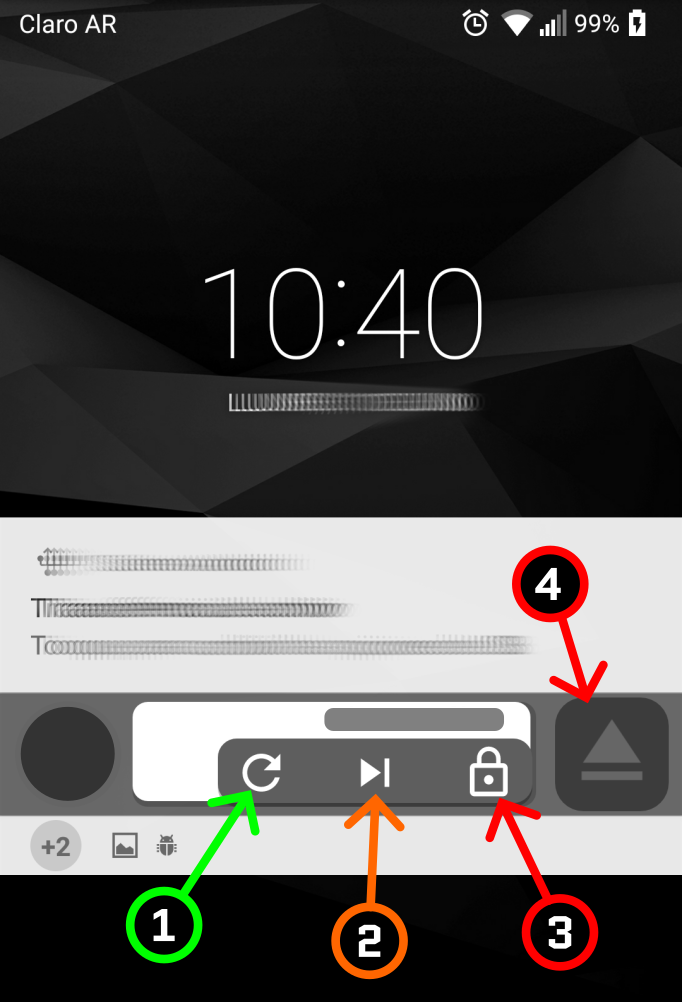
\includegraphics[width=0.4\textwidth]{Figures/iter3/module_notif.png}
	\rule{35em}{1pt}
	\caption[Wireframe]{Maqueta de diseño de la notificación permanente para el control rápido. (1) Botón para buscar los módulos disponibles, (2) Botón para rotar el módulo seleccionado, (3) Botón para habilitar el accionamiento, (4) Botón para accionar el módulo seleccionado.}
	\label{fig:notif_design}
\end{figure}

\section{Canal de comunicación por Internet}
Uno de los aspectos más sobresalientes de la propuesta de valor del producto es la posibilidad
de monitorear, configurar y accionar el módulo de manera remota a través de internet.
En la figura ~\ref{fig:comunic_mod_app} se muestra el esquema de conexión para el modo de operación por internet.
\subsection{Broker MQTT}
Para poder usar el protocolo es necesario contar con un servidor que provea las funciones del broker MQTT.\\
Existen muchas implementaciones listas para usar incluso de código abierto y que se ofrecen de manera gratuita en la red.
De las más populares se optó por un producto chino de nombre \textbf{EMQX}, se trata de una implementación completa del broker MQTT
más un tablero de control y monitoreo web accesible a través del navegador. 
Los autores ofrecen una imagen docker lista para configurar y montar sobre contenedores.
Adicionalmente cuenta con una API HTTP que permite la gestión de tópicos, clientes, sesiones, políticas de acceso y más. Esta implementación también admite el escalado horizontal mediante la configuración de clusters de brokers, estas funcionalidades avanzadas quedan fuera del alcance del presente proyecto.

Para la primera versión del producto se configuró un contenedor de broker EMQX en un servidor virtual privado.
Actualmente EMQX Cloud ofrece un servicio a demanda que no requiere de contar con infraestructura propia.

\subsection{Adaptación del protocolo MQTT}
Como se mencionó en la sección ~\ref{section:mqtt} el protocolo MQTT implementa el patrón de arquitectura Publish-Subscribe .
Sin embargo por definición ~\ref{section:rpc} el protocolo RPC depende de la implementación del patrón Request-Response entre cliente y servidor. 
%sin embargo está claro que la ejecución de protocolos RPC necesita de un canal de comunicación que admita  Request-Response...

Esta controversia se resuelve del lado de la aplicación ofreciendo una adaptación sobre el protocolo MQTT.
Es decir, la suscripción a los tópicos, el envío de mensajes y el formato de los mismos se realizará de manera tal que el modo de comunicación entre aplicación y módulos permita la correcta ejecución de los RPC.

\subsubsection{Formato del Mensaje}
Los mensajes se envían en el payload del paquete MQTT y conservan los formatos descritos para las solicitudes y respuestas descritas en la sección ~\ref{section:rpc} pero para admitir la adaptación necesaria se agregan tres campos extra a saber:
\begin{itemize}
	\item Requester: Es el identificador único del usuario que intenta ejecutar el RPC. Será utilizado por el módulo para autorizar la operación y no se incluye en la respuesta.
	\item Tag: Es la concatenación de los identificadores del módulo y el usuario ejecutor. Este campo se copia sin alterar en la respuesta. Permite a la aplicación identificar el origen de la respuesta.
	\item Id: Es el identificador único del mensaje. Es un número aleatorio que genera la aplicación para cada mensaje con el propósito de detectar duplicados.
\end{itemize}

\begin{multicols}{3} % Change 3 to desired number of columns
	
	% Your content for column 1
	{\small Solicitudes por MQTT:}
	\begin{lstlisting}
{
  "id": 103,
  "method": "method_name",
  "params":{
  "un_parametro": ...,
  "otro_parametro": ...,
  ...
  }

  "requester": 3514123456,
  "tag": "urbit_777::3514123456",
  "id": 2356897
}
	\end{lstlisting}
	
	\columnbreak % Insert a column break between columns
	
	% Your content for column 2
	{\small Respuestas exitosas por MQTT:}
	\begin{lstlisting}
{
  "id": 103,
  "result":{
  "un_resultado": ...,
  "otro_resultado": ...,
  ...
  }
  "tag": "urbit_777::3514123456",
  "id": 2356897
}
	
	\end{lstlisting}
	
	\columnbreak % Insert a column break between columns
	
	% Your content for column 3
	{\small Respuestas con error por MQTT:}
	\begin{lstlisting}
{
  "id": 103,
  "error":{
  "code": 404,
  "message": "... no existe",
  ...
  }
  "tag": "urbit_777::3514123456",
  "id": 2356897
}
	
	\end{lstlisting}
	
\end{multicols}

\subsubsection{Tópicos y Suscripciones}
\textbf{EJECUCIÓN RPC}

Todos los módulos conectados al Broker MQTT estarán suscritos a un único tópico con el siguiente formato:
\textbf{\texttt{urbit-??????/request}}\\
Los signos de interrogación corresponden al UID de cada módulo. En este tópico recibirá las solicitudes de ejecución de RPC.

Al mismo tiempo publicarán las respuestas a los tópicos generados para cada usuario que respetan el siguiente formato:\\
\textbf{\texttt{urbit-??????/response/XXXXXXXXXX}}\\
Los signos de interrogación corresponden al UID de cada módulo y las equis al UID del usuario. En este tópico se publican las respuestas a las solicitudes de ejecución de RPC.

Los módulos publicarán los cambios en el estado de apertura a el tópico con el siguiente formato.
\textbf{\texttt{urbit-??????/status}}\\

\textbf{INVITACIONES}

Cuando un administrador crea un usuario a partir de su número telefónico en la pantalla de gestión de usuarios. El módulo publica su propio identificador como mensaje retenido en un tópico especial que permite que el usuario invitado pueda encontrar de manera remota este nuevo módulo al que se le a cedido acceso.
Estos tópicos de invitaciones respetan el siguiente formato:\\
\textbf{\texttt{XXXXXXXXXX/invitation/urbit-??????}}\\
Donde las equis corresponden al identificador del usuario invitado y los signos de interrogación al identificador del módulo.

Dado que un usuario puede ser invitado a operar diversos módulos resulta sumamente útil emplear los ``wildcards'' admitidos por MQTT para nombres de tópicos y que permiten suscripciones múltiples. La aplicación cliente se suscribe a un tópico con el siguiente formato:
\textbf{\texttt{XXXXXXXXXX/invitation/+}}\\
Donde las equis corresponden al identificador del usuario y el signo de suma es el comodín que habilitará la recepción de invitaciones de cualquier módulo.

\subsection{RPC sobre MQTT}
Al momento de ejecutar un RPC la aplicación cliente genera el mensaje con el formato indicado anteriormente y lo publica al tópico de solicitudes del módulo. El módulo al recibirlo realizará la tarea de autorización, ejecutará el procedimiento correspondiente y publicará el resultado en el tópico de respuestas.
En la figura ~\ref{fig:act_publish_rpc} se muestra el procedimiento completo de envío de la solicitud de ejecución y la resepción de la respuesta.
El algoritmo puede fallar en 3 escenarios a saber:
\begin{itemize}
	\item Error de conexión al Broker.
	\item Error al momento de Publicar el mensaje.
	\item El timeout fijado para la operación fue excedido sin registrar respuestas.
\end{itemize}

\begin{figure}[htbp]
	\centering
	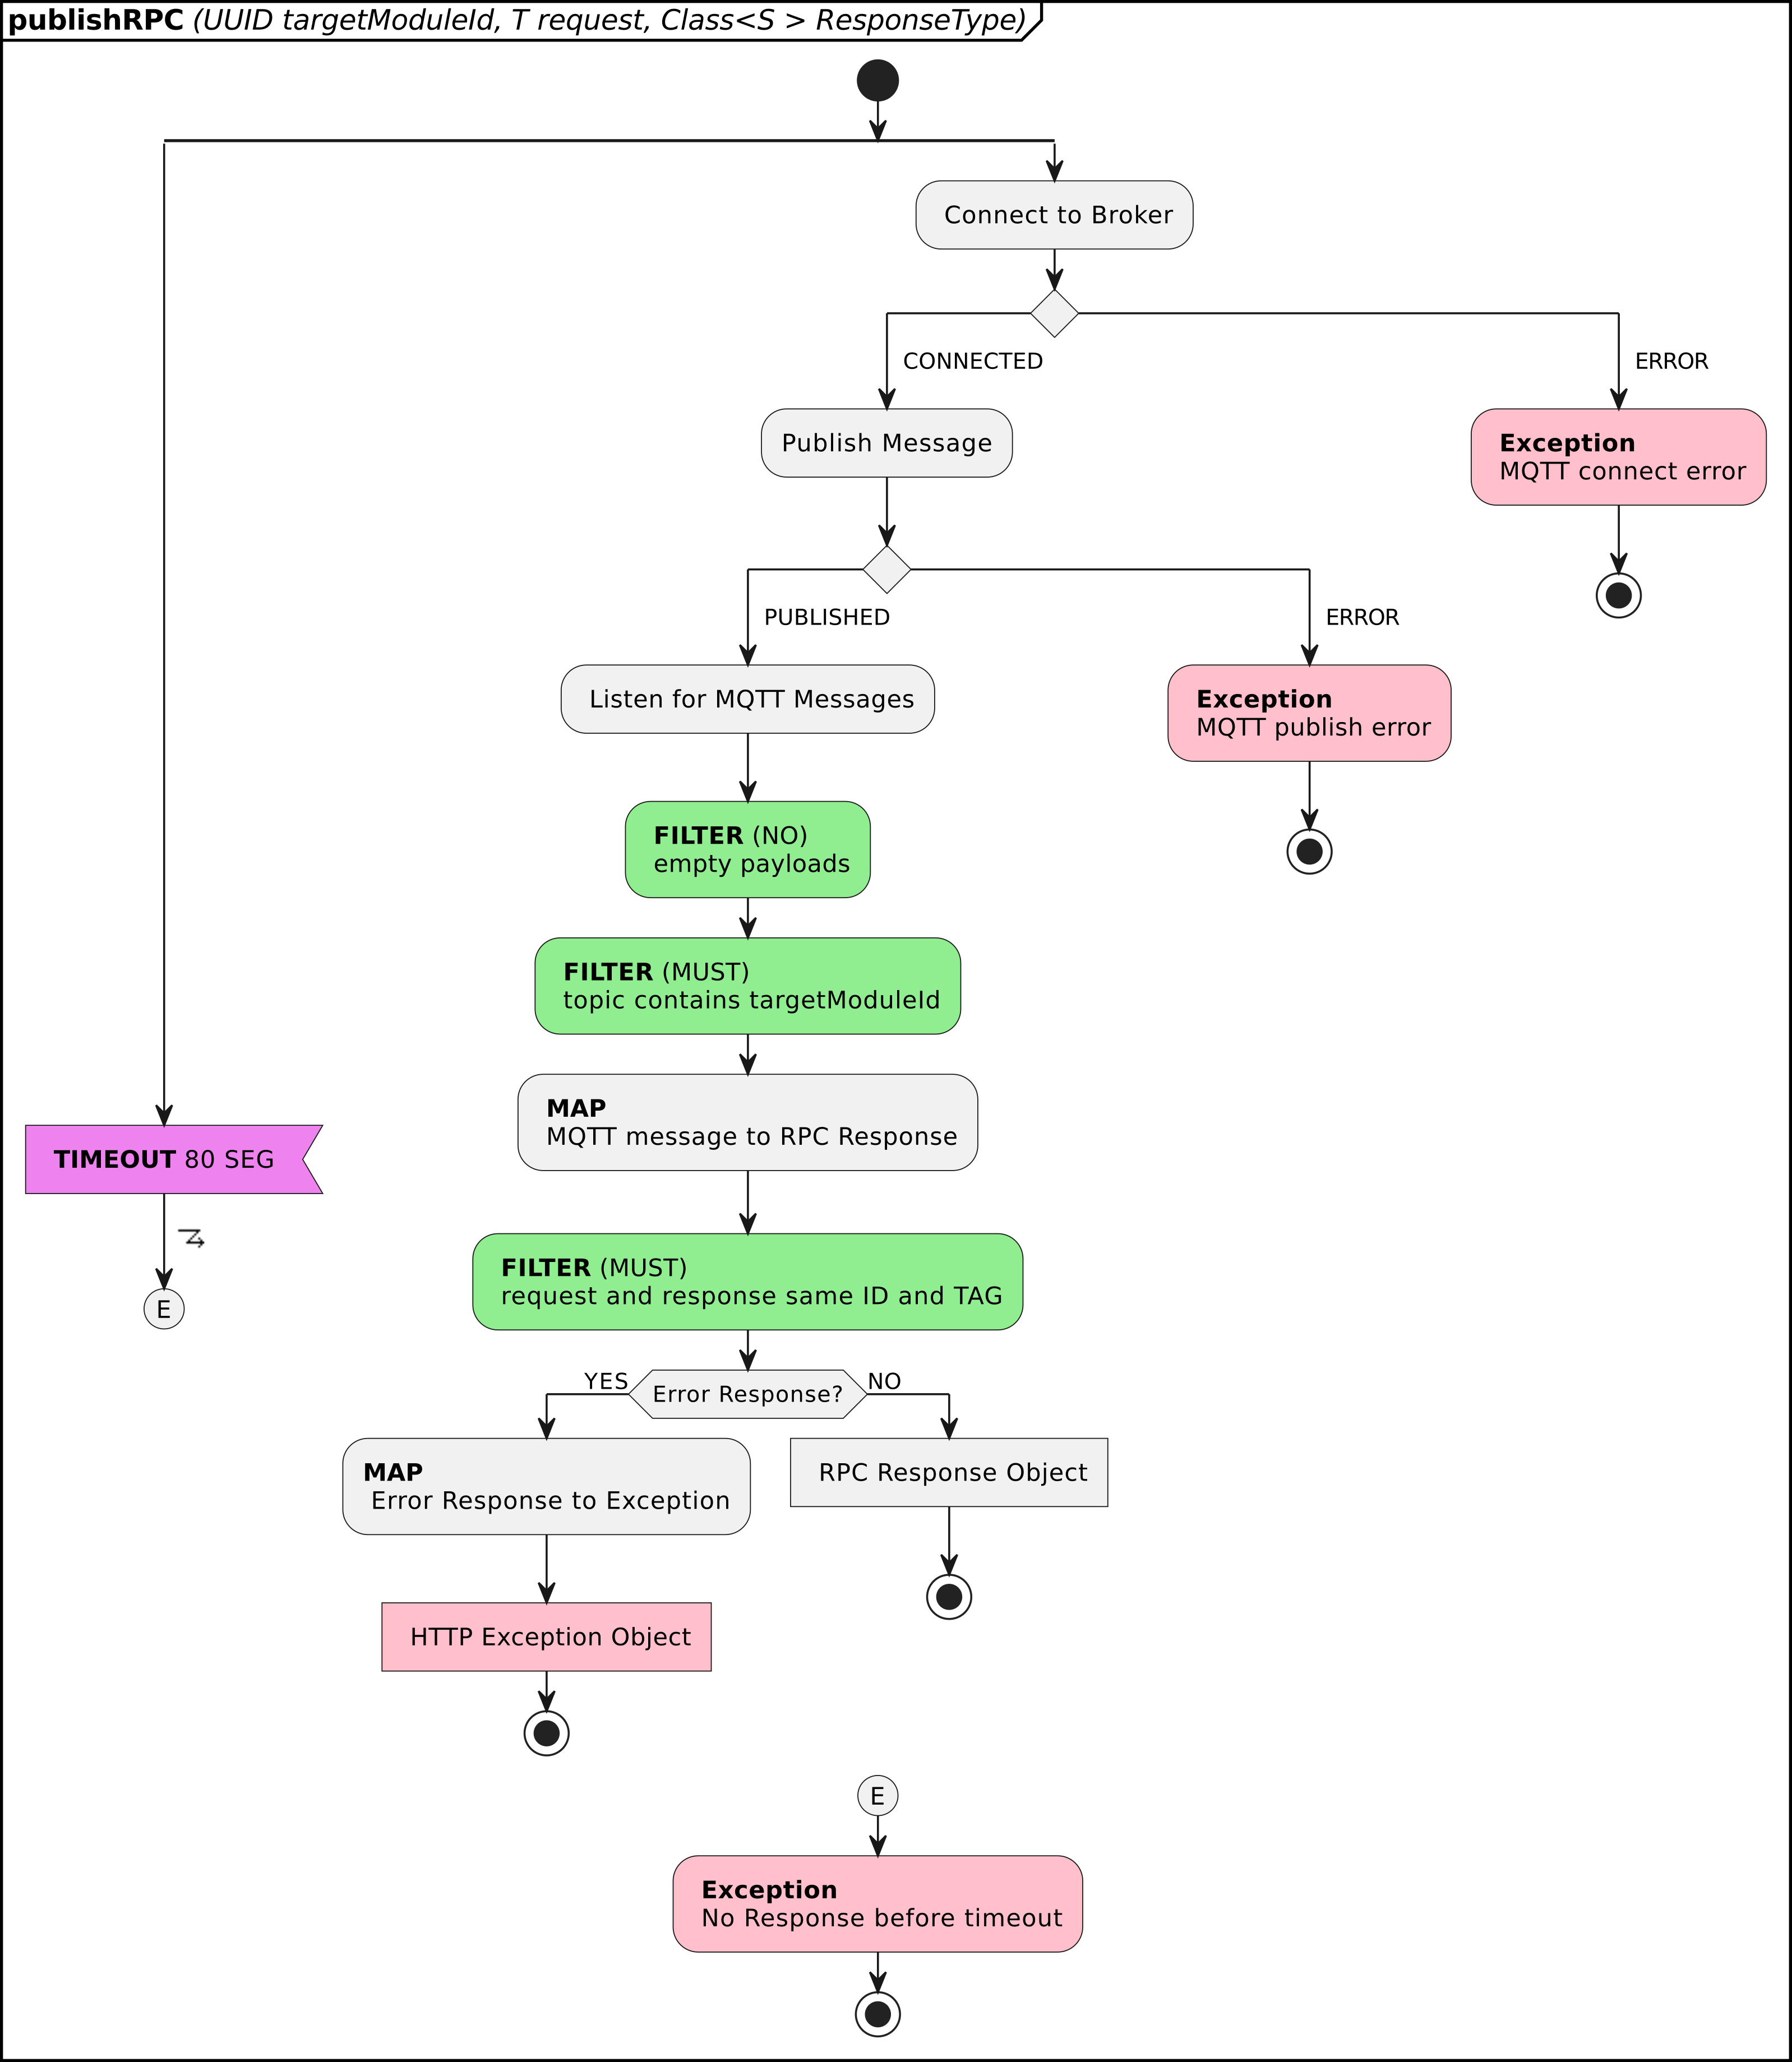
\includegraphics[width=0.9\textwidth]{Figures/iter3/ACT_publishRPC_ink.png}
	\rule{35em}{1pt}
	\caption[UML Diagram]{Diagrama de actividades del procedimiento de envío de una solicitud y recepción de la respuesta al momento de ejecutar un RPC.}
	\label{fig:act_publish_rpc}
\end{figure}

Existe un escenario que produce une excepción pero que no representa un fallo de la rutina sino que se genera a propósito como un mapeo de la respuesta de operación no exitosa enviada por el módulo y así conservar la compatibilidad con los casos de uso ya implementados.


\subsection{Selector de Canales}
Al introducir un nuevo canal de datos por el cual se pueden ejecutar los procedimientos remotos se hizo necesario incorporar una rutina que decida cuál es el canal apropiado para realizar la operación conforme a las condiciones de conexión del teléfono.
\subsubsection{Ejecutor}
Para resolver la tarea y teniendo en cuenta la similaridad de todos los métodos asociados a la ejecución de RPC, se optó por codificar una clase interna al repositorio denominada \texttt{RPCExecutor}. Esta clase se implementó utilizando tipos genéricos de Java ya que cada RPC utiliza objetos solicitud y respuesta de tipos únicos. \texttt{RPCExecutor} permite generalizar el modo de ejecución de los RPC de manera que el codigo en cada uno es equivalente.
Se declara un método de nombre \texttt{executeRPC} que hace uso del ejecutor para decidir la fuentes de datos primaria, con la que intentará ejecutar el procedimiento en caso de fallar intentará con la segunda si es que está disponible.
El orden de prioridad de estas fuentes de datos se determina en un método aparte denominado getDataSourceChoices. En la figura ~\ref{fig:act_choices} se muestra el algoritmo utilizado. El estado de conexión de teléfono se obtiene usando las APIs provista por el SDK de android.

\begin{figure}[htbp]
	\centering
	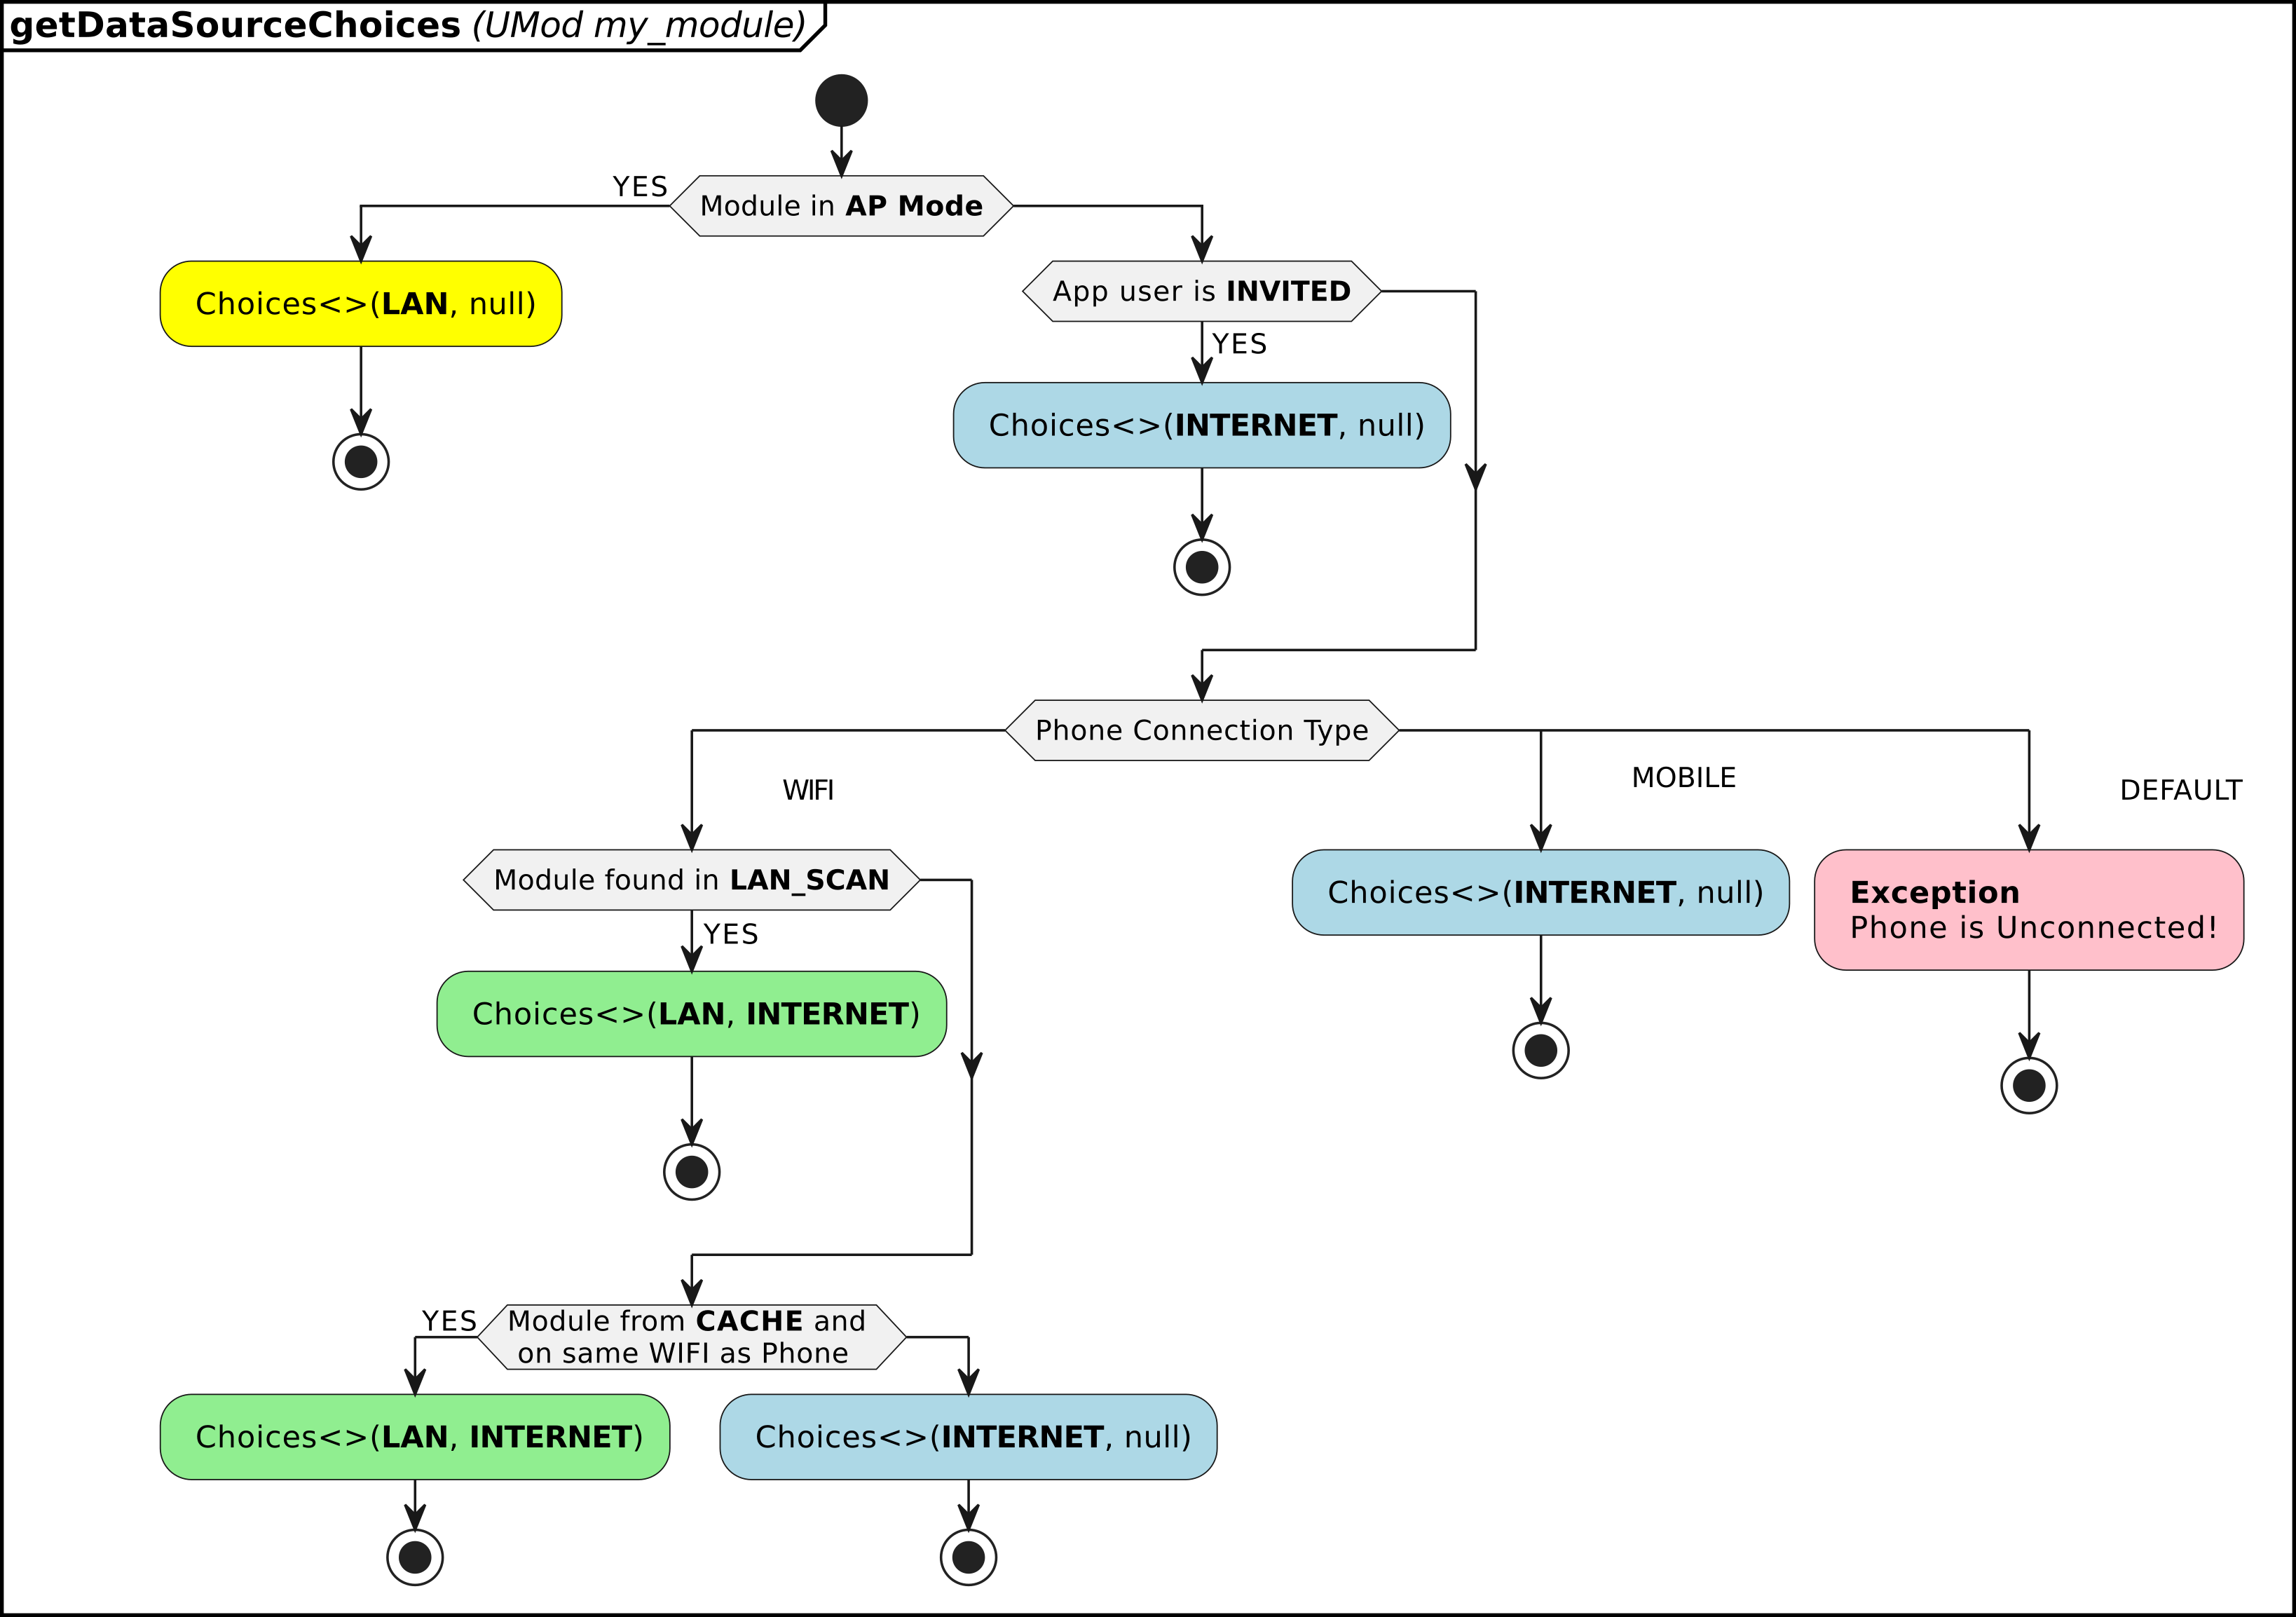
\includegraphics[width=0.9\textwidth]{Figures/iter3/ACT_choice_ink.png}
	\rule{35em}{1pt}
	\caption[UML Diagram]{Diagrama de actividades del procedimiento que determina el orden de prioridad de las fuentes de datos para la ejecucuín de RPC.}
	\label{fig:act_choices}
\end{figure}



\section{Casos de Uso Implementados}
Para la presente iteración se implementaron los siguientes casos de uso.
\begin{enumerate}
	\item Actualizar GATE-STATUS de los módulos.
	\item Activar Acceso Rápido.
	\item Actualizar Firmware
	\item Habilitar Módulo para Acceso Rápido.
	\item Accionar módulo cercano.
	\item Obtener módulos disponibles para acceso rápido.
	\item Desbloquear botón contra accionamiento accidental.
\end{enumerate}

A continuación se documentaran aquellos que presentan los escenarios más interesantes.

\subsection{Actualizar Firmware}
Este caso de uso es fundamental para garantizar la calidad del producto al proveer actualizaciones para el firmware del módulo.
El usuario administrador ingresa a la pantalla de configuración de un módulo, luego toca el botón asignado para esta operación, acepta el cartel de advertencia y espera hasta que concluya el procedimiento.
Como una nota al margen se menciona que por restricciones impuestas en el framework utilizado para programar el firmware del módulo la actualización OTA solo puede realizarse por el canal LAN y consiste de los siguientes pasos:
\begin{enumerate}
	\item El teléfono descarga un archivo .zip que corresponde a la nueva versión del firmware para el módulo.
	\item El teléfono envía este archivo al módulo mediante un POST HTTP multiparte a un endpoint predefinido que incluye el archivo del nuevo firmware y el valor \texttt{COMMIT\_TIMEOUT} que determina la cantidad de tiempo en segundos que esperará el módulo para que el usuario autorice la nueva versión luego de concluida la instalación y el reinicio exitoso.
	\item El teléfono espera que el módulo se reinicie y ejecuta el RPC GetSysInfo para corroborar la correcta versión del firmware recién instalado.
	\item COMMIT: El teléfono hace un POST HTTP a un endpoint predefinido para autorizar la actualización.
\end{enumerate} 

Este caso de uso utiliza hasta tres RPC en su ejecución y puede fallar en 8 escenarios distintos a saber:

\begin{enumerate}
	\item Error de comunicación con el módulo.
	\item Versión actual del firmware DESCONOCIDA.
	\item Actualización no necesaria.
	\item Error con la URL de descarga del archivo de firmware.
	\item El archivo descargado está vacío.
	\item Error de comunicación con el servidor.
	\item Error de versión después de actualizar.
	\item Error de COMMIT.
\end{enumerate} 

En el diagrama de la figura ~\ref{fig:act_ota} se puede observar el algoritmo implementado para este caso de uso.

\begin{figure}[htbp]
	\centering
	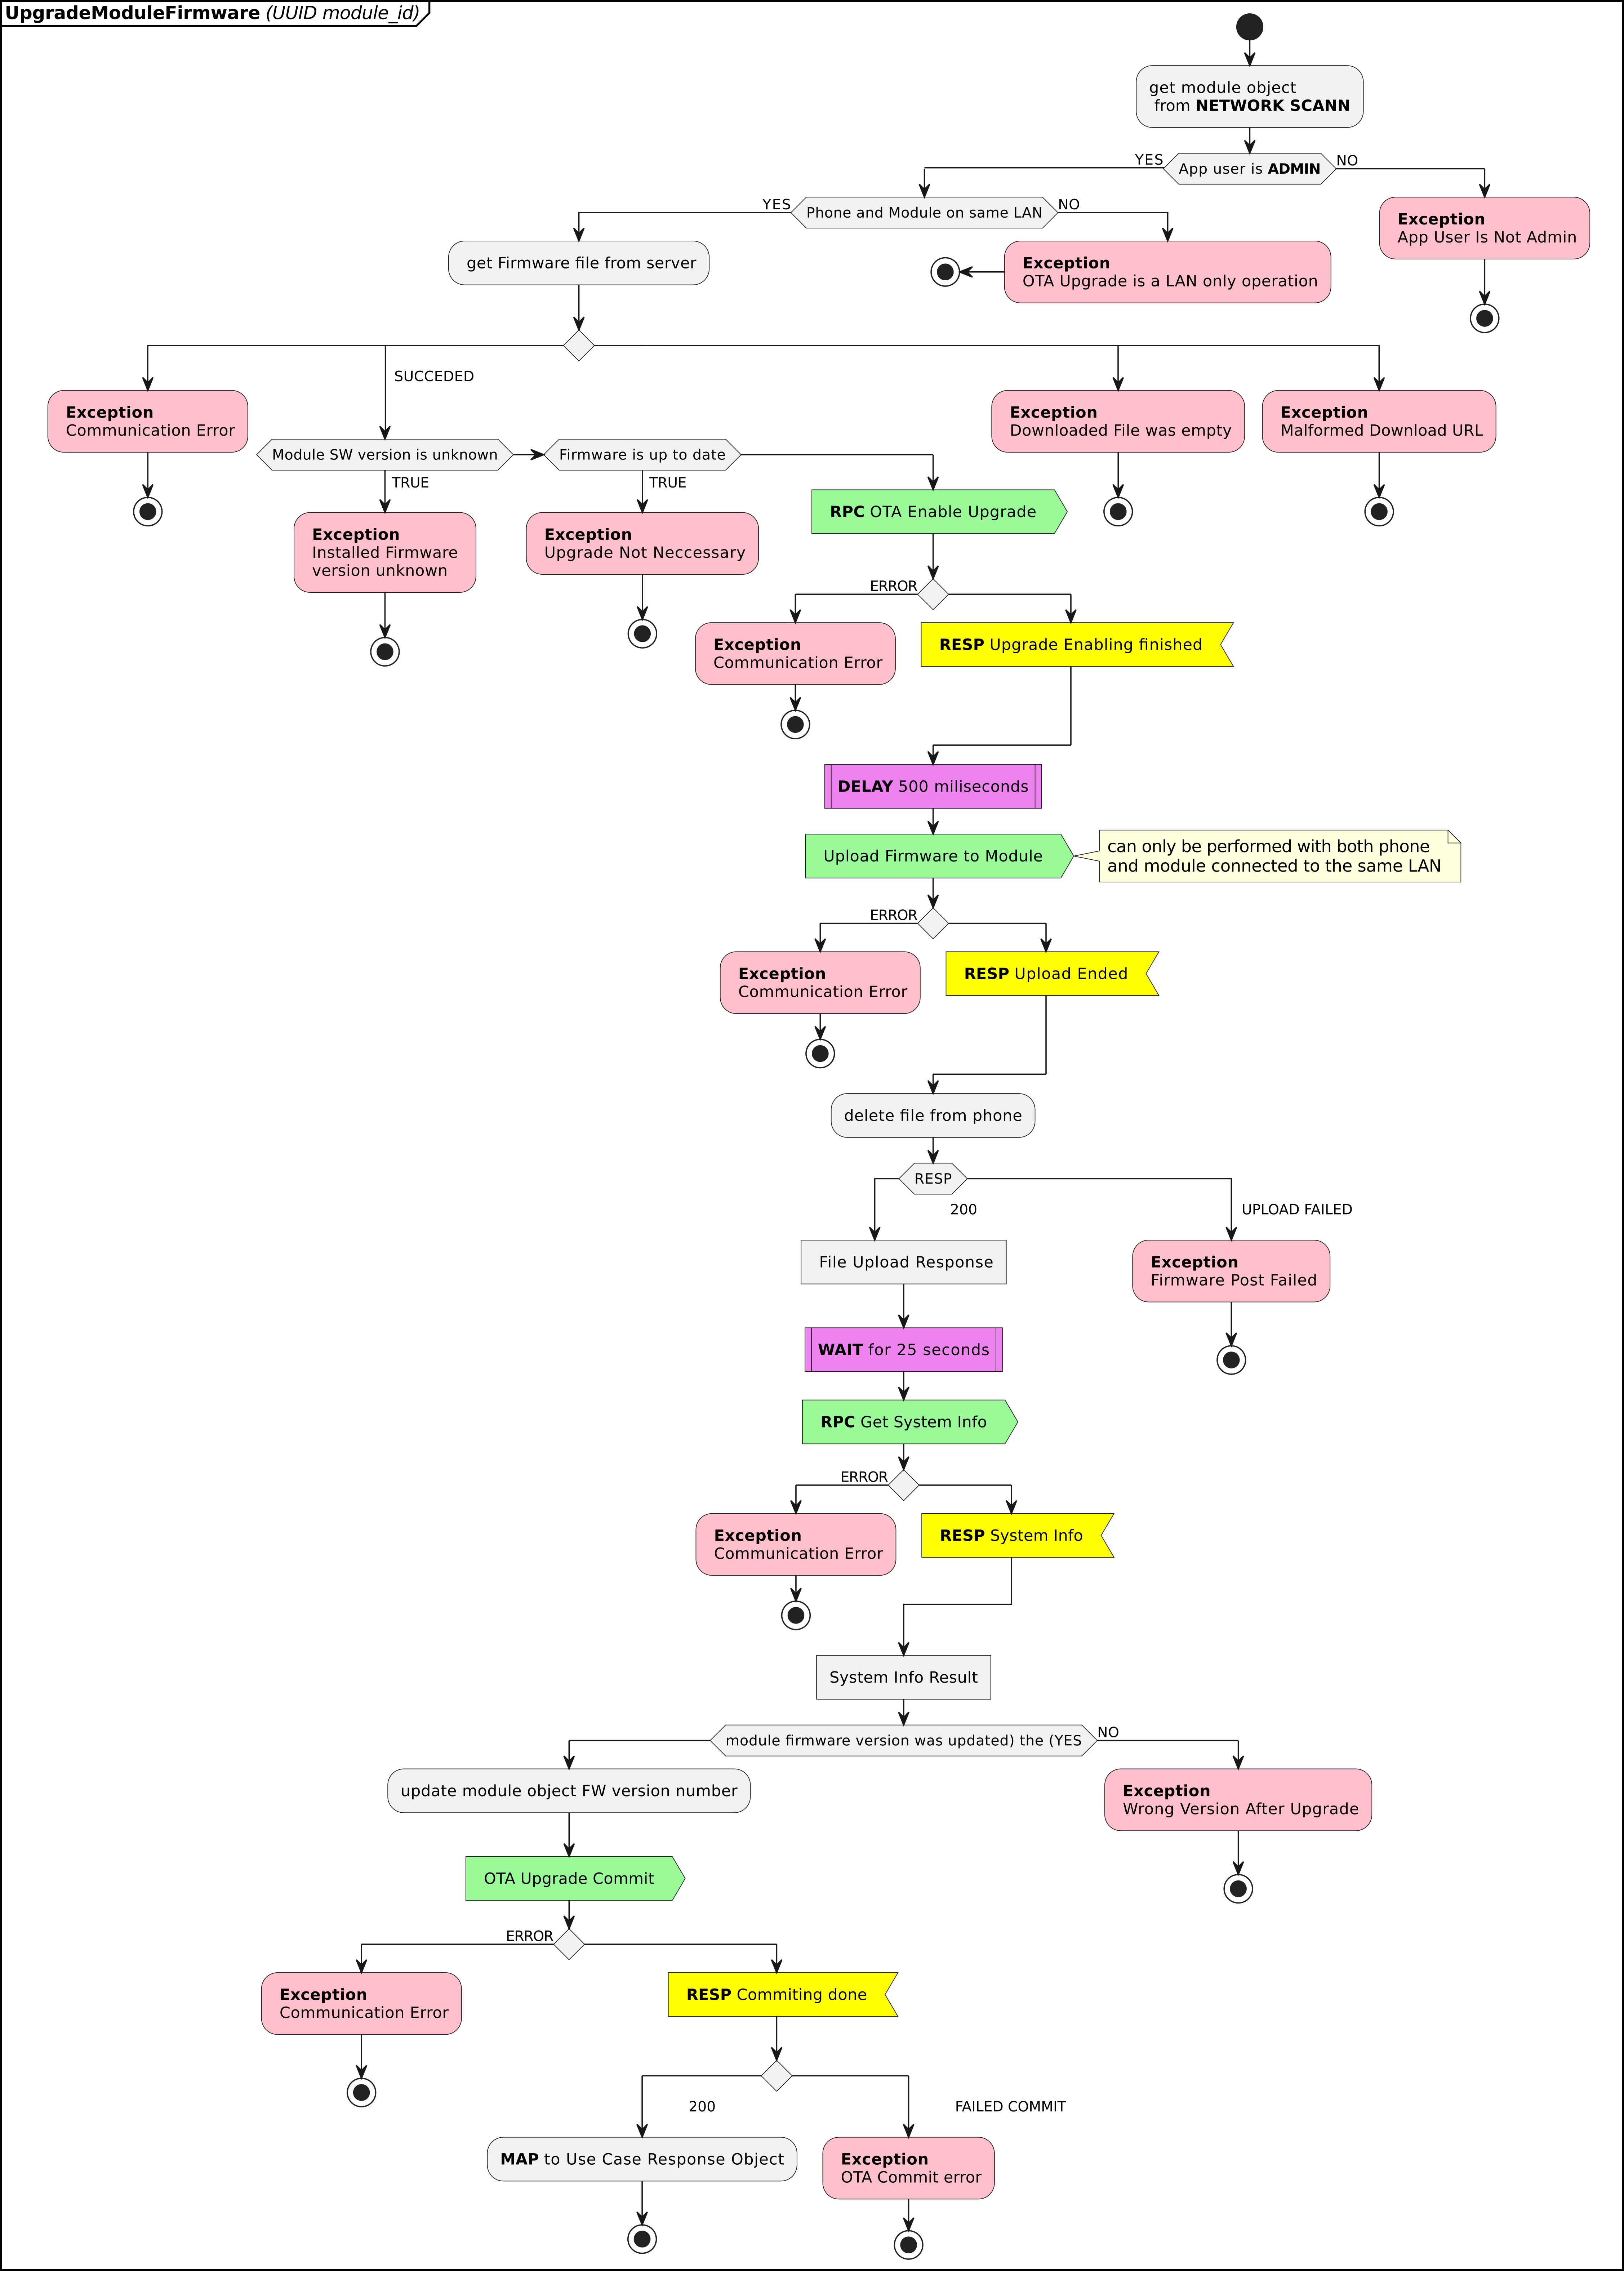
\includegraphics[width=\textwidth]{Figures/iter3/ACT_ota_ink.png}
	\rule{35em}{1pt}
	\caption[Class Diagram]{Diagrama de actividades de la implementación del caso de uso: Actualización de Firmware.}
	\label{fig:act_ota}
\end{figure}

\subsection{Obtener módulos disponibles para acceso rápido}
En la pantalla de bloqueo del teléfono sobre la notificación permanente el usuario presiona
el botón para refrescar los módulos disponibles para accionamiento rápido.
Este caso de uso obtiene la ubicación geográfica del teléfono que debe tener una precisión menor a 60 metros
y su última actualización no debe superar los 5 minutos.
Una vez conocida la posición geográfica del teléfono buscará todos los módulos que cumplan las siguientes condiciones:
\begin{itemize}
	\item El modulo debe estar en STATION\_MODE.
	\item El usuario de la app debe estar autorizado.
	\item El modulo debe tener habilitado el control rápido.
	\item El módulo debe encontrarse a menos de 320 metros de distancia.
\end{itemize}
Este caso de uso no realiza llamadas a RPCs y puede fallar en 8 escenarios.
En la figura ~\ref{fig:act_notif_modules} se puede observar el diagrama de actividades de la implementación del caso de uso.

\begin{figure}[htbp]
	\centering
	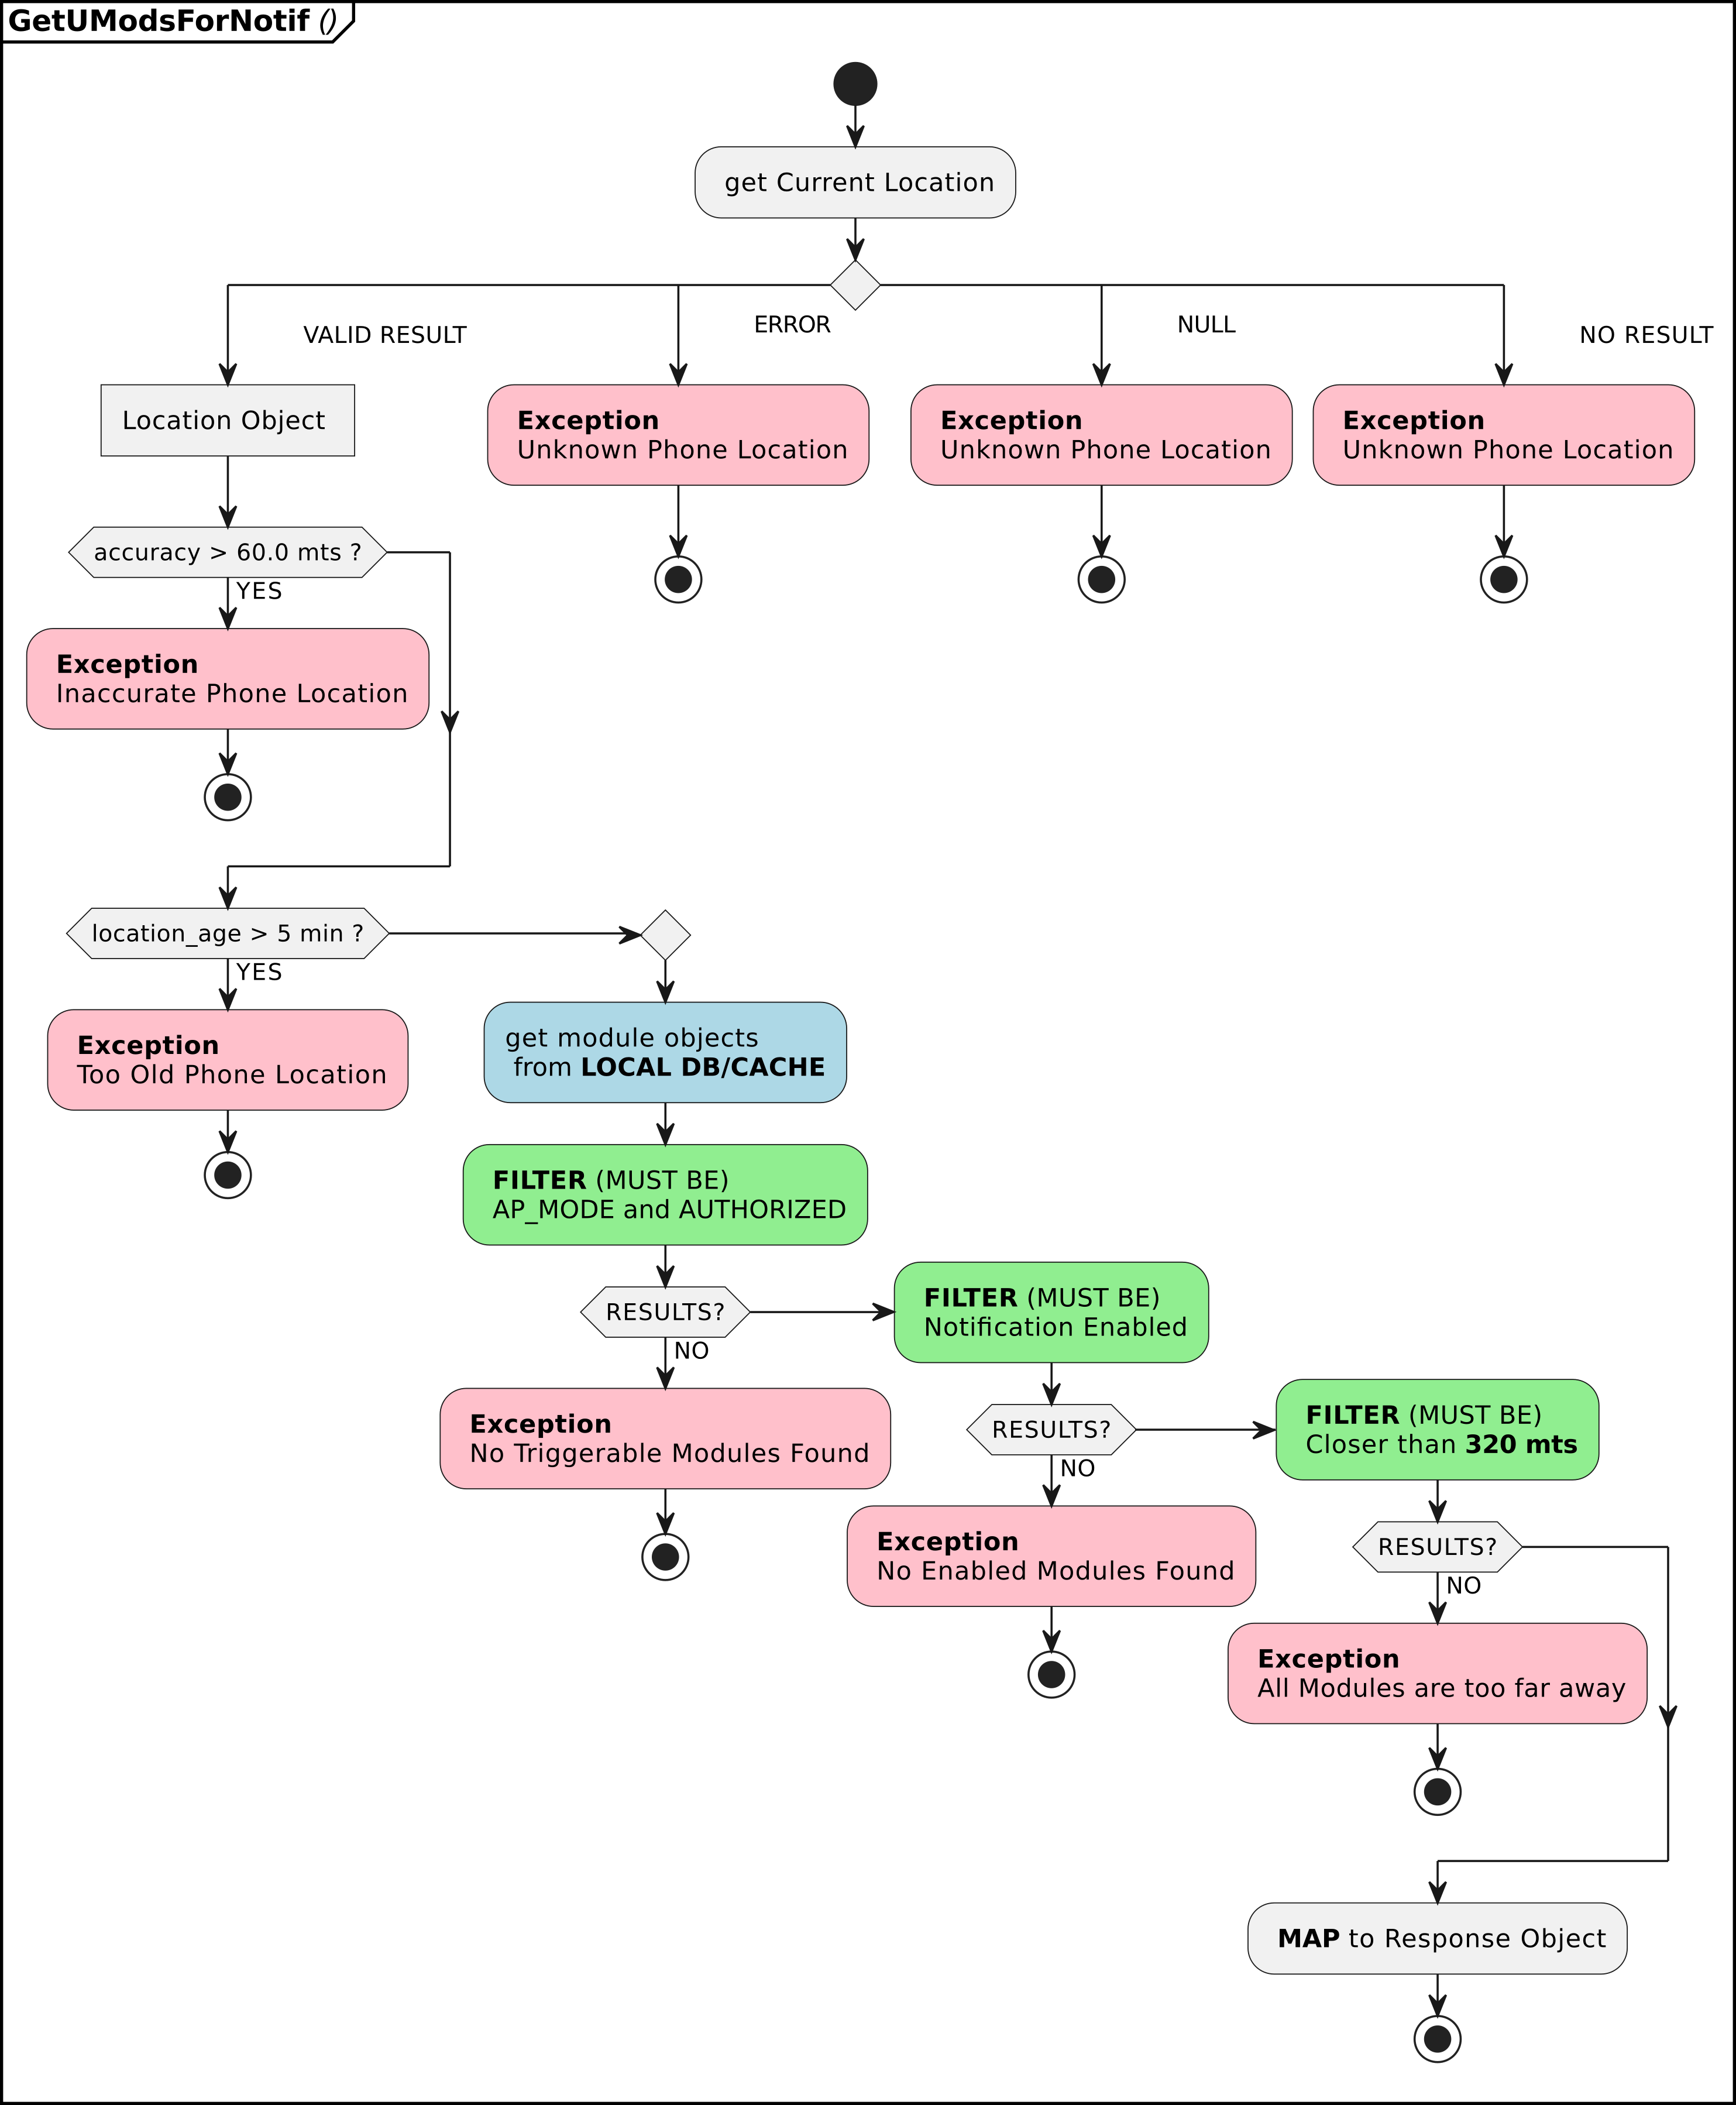
\includegraphics[width=0.8\textwidth]{Figures/iter3/ACT_getModsNotif.png}
	\rule{35em}{1pt}
	\caption[Class Diagram]{Diagrama de actividades de la implementación del caso de uso: Obtener módulos disponibles para acceso rápido.}
	\label{fig:act_notif_modules}
\end{figure}


% Chapter Template

\chapter{Conclusiones y Trabajos Futuros} % Main chapter title

\label{Chapter13} % Change X to a consecutive number; for referencing this chapter elsewhere, use \ref{ChapterX}

\steveCabecera{Capítulo 13. \emph{Conclusiones y Trabajos Futuros}} % Change X to a consecutive number; this is for the header on each page - perhaps a shortened title

%----------------------------------------------------------------------------------------
%	SECTION 1
%----------------------------------------------------------------------------------------
\section{Conclusión}
Al finalizar el proyecto se obtuvo una aplicación android que implementa los casos de uso documentados y cumple con los requerimientos del producto. 
La realización de este proyecto en particular implicó un amplio conocimiento sobre los diversos protocolos y estándares de comunicación involucrados en su funcionamiento.
 
Durante el desarrollo se hizo evidente la pronunciada curva de aprendizaje asociada con la implementación de Clean Architecture sobre una aplicación android en Java. Encima de esta complejidad la incorporación del paradigma reactivo utilizando RxJava lo hizo aún más cuesta arriba.
Afortunadamente todas las dificultades fueron sorteadas y el desarrollo se completó con éxito.

En cuanto al empleo del patrón de arquitectura se identificaron algunas desventajas y ventajas.
Las reglas establecidas introducen una rigidez en la codificación que parece contradecir el principio KISS de la programación. Esta situación puede llevar a al empleo de workarounds que no siempre son óptimos y que podrían resultar en errores. Al mismo tiempo la cantidad de código de andamiaje hace que la navegación por los archivos del proyecto no sea obvia.\\
Sin embargo, una vez familiarizado con la estructura del proyecto, las adición de funcionalidades y las modificaciones en general se convierten en un proceso sistemático y repetitivo al estilo de una receta de cocina. La división de responsabilidades definidas facilita enormemente la inspección del código y las tareas de debugging.

Definitivamente, el uso de este patrón de arquitectura se justifica cuando es necesario coordinar el trabajo con muchos integrantes en proyectos de una mayor envergadura.

Como parte del desarrollo se escribieron pruebas unitarias y de interfaz gráfica. Esto requirió familiaridad con conceptos como los dobles de prueba y su codificación utilizando los frameworks disponibles. Al momento de concluir con el proyecto la cobertura de las pruebas unitarias alcanzaba los casos de uso más importantes y las clases de la capa de datos.

En una nota personal, la realización de este proyecto integrador fue una experiencia sumamente enriquecedora, que me permitió adquirir conocimientos en una amplio abanico de conceptos. Más allá de la profunda formación autodidacta que resultó en un producto de software con estándares industriales, la lección más valiosa fue reconocer el potencial adquirido a lo largo de la carrera de poder proponer, diseñar e implementar soluciones para problemas del mundo real.

\section{Trabajos Futuros}
Se sugiere utilizar un nuevo canal de comunicación a través de Bluetooth para realizar la configuración inicial de un nuevo módulo.

Por razones de tiempo no se pudo explorar las opciones de securitización sobre el canal de comunicación por internet. 
queda pendiente la configuración de políticas de acceso utilizando la API HTTP provista por EMQX.

También podría evaluarse el aprovisionamiento de certificados únicos para instalaciones de la aplicación así como para el stock de módulos electrónico
de manera que se garantice que solo los dispositivos autorizados pueden utilizar el servicio del broker MQTT.

En cuanto a funcionalidades para la aplicación algunos de los usuarios sugirieron la adición de grupos de módulos que se puedan accionar en simultáneo.
A simple vista al emplear MQTT se podría resolver de una manera sencilla agregando nuevos tópicos por grupos de módulos por usuario.



 
%----------------------------------------------------------------------------------------
%	THESIS CONTENT - APPENDICES
%----------------------------------------------------------------------------------------

\addtocontents{toc}{\vspace{2em}} % Add a gap in the Contents, for aesthetics

\appendix % Cue to tell LaTeX that the following 'chapters' are Appendices

% Include the appendices of the thesis as separate files from the Appendices folder
% Uncomment the lines as you write the Appendices

%\input{Appendices/AppendixA}

\addtocontents{toc}{\vspace{2em}} % Add a gap in the Contents, for aesthetics

\backmatter

%\input{Chapters/Bibliografia} 
\lhead{\emph{Bibliografía}} % Change X to a consecutive number; this is for the header on each page - perhaps a shortened title

\bibliographystyle{unsrtnat}
\bibliography{Bibliography}
\nocite{*}
\end{document}